\documentclass[11pt]{article}
\usepackage{times}

% Packages {{{
\usepackage{dsfont}
\usepackage{tikz}
\usetikzlibrary{calc}
\usetikzlibrary{graphs}
\usetikzlibrary{cd}
\usetikzlibrary{patterns}
\usetikzlibrary{backgrounds}
\usetikzlibrary{shapes}
\usepackage{bussproofs}
\usepackage{stmaryrd}
\usepackage{bbm}
\usepackage{soul}
\usepackage{colortbl}
\usepackage{booktabs}
% }}}

\usepackage{ifthen}
\usepackage{latexsym}
\usepackage{url}

\usepackage{wrapfig}

%\usepackage[utf8]{inputenc} %for utf8 input
\usepackage{amsthm}
\usepackage{amssymb} %for shift symbol
\usepackage{amsmath}
\usepackage{listings, multicol} %for code
\usepackage{microtype} %better micro typing
\usepackage{comment}
\usepackage{paralist}
\usepackage{enumitem}
\usepackage{mathpartir}
\usepackage{xspace}
\usepackage{tcolorbox}
\usepackage{tabularx}
\usepackage{mathtools}
\usepackage{relsize}
\usepackage[font=small,labelfont=bf]{caption}\usepackage[normalem]{ulem}
\usepackage{cancel}
\usepackage{caption}
\usepackage{lipsum}
\usepackage{xcolor}


\newcommand{\DeepSpec}{\texttt{DeepSEA}\xspace}
\newtheorem{theorem}{Theorem}
\newtheorem{lemma}{Lemma}
\newtheorem{definition}{Definition}

% Hyphenation patterns
\hyphenation{Comp-Cert}
\hyphenation{Comp-CertO}

% Size of text in figures
\newcommand{\figsize}{} %{\small}


% Other things
% Some of the macros I defined trip up latexdiff,
% so I separate them in this file.
% vim: foldmethod=marker

% Notations
\newcommand{\kw}[1]{\ensuremath{ \mathsf{#1} }}
\newcommand{\ifr}[1]{\mathrel{[{#1}]}}
\newcommand{\que}{\circ}
\newcommand{\ans}{\bullet}
\newcommand{\vref}{\le_\kw{v}}
\newcommand{\mext}{\le_\kw{m}}
\newcommand{\refby}{\preceq}
\newcommand{\scref}{\sqsupseteq}
\newcommand{\screfd}{\sqsubseteq}
\newcommand{\unitset}{\mathds{1}}

% Multi-letter language interfaces
\newcommand{\li}[1]{\mathit{#1}}
% Calling conventions (language interface boundaries)
\newcommand{\cc}[2]{{ \kw{#1#2} }}

% Pointers for justified sequences %{{{

% Parameters
\newcommand{\pshift}{1.6ex}
\newcommand{\pcdist}{1}
\newcommand{\pcangle}{60}

% Pointer hook
\newcommand{\ph}[1]{%
  \tikz[remember picture]{\coordinate (#1);}}

% Pointer to
\newcommand{\ptc}[2]{%
  \tikz[remember picture,baseline,>={Latex[round,length=3.6pt]}]{
    \draw[->,#2]
      let \p{dest} = (#1),
          \n1 = {pow(veclen(\x{dest}, \y{dest}), 0.5) * 1.5},
          \p1 = ($(0,0)+(0,\pshift)$),
          \p4 = ($(\x{dest},0)+(0,\pshift)$),
          \p2 = ($(\p1)!\n1*\pcdist!-\pcangle:(\p4)$),
          \p3 = ($(\p4)!\n1*\pcdist!+\pcangle:(\p1)$) in
        (\p1) .. controls (\p2) and (\p3) .. node[pos=0.5] (top) {} (\p4);
    \pgfresetboundingbox
    \path[use as bounding box] (0,0 |- top);
}}
\newcommand{\pt}[1]{%
  \ptc{#1}{gray}}
\newcommand{\bpt}[1]{%
  \ptc{#1}{black,thick,>={Latex[round,length=4pt]}}}

% TikZ setup
\pgfdeclarelayer{tint}
\pgfdeclarelayer{nodes}
\pgfsetlayers{tint,background,main,nodes}
\selectcolormodel{cmyk}

% Parameters for diagrams
\newcommand{\stens}{0.6}

% The intensity of colors in figures and row highlighting respectively.
% These should be the same, otherwise they are just confusing to look at
% side by side, especially on a printout.
\newcommand{\filltint}{!35}
\newcommand{\tbltint}{\filltint}

% Colors used in the World transitions section
\newcommand{\colorA}{ACMDarkBlue}
\newcommand{\colorB}{ACMDarkBlue}
\newcommand{\internalA}[1]{\textcolor{\colorA}{#1}}
\newcommand{\internalB}[1]{\textcolor{\colorB}{#1}}

% Refinement tiles {{{

\newenvironment{tile}[1]{%
  \begin{tikzpicture}[baseline,yscale=0.36,xscale=0.5]
    \figsize
    \tikzset{to path={
      .. controls ($(\tikztostart)!\stens!(\tikztostart -| \tikztotarget)$)
              and ($(\tikztotarget)!\stens!(\tikztotarget -| \tikztostart)$) ..
      (\tikztotarget) \tikztonodes}}
    \tikzset{#1}
    % Coordinates for things on the left
    \coordinate (TL) at (-1,1);
    \coordinate (L) at (-1,0);
    \coordinate (BL) at (-1,-1);
    \coordinate (TLB) at (-0.3,1);
    \coordinate (BLB) at (-0.3,-1);
    % Coordinates for things on the right
    \coordinate (TR) at (1,1);
    \coordinate (R) at (1,0);
    \coordinate (BR) at (1,-1);
    \coordinate (TRB) at (0.3,1);
    \coordinate (BRB) at (0.3,-1);
    % Center node, for crossing
    \coordinate (T) at (0,+1.5);
    \node[circle,inner sep=2pt] (C) at (0,0) {};
    \coordinate (B) at (0,-1.5);
    % Computed coordinates
    \coordinate (TLC) at ($(T-|L)$);
    \coordinate (BLC) at ($(B-|L)$);
    \coordinate (TRC) at ($(T-|R)$);
    \coordinate (BRC) at ($(B-|R)$);
}{%
  \end{tikzpicture}
}
\newcommand{\simproof}[2]{%
  \begin{pgfonlayer}{nodes}
    \node[draw,rectangle,fill=white,rounded corners=2pt,minimum height=0.5cm,minimum width=0.8cm] at #1 {#2};
  \end{pgfonlayer}
}
\newcommand{\drawsc}{%
  \draw[thick,rounded corners=1mm]
}
\newcommand{\filltop}[1]{%
  \begin{pgfonlayer}{tint}
    \fill[#1] (TLC) rectangle (R);
  \end{pgfonlayer}
}
\newcommand{\fillbot}[1]{%
  \begin{pgfonlayer}{tint}
    \fill[#1] (L) rectangle (BRC);
  \end{pgfonlayer}
}
\newcommand{\fillboth}[1]}}


\usepackage{local}
\usepackage{lstcoq}

\newtheorem{example}[theorem]{Example}

\newcommand{\sysname}{\textsc{Advert}}
\newcommand{\ignore}[1]{}

%%%%%%%%%%%%%%%%%%%%%%%%%%%%%%%%%%%%%%%%%%%%%%%%%%%%%%%%%%%%%%%%%%%%%%%%%%%%
\voffset             0in    %  top vertical offset
\hoffset             0in    %  left horizontal offset
\oddsidemargin       0pt    %  Left margin on odd-numbered pages.
\evensidemargin      0pt    %  Left margin on even-numbered pages.
\topmargin           0pt    %  Nominal distance from top of page to top of
\headheight          0pt    %  Height of box containing running head.
\headsep             0pt    %  Space between running head and text.
\textwidth         6.5in    %  Width of text on page
\textheight          9in    %  Height of text on page
%\setlength{\parskip}{.035in}
\renewcommand{\floatpagefraction}{.9}
\renewcommand{\textfraction}{0.1}
%\renewcommand{\baselinestretch}{1.03}



\let\cmttdfl\ttdefault          %what for?
\let\cmsfdfl\sfdefault          %what for?

%%%%%%%%%%%%%%%%%%%%%%%%%%%%%%%%%%%%%%%%%%%%%%%%%%%%%%%%%%%%%%%%%%%%%%%%%%%%
\begin{document}

\setcounter{page}{1}
\pagenumbering{roman}

%\appendix
%%%%%%%%%%%%%%%%%%%%%%%%%%%%%%%%%%%%%%%%%%%%%%%%%%%%%%%%%%%%%%%%%%%%%%%%%%%%
%\section{Cover Page} 

%\begin{comment}
\vspace*{1in} 
\centerline{
\begin{tabular}{c}
  {\Large SHF: Medium: End-to-End and Compositional Verified Secure Compilation}
\\[10ex] 
\large Zhong Shao (PI) \\[.5ex]
\large Jeremie Koenig (co-PI) \\[.5ex]
\large Department of Computer Science \\[.1ex] 
\large Yale University \\[.1ex]
\large 51 Prospect Street \\[.1ex]
\large New Haven, CT 06520-8285, USA \\[.5ex]
\large Phone: 203-432-6828 \\[.1ex]
  \large Email: \{zhong.shao, jeremie.koenig\}@yale.edu \\[5ex]
%%
  \large {\em{} A proposal for CISE CCF Core Program on Software and Hardware Foundations (SHF)}\\
\large {\em{} NSF program solicitation 21-616}
\end{tabular}
}
\vspace*{1in} 
\newpage
%\end{comment}

%%%%%%%%%%%%%%%%%%%%%%%%%%%%%%%%%%%%%%%%%%%%%%%%%%%%%%%%%%%%%%%%%%%%%%%%%%%%
%\section*{Project Summary}

\thispagestyle{empty}
\subsubsection*{Overview}

In the last 50 years, the C programming language and its associated
toolchain (e.g., compiler, assembler, linker, loader) have played a
dominant role in the development of today's software and hardware
systems.  Over the past decade, researchers have been able to formally
verify various key components of these systems, including compilers,
OS kernels, file systems, and processor designs. Building on these
successes, the research community is attempting to construct
large-scale certified heterogeneous systems by using formal {\em deep}
specifications as interfaces between the correctness proofs of various
components.

The formally verified C compiler, CompCert, is a major breakthrough
that holds the promise to become the bedrock of future {\em certified}
heterogeneous system stack. In recent years, researchers have been
refining the CompCert language semantics and correctness theorem, and
used them in various software verification efforts.  Unfortunately,
CompCert still suffers from several major limitations: it does
not support compositional verified compilation and linking with
heterogeneous components; its rigid memory model is incompatible with
concurrency; it does not generate binary machine code; and it does not
support secure compilation in that the verified compiler could still
introduce information leaks during compilation.

In this effort, the PIs propose to develop a novel verified
compilation toolchain that addresses all of these shortcomings. In
doing so, the project will explore, refine, and discover new semantic
models and formal frameworks for supporting compositional
specification, abstraction, refinement of heterogeneous systems.

\vspace{+2mm}
\noindent{\bf Keywords}:~~{Compositional Compiler Correctness; Verified C Compiler; Compositional Semantics; Formal Specification and Verification; Nominal Techniques; Secure Compilation.}

\subsubsection*{Intellectual Merit}

The project will make five related scientific
contributions.
First, it will contribute new technologies for supporting
{\em compositional verification and verified compilation}
by extending the game-semantic model used in CompCertO
with a compositional treatment of state and state encapsulation.
Second, it
will incorporate a novel {\em nominal memory model}---an enhancement to
CompCert's block-based memory model with nominal techniques---to
remove the global constraints for managing memory blocks, and enable
flexible memory structures for open and concurrent programs. Third, it
will develop an {\em end-to-end} compositional verified compiler
that can compile C components all the way into ELF object files; and
build verified compositional linker and loader that can work directly
with ELF binaries.
Fourth, it will evaluate the
effectiveness of this new verification framework
by developing within it a theory of certified abstraction layers, and
applying it to build
more advanced certified OS kernels (e.g., CertiKOS) and certified
programming tools (e.g., DeepSEA).

\subsubsection*{Broader Impacts}

The proposed project aims at developing a compositional verified
compiler toolchain for C and related languages and creating {\em
certified} application binary interfaces (ABIs) for future trustworthy
heterogeneous systems. The new technologies for compositional
specification and refinement will greatly facilitate the verification
of large-scale system software, which in turn will have a profound impact
on the software industry and the society in general. The applicability
of the research outcome can be easily extended to relevant fields such
as operating systems, blockchain and smart contracts, and
cyber-physical systems.  On the educational side, this project will
push new courses on formal semantics, compilers and interpreters, and
language-based security, and will broaden the participation of
underrepresented groups.  Artifacts resulting from the project will be
made open-source to ensure rapid dissemination of ideas.


\newpage


\pagenumbering{arabic}
\setcounter{page}{1}

%%%%%%%%%%%%%%%%%%%%%%%%%%%%%%%%%%%%%%%%%%%%%%%%%%%%%%%%%%%%%%%%%%%%%%%%%%%%
%\section{Project Description}

\section{Introduction}

In recent years,
formal verification of computer systems
of increasing size has become practical.
Researchers have been able to verify complex artifacts
at a variety of abstraction levels spanning
from CPU designs to network protocols.

These achievements remain discrete efforts, but
there has been increasing interest in rendering them interoperable,
as exemplified by the DeepSpec project.
The ability to connect correctness proofs of components
verified at various levels of abstraction
would enable the construction of extremely reliable heterogenous systems
through end-to-end verification.

In this paper,
we propose that a successful synthesis of existing research on
game semantics,
refinement-based methods,
abstraction layers and
logical relations
has the potential to serve as a common theory
of certified components.

\subsection{Game semantics} %{{{

The mathematical study of the semantics of programming languages
has traditionally opposed denotational and operational approaches.
Operational semantics describes
the behavior of a program in terms of
a state evolving across time.
Denotational semantics is a more abstract approach,
whereby the meaning of a program fragment (its denotation)
is computed from the meanings of its constituents.

This compositionality makes denotational semantics
more amenable to some forms of large-scale reasoning,
but its abstract character makes it more difficult
to connect to the concrete behavior of the system.
Therefore, when defining a denotational semantics,
it is customary to demonstrate its accuracy
with respect to an operational model.
This is done by proving a full abstraction theorem,
which asserts that the denotations of two programs
are equal exactly when the programs are observationally equivalent.

Game semantics is a denotational approach that
incoroporates some operational aspects.
Each type in the language
is interpreted as a game,
which specifies the structure of the interaction
between program components of this type
and their execution context.
The behavior of a component
is then modeled as a strategy for this game,
specifying the next move of the component
for all relevant positions in the game.

Positions are usually identified with sequences of moves,
and strategies can be identified with the set of positions
that a component can reach.
In this sense,
game semantics is similar to
the trace semantics of process algebras.
However, game semantics is distinguished
by a strong polarization between
the system and the environment,
and a strong distinction between outputs and inputs.
This confers an inherent ``rely-guarantee'' flavor
to games which facilitates compositional reasoning
in the context of heterogenous systems \cite{cspgs}.

%}}}

\subsection{Refinement-based verification} %{{{

The goal of program verification
is to establish that a program conforms
to a given mathematical specification.
In refinement-based approaches,
programs and specifications are interpreted in the same
semantic domain,
and conformance is expressed in terms of a
refinement preorder.

In stepwise refinement methods,
programs and specifications share a common syntax as well,
and the program is derived
by making the specification progressively more concrete,
ensuring that refinement holds at each step:
\[ \llbracket P \rrbracket \sqsubseteq
   \llbracket S_n \rrbracket \sqsubseteq
   \cdots \sqsubseteq
   \llbracket S_1 \rrbracket \sqsubseteq
   \llbracket S \rrbracket \]
By contrast,
we will use the elements of the semantic domain
directly as our specifications,
so that conformance will be expressed as:
\[ \llbracket P \rrbracket \sqsubseteq \sigma \,. \]

Refinement is commonly used in operational models,
for instance in the form of simulations
for labeled transition systems.
Denotational semantics also make extensive use of
orders on the semantics domain,
in particular in its treatment of recursion and divergence.

However,
the information orderings traditionally used
in the context of denotational semantics
are not appropriate as a notion of refinement,
because they regard silent divergence
as the absence of information ($\bot$).
In the context of verification,
we need to consider silent divergence
as a behavior on par with others,
or at the very least as a catastrophic failure
that can only implements itself ($\top$).

[Should mention contextual refinement]

[In Sec. X we distance from abstract, fixpoint treatment
of divergence and choose a more operational treatment
more in line with CCS and the like.]

%}}}

\subsection{Logical relations} %{{{

In the broadest sense,
logical relations are structure-preserving relations,
in the same way that homomorphisms are structure-preserving maps.
However,
logical relations are more compositional than homomorphisms,
because they do not suffer from the same problems
in the presence of mixed-variance constructions,
such as the function arrow $\rightarrow$ \cite{lrp}.
This is a major advantage
for reasoning about typed languages,
where type-indexed logical relations
can be defined by recursion over the structure of types.

Logical relations have found widespread use in programming language theory.
Unary logical relations can be used to establish
various properties of type systems:
a type-indexed predicate expressing a property of interest
is shown to be compatible with the language's reduction,
and to contain all of the well-typed terms of the language.
Binary logical relations can be used to capture
contextual equivalence between terms,
as well as notions such as non-interference or compiler correctness.
Relational models of type quantification yield
Reynold's well-known theory of relational parametricity,
and can be used to establish so-called free theorems
establishing properties that
all terms of a given parametric type must satisfy.

For stateful languages,
which terms should be related
will often depend on the current state.
This motivated the introduction of Kripke logical relations,
which are parametrized over a set of state-dependent \emph{worlds}.
Different components related at the same world
will be guaranteed to be related in compatible ways.
An accessibility relation between worlds
specifies the ways in which a world can evolve
as the execution progresses.

In Sec.~\ref{sec:klr},
we give a general account of Kripke logical relations
by drawing on their connection with
the Kripke semantics of modal logic.
We apply this framework
in our treatment of refinement
in the context of game semantics,
and in Sec.~\ref{sec:cklr},
we use it to develop a logical-relations
understanding of some key aspects of CompCert,
and show how parametricity
can be used to derive important properties
of CompCert languages.

Logical relations can be of any arity,
but in the present work
we will restrict our attention to
binary logical relations.

%}}}

\subsection{Abstraction layers} %{{{

%}}}

\subsection{Compilers} %{{{

Compilers play a central role
in the construction of modern computer systems.
A compiler is the quintessential tool
in bridging abstraction layers ---
and its calling convention
the quintessential expression of their relationship.
[Mention how CertiKOS is framed as a certified compiler.]
As such,
any methodology seeking to scale up
the construction of certified systems
must convincingly account for compilation
as a central principle.

Since the introduction of the fomally verified
Compcert C compiler a decade ago \cite{compcert},
there have been very successful efforts aimed at
interfacing it with other verification tools (VST),
using it as a component in larger verification projects (CertiKOS),
and refining its correctness theorem
to model real-world compiler use
in increasingly realistic detail
\cite{qompcert,sepcompcert,compcompcert,compcerttso,compcertshm}.
With each step,
the user can gain more confidence in the reliability of Compcert:
existing work testing the correctness of existing compilers
has found fewer bugs in Compcert,
compared to unverified alternatives \cite{csmith},
and efforts to make Compcert's correctness theorem more realistic
have uncovered and removed some of the few remaining bugs \cite{sepcompcert}.

Yet, most of this work
focuses on the reliability of the compiler
as an individual component.
The role this component plays in the construction of larger systems
is usually treated informally:
real-world use case scenarios are presented
to explain the meaning and justify the suitability
of the correctness theorem being proved.
However,
beyond \emph{system components that are certified},
achieving end-to-end verification of large-scale systems
will require \emph{components of certified systems},
which can in turn be used and composed
to build larger certified systems.

%}}}

\subsection{Contributions} %{{{

This article makes two significant contributions
towards a general framework for the construction of certified systems.

First, in Sec.~\ref{sec:rbgs} we introduce the general framework of
\emph{refinement-based game semantics}.
Like traditional game semantics,
refinement-based game semantics provides
a typed, compositional, semantic domain
supporting fully abstract expression of
the behavior of heterogenous components.
However,
by relaxing the traditional focus on definability,
our model can also express more general specifications,
and serve as a setting for refinement-based verification.
[enumerate some of the things we do]

Second, we demonstrate the suitability of our approach
by applying it to the problem of compositional certified compilation.
We show that we can build previous work \cite{compcomp,sepcomp,popl15,cpp15}
to equip CompCert with an open module semantics
that can naturally be embedded into our semantic framework.
Moreover,
our explicit account of abstraction
allows us considerable economy
when updating the correctness theorem of CompCert
to account for this additional structure,
and our logical-relations approach
makes it possible to ...

%}}}

\endinput

\subsection{Old stuff}

-----
The state of the art in formal verification is:
we can verify individual artefacts of decent size
(Compcert, CertiKOS, seL4, file systems, CPUs, network protocols).
But the grand challenge is figuring out
how to connect such components together
to obtain large-scale, end-to-end verified systems.
[name-drop the DeepSpec project, cyber-physical systems etc.]

In that context,
compilers are particularly interesting and relevant
because they are a ubiquitous tool
involved at many layers
in the construction of large-scale software systems.




To achieve this, we need to take
a more systematic view of
how large-scale systems are constructed and
how to reason about them,
and use that insight to
articulate design principles for
components of certified systems
and the mathematical tools we use to analyze them.

\subsection{[Innovation]}

In this work, we attempt to answer the question:
what is a \emph{composable} certified compiler?

We identify six criteria for theories of systems (ie. semantic domains)
to be suitable in the context of building larger systems:
expressivity, abstraction, refinement,
compositionality, open systems, resources.

We apply this analytical framework (or rather 1-5)
to the problem of certified compilation,
and to Compcert in particular.
Our criteria suggest natural,
minimal ways in which the semantic framework
used by Compcert should be extended.

We show that we can extend the correctness proof of Compcert
to fit this new framework and
demonstrate how the resulting artefact
can be used to construct fancy certified stuff.

Our analytical framework is also a good way to:
evaluate the limitations of our work
(we need more expressivity for concurrency,
we don't have a good story for resources);
classify and compare previous work on compositional compilation;
map out promising directions for future work.

{\color{gray} %{{{

\subsection{Obsolete ramblings}

[XXX: Redistribute into the main ideas section]

Challenges:
\begin{enumerate}
\item Expressivity.
  [Need not be achieved all at once,
  if we can embed the semantic domain used to analyse a system
  into a broader one.
  The bar should be,
  our formalism should be rich enough to account for
  the full range of possible interaction of a system with its environment
  in the real world.
  Then there should be a way to embed in the formalism
  used to analyze / build any larger system of which it is a component.
  We demonstrate this when we build our richer semantics of Compcert in Sec~4
  and embed our minimalistic one from Sec~3.]
\item Compositionality.
  [Complex systems can only be understood
  as the relationship of simpler components,
  which can be reasoned about in isolation.]
\item Open systems.
  [Compositionality should work from the bottom up, not top down.
  Components should not be understood as fragments of a fixed whole.
  There is no whole system.
  Every system is a component.
  \emph{But},
  it may be reasonable to partially close a subsystem
  after we built it up from components,
  as long as the resulting one
  is still able to interact with its environment]
\item Abstraction.
  [Reductionism is shit.
  You can't \emph{understand} a book
  as a collection of atoms of ink, paper and glue.
  Let alone how that relates to the corresponding e-book.
  Let alone its place within a genre of literature.
  Every level of abstraction exists in its own right.
  Its nature cannot be explained by a particular realization.
  The relation between them ]
\item Refinement.
  [The role of a component is realized in a specific way.
  We don't want to sweat the details when looking at the big picture.]
\item Resources.
  [The role of a component is realized in an imperfect way.
  An ideal, infinite model only exists in the real world
  as a series of finite approximations;
  resource limitations introduce a discontinuity.
  Abstractions break down beyond certain threshold:
  we run out of stack space,
  insufficient network capacity introduces congestion,
  a heap becomes too fragmented to satisfy
  requests for a contiguous block of memory.

  A satisfactory treatment of resources
  allows us to caracterize the range of conditions
  under which refinement and abstraction hold,
\end{enumerate}

In the context of the theory programming languages,
[enumerate things that have tackled combinations of these
challenges:
subtyping -> refinement;
traditional game semantics -> expressivity, compositionality, open systems;
interface automata -> compositionality, $\approx$ open systems, refinement;
certikos -> abstraction, refinement;
lax modality -> compositionality, resources;
logical relations -> abstraction and refinement (sometimes), compositionality;
...]

Context of Compcert:
original compcert uses relatively expressive model
(event traces are fairly general),
and has a notion of refinement (inclusion of sets of behaviors, Vundef),
but not compositional (whole program),
not that open (it's unclear how to connect all kinds of interesting things),
no abstraction (behavior of source and target expressed in same model),
no account of resources (infinite stack at Asm).

[mention that Compcert's model of the userspace is very naive;
impossible to encode a specification such as POSIX
as external function semantics]

Various works seek to extend to support some of these things:
CompCompCert, separate compcert, CompCertX, Qompcert

In this paper:
sketch something for challenges 2-5
out of (traditional game semantics + interface automata + abstraction layers).
Illustrate how these ideas play out in the context of compilers,
and apply them to solve the open problem of
compositional certified compilation.

\subsection{Contributions}

Specifically,
we identify six principles [...]
Give a clear ``test'' for each.
Can guide design.

We apply our analytical framework to the problem of certified compilation:
\begin{itemize}
\item analyze previous work in pl semantics and certified compilation
  in this framework to assess and explain the strenghts and weaknesses of each
  [sec. 12 Related Work]
\item show [in sec. 3 Semantics with External Calls]
  how these ideas yield a natural solution
  when applied to the open problem of compositional compilation
\item formulate new challenge / next step:
  that of a compiler which can be used as a component
  for end-to-end verification;
\item In Sec.~4 [richer semantics],
  show that our semantic model can be made more expressive
  in a way that our compiler remains correct in that setting;
\item In Sec.~5 [applications],
  illustrate with some applications
  the ways in which our compiler can be connected
  to a larger system
\item Assess the remaining gap between our compiler
  and our new challenge (concurrency, resources),
  and apply our analytical framework to suggest
  what a solution might look like.
\end{itemize}

[Basic claim: the answer to compositional verification
is an undestanding of abstraction and refinement in the context of games.]
The present work applies this analysis to
solve the open problem of certified compositional compilation of low-level languages
plus an understanding of refinement and abstraction in that context.]

\subsection{Limitations}

No concurrency
(not expressive enough:
accesses to memory between external calls are not observable
--- this being said existing work on Concurrent CertiKOS shows
it may be possible to map our model in a more general one),
no good story for resources.

In Sec.~N [Future Work] [spell out some leads to fill these gaps.]

} %}}}
            % 3 pages
\section{Compostional Verified Compilation via CompCertO}


\subsection{Game Semantics} \label{sec:gamesem} %{{{

% preamble {{{

Game semantics is a form of denotational semantics which
incorporates some operational aspects.
%An early success of this approach was
%the formulation of the first fully abstract models
%of the programming language PCF \cite{pcfajm,pcfho}.
%In this section,
%we give an overview of this line of research
%and how it can be applied in the context of CompCert.
Typically,
game semantics interpret
types as two-player games
and terms as strategies for these games.

Games describe the form of the interaction
between a program component %of the corresponding type
(the \emph{system})
and its execution context
(the \emph{environment}).
Strategies
specify which move the system plays
for each possible configuration of the game.

Configurations are usually identified with sequences of moves
(\emph{plays}),
and strategies with the set of configurations
a component can reach.
This representation makes
game semantics similar to
the trace semantics of process algebras,
but game semantics is distinguished
by a strong polarization between
the actions of the system and those of the environment.
%and between outputs and inputs.
This confers an inherent ``rely-guarantee'' flavor
to games which facilitates compositional reasoning
\cite{cspgs}.

%}}}

\paragraph{Games} \label{sec:mainideas:gs:games} %{{{

A game is defined by a set of moves
players will choose from,
as well as a stipulation of which
sequences of moves are valid.
We focus on two-player, alternating games
where the environment plays first and
where the players
each contribute every other move.

When typesetting examples,
we underline the moves of the system;
a valid play in the game of chess may look like:
%For chess,
%moves are taken in the set $\{a1 \ldots h8\} \times \{a1 \ldots h8\}$,
%and a valid sequence of moves may look like:
\[ e2e4 \cdot \underline{c7c5} \cdot c2c3 \cdot \underline{d7d5} \cdots \]
The games we use to model low-level components
will rely on the following constructions.

%}}}

\paragraph{Type Structure} \label{sec:mainideas:gs:types} %{{{

Game semantics allows
simple games to be combined into more sophisticated ones,
which can then be used
to interpret compound types.
For example,
in the game $A \times B$
the environment initially chooses whether to play
an instance of $A$ or an instance of $B$.
The game $A \rightarrow B$ usually consists of
an instance of $B$ played
together with instances of $A$
started at the discretion of the system,
where the roles of the players are reversed.
%and which correspond to
%the multiple accesses to the argument values
%allowed by most $\lambda$-calculi.

The games we start from are particularly simple. %have a particularly simple structure.
We call each one a \emph{language interface}.
Their moves are partitioned into
questions and answers,
where
questions correspond to function invocations
and answers return control to the caller.
%Formally,
%a language interface is defined as follows.

\begin{definition} \label{def:li}
A \emph{language interface} is a tuple
$A = \langle A^\que, A^\ans \rangle$, where
$A^\que$ is a set of \emph{questions} and
$A^\ans$ is a set of \emph{answers}.
\end{definition}

We focus on games of the form $A \rightarrow B$,
where $A$ and $B$ are language interfaces.
The valid plays are the sequences
\[
  q\ph{qpos} \cdot
    \underline{m_1}\ph{m1pos} \cdot \pt{m1pos}n_1 \cdots
    \underline{m_k}\ph{m2pos} \cdot \pt{m2pos}n_k \cdot
    \pt{qpos}\underline{r} \in
  B^\que ( {A^\que} A^\ans )^* {B^\ans}
\]
and all their prefixes.
They describes a program component responding to
an incoming call $q$.
The component performs a series of external calls $m_1 \ldots m_k$
which yield the results $n_1 \ldots n_k$.
Finally, the component returns from the incoming call
with the result~$r$.
The arrows show the correspondence between questions and answers
but are not part of the model.

\begin{example} \label{ex:abc} %{{{
We use a simplified version of C and assembly
to illustrate some of the principles behind our model.
Consider the program components in \ref{fig:abc}.
The behavior of $\textsf{B.c}$
as it interacts with $\textsf{A.c}$
is described by plays of the form:
\begin{equation} \label{eqn:cplay}
  \mathsf{sqr}(3)\ph{q} \cdot
    \underline{\mathsf{mult}(3,3)}\ph{m} \cdot \pt{m}9 \cdot \pt{q}\underline{9}
\end{equation}
This corresponds to the game
$\tilde{\mathcal{C}} \rightarrow \tilde{\mathcal{C}}$
for a language interface
$\tilde{\mathcal{C}} :=
 \langle \kw{ident} \times \kw{val}^*, \kw{val} \rangle$.
Questions specify the function to invoke
and its arguments;
answers carry the return value.

To describe the behavior of \texttt{A.s} and \texttt{B.s},
we use a set of registers
$R := \{ \kw{pc}, \kw{eax}, \kw{ebx}, \kw{ecx} \}$
($\kw{pc}$ is the program counter)
together with a stack of pending return addresses.
The corresponding language interface can be defined as
$\tilde{\mathcal{A}} :=
 \langle \kw{val}^R \times \kw{val}^*, \,
         \kw{val}^R \times \kw{val}^* \rangle$.
A possible execution of \texttt{B.s}
is: % described by the play:
\begin{equation} \label{eqn:splay}
{
  \footnotesize
  \left[
    \begin{array}{l@{{} \mapsto {}}r}
      \kw{pc}  & \kw{sqr} \\
      \kw{eax} & 42 \\
      \kw{ebx} & 3 \\
      \kw{ecx} & 7 \\
      \multicolumn{2}{r}{\textit{stack: } x \vec{k}}
    \end{array}
  \right] %\cdot
  \underline{
    \left[
      \begin{array}{l@{{} \mapsto {}}r}
        \kw{pc}  & \kw{mult} \\
        \kw{eax} & 42 \\
        \kw{ebx} & 3 \\
        \kw{ecx} & 3 \\
        \multicolumn{2}{r}{\textit{stack: } \kw{L} x \vec{k}}
      \end{array}
    \right]} %\cdot
  \left[
    \begin{array}{l@{{} \mapsto {}}r}
      \kw{pc}  & \kw{L} \\
      \kw{eax} & 9 \\
      \kw{ebx} & 3 \\
      \kw{ecx} & 3 \\
      \multicolumn{2}{r}{\textit{stack: } x \vec{k}}
    \end{array}
  \right] %\cdot
  \underline{
    \left[
      \begin{array}{l@{{} \mapsto {}}r}
        \kw{pc}  & x \\
        \kw{eax} & 9 \\
        \kw{ebx} & 3 \\
        \kw{ecx} & 3 \\
        \multicolumn{2}{r}{\textit{stack: } \vec{k}}
      \end{array}
    \right]}
}
\end{equation}
The correspondence between (\ref{eqn:cplay}) and (\ref{eqn:splay})
is determined by the C calling convention in use.
This is discussed in \S\ref{sec:simconv}.
\end{example}
%}}}

\begin{figure} % fig:abc {{{
  \figsize
  \tt
  \begin{tabular}{ll lr@{\ }l}
    \hline
    \underline{A.c} & int mult(n, p) \{ &
    \underline{A.s} & mult: & \%eax := \%ebx \\
                    & \quad return n * p; &
                    & & \%eax *= \%ecx \\
                    & \} &
                    & & ret \\
    \hline
    \underline{B.c} & int sqr(n) \{ &
    \underline{B.s} & sqr: & \%ecx := \%ebx \\
                    & \quad return mult(n, n); &
                    & & call mult \\
                    & \} &
                    & L: & ret \\
    \hline
  \end{tabular}
  \caption{Two simple C compilation units and corresponding assembly code.
    For this example,
    the calling convention stores arguments in
    the registers
    \texttt{\%ebx} and \texttt{\%ecx}
    and return values in
    the register
    \texttt{\%eax}.}
  \label{fig:abc}
\end{figure}
%}}}

%}}}

%}}}

\subsection{CompCertO} \label{sec:mainideas:compcerto} %{{{

Under the traditional CompCert semantics,
programs are interpreted as transition systems
which define strategies for the game
$\mathcal{E} \rightarrow \mathcal{W}$.
They are run without any parameters
and produce a single integer denoting their exit status;
the corresponding language interface is
$\mathcal{W} := \langle \unitset, \kw{int} \rangle$,
where $\unitset = \{ * \}$ is the unit set
and $\kw{int}$ is the set of machine integers.
Interaction with the environment
is captured as a sequence of events from a predefined set.
%each with an output and input component.
These events,
which can be described by a language interface $\mathcal{E}$,
correspond mainly to system calls and accesses to volatile variables.

\paragraph{Semantic Model} %{{{

In CompCertO,
to model components and their interactions,
a transition system $L : A \twoheadrightarrow B$
will describe a strategy
for the game
$A \times \mathcal{E} \rightarrow B$.
The language interface $B$ describes how a component can be activated,
and the ways in which it can return control to the caller.
The language interface $A$ describes the external calls that the component
may perform during its execution.

This flexibility allows us to treat interactions
at a level of abstraction adapted to each language.
For example,
the semantics of
the source language \kw{Clight} has type
\mbox{$\mathcal{C} \twoheadrightarrow \mathcal{C}$}.
The questions of $\mathcal{C}$ specify a function to call,
argument values,
and the state of the memory at the time of invocation;
the answers specify a return value and an updated memory state.
On the other hand, the target language \kw{Asm} uses
$\mathcal{A} \twoheadrightarrow \mathcal{A}$,
where $\mathcal{A}$ describes control transfers
in terms of processor registers
rather than function calls (see \S\ref{sec:sem:open}).

%This allows to accurately model assembly-level control transfers,
%which is important when verifying system code
%incorporating hand-written assembly components
%which may not follow the C calling convention.

%}}}

\paragraph{Simulations} %{{{

CompCert uses simulation proofs
to establish a correspondence between
the externally observable behaviors of
the source and target programs of each compilation pass.
The internal details of simulation relations
have no bearing on this correspondence,
so these details can remain hidden
to fit a uniform and transitive notion of pass correctness.
This makes it easy to derive the correctness
of the whole compiler
from the correctness of each pass.

Unfortunately,
to achieve compositionality across compilation units,
our model must reveal details
about component interactions
which were previously internal.
Since many passes transform
%the memory states and runtime values which constitute
these interactions in
%non-trivial and
specialized ways,
this breaks the uniformity
of pass correctness properties.

Existing work attempts to recover this uniformity
by using more general notions of correctness
covering all passes
\cite{compcompcert,compcertm}
or by delaying pass composition so that
it operates on closed semantics only
\cite{sepcompcert,compcertm}.
Unfortunately, these techniques either
conflict with our requirement~\#2,
make proofs more complex,
or cascade into subtle ``impedance mismatch'' problems
requiring their own solutions
(see \S\ref{sec:rw}).

By contrast,
we capture the particularities of each simulation proof
by introducing a notion of \emph{simulation convention}
expressing the correspondence between
source- and target-level interactions.
To describe simulation conventions
and reason about them,
%compositionally,
we use logical relations.

%}}}

%}}}

\subsection{Logical Relations} \label{sec:logrel} %{{{

Logical relations are structure-preserving relations
in the way homomorphisms are structure-preserving maps.
However,
logical relations are more compositional than homomorphisms,
because they do not suffer from the same problems
in the presence of mixed-variance constructions
like the function arrow %$\rightarrow$
\cite{lrp}.
In the context of typed languages,
this means that type-indexed logical relations
can be defined by recursion over the structure of types.

%Logical relations have found widespread use in programming language theory.
%Unary logical relations can be used to establish
%various properties of type systems:
%a type-indexed predicate expressing a property of interest
%is shown to be compatible with the language's reduction,
%and to contain all of the well-typed terms of the language.
%Binary logical relations can be used to capture
%contextual equivalence between terms,
%as well as notions such as non-interference or compiler correctness.
%Relational models of type quantification yield
%Reynold's well-known theory of relational parametricity,
%and can be used to prove \emph{free theorems} that
%all terms of a given parametric type must satisfy.

Logical relations can be of any arity,
but
we restrict our attention to
binary logical relations.
Given an algebraic structure $\mathcal{S}$,
a \emph{logical relation}
between two instances $S_1, S_2$ of $\mathcal{S}$
is a relation $R$
between their carrier sets,
such that the corresponding operations of $S_1$ and $S_2$
take related arguments to related results.
We write $R \in \mathcal{R}(S_1, S_2)$.

\begin{example}%[Logical relation of monoids] %{{{
\label{ex:monoid}
A monoid is a set with
an associative operation $\cdot$ and
a unit $\epsilon$.
A~\emph{logical relation of monoids} between
$\langle A, \cdot_A, \epsilon_A \rangle$ and
$\langle B, \cdot_B, \epsilon_B \rangle$
is a relation $R \subseteq A \times B$
such that:
\begin{equation}
\label{eqn:monoidrel}
(u \mathrel{R} u' \wedge v \mathrel{R} v' \: \Rightarrow \:
 u \cdot_A v \: \mathrel{R} \: u' \cdot_B v')
\: \wedge \:
\epsilon_A \mathrel{R} \epsilon_B
\end{equation}
\end{example}
%}}}

Logical relations between multisorted structures
consist of one relation for each sort,
between the corresponding carrier sets.
In the case of structures which include type operators,
we can associate to each base type $A$
a relation over its carrier set $\llbracket A \rrbracket$,
and to each type operator $T(A_1, \ldots, A_n)$
a corresponding \emph{relator}:
given relations $R_1, \ldots, R_n$ over
the carrier sets $\llbracket A_1 \rrbracket, \ldots, \llbracket A_n \rrbracket$,
the relator for $T$
will construct a relation $T(R_1, \ldots, R_n)$
over $\llbracket T(A_1, \ldots, A_n) \rrbracket$.
Relators for some common constructions are shown in \ref{fig:relators}.
In this framework, the proposition (\ref{eqn:monoidrel}) can be reformulated as:
\[
  \cdot_A \ifr{R \times R \rightarrow R} \cdot_B
  \: \wedge \:
  \epsilon_A \mathrel{R} \epsilon_B \,.
\]

\begin{example} \label{ex:simrel} %{{{
%Simulation relations are
%logical relations of transition systems.
A simulation relation
between the transition systems
$\alpha : A \rightarrow \mathcal{P}(A)$ and
$\beta : B \rightarrow \mathcal{P}(B)$
is a relation $R \subseteq A \times B$
satisfying the following property:
\[
  \begin{tikzcd}[scale=0.8]
    s_1 \arrow[r, "\alpha"]
        \arrow[d, dash, "R"'] &
    s_1' \arrow[d, dashed, dash, "R"] \\
    s_2 \arrow[r, dashed, "\beta"] &
    s_2'
  \end{tikzcd}
  \qquad
  \label{eqn:simrel}
  \begin{array}{r@{\,.\,}l}
    \forall s_1 \, s_2 \, s_1' &
      \alpha(s_1) \ni s_1' \wedge s_1 \mathrel{R} s_2 \Rightarrow
    \\[0.25ex]
    \exists s_2' &
      \beta(s_2) \ni s_2' \wedge s_1' \mathrel{R} s_2'
  \end{array}
\]
Using the relators in \ref{fig:relators},
we can express the same property
concisely and compositionally as
$
  \alpha \ifr{R \rightarrow \mathcal{P}^\le(R)} \beta
$.
\end{example}
%}}}

\begin{figure} % fig:relators {{{
  \figsize
  \begin{align*}
    x \ifr{R_1 \times R_2} y \ \Leftrightarrow\  &
      \pi_1(x) \ifr{R_1} \pi_1(y) \wedge
      \pi_2(x) \ifr{R_2} \pi_2(y) \\
    x \ifr{R_1 + R_2} y \ \Leftrightarrow\  &
      (\exists \, x_1 \, y_1 \,.\,
        x_1 \ifr{R_1} y_1 \wedge
        x = i_1(x_1) \wedge
        y = i_1(y_1)) \\ \vee\ &
      (\exists \, x_2 \, y_2 \,.\,
        x_2 \ifr{R_2} y_2 \wedge
        x = i_2(x_2) \wedge
        y = i_2(y_2)) \\
    f \ifr{R_1 \rightarrow R_2} g \ \Leftrightarrow\  &
      \forall \, x \, y \,.\,
        x \ifr{R_1} y \Rightarrow
        f(x) \ifr{R_2} g(y) \\
    A \ifr{\mathcal{P}^\le(R)} B \ \Leftrightarrow\  &
      \forall \, x \in A \,.\,
      \exists \, y \in B \,.\,
      x \ifr{R} y
  \end{align*}
  \caption{A selection of relators}
  \label{fig:relators}
\end{figure}
%}}}

%Logical relations used to reason about contextual equivalence
%are often partial equivalence relations (PER).
%By contrast, since we mainly focus on refinement,
%most of the relations we consider will not be symmetric.

\paragraph{Kripke Relations} %{{{

Since relations for stateful languages
often depend on the current state,
Kripke logical relations
are parametrized over a set of state-dependent \emph{worlds}.
Components related at the same world
are guaranteed to be related in compatible ways.
We use the following notations.

\begin{definition} \label{def:klr} %{{{
A \emph{Kripke} relation is
a family of relations $(R_w)_{w \in W}$.
We write $R \in \mathcal{R}_W(A, B)$
for a $W$-indexed Kripke relation between the sets $A$ and $B$.
For $w \in W$ we write:
\[
\begin{array}{c@{\qquad}c}
    [w \Vdash R] \: := \: R_w &
    [\Vdash R] \: := \: \bigcap_{w} R_w
\end{array}
\]
\end{definition}
%}}}

A simple relation $R \in \mathcal{R}(A, B)$
can be promoted to a Kripke relation
$\lceil R \rceil \in \mathcal{R}_W(A, B)$
by defining $\lceil R \rceil_w := R$ for all $w \in W$.
More generally, for an $n$-ary relator $F$ we have:
\[
  \AxiomC{$
    F :
      \mathcal{R}(A_1, B_1) \,\times\,\cdots\,\times\,\mathcal{R}(A_n, B_n)
      \rightarrow \mathcal{R}(A, B)$}
  \UnaryInfC{$
    \lceil F \rceil :
      \mathcal{R}_W(A_1, B_1) \times \cdots \times \mathcal{R}_W(A_n, B_n)
      \rightarrow \mathcal{R}_W(A, B)$}
  \DisplayProof
\]
where for the Kripke relations $R_i \in \mathcal{R}_W(A_i, B_i)$,
\[
  [w \Vdash \lceil F \rceil (R_1, \ldots, R_n)] \: := \:
    F(w \Vdash R_1, \ldots, w \Vdash R_n)
  \,.
\]
We use $\lceil - \rceil$ implicitly
when a relator appears in a context where
a Kripke logical relation is expected.
Since reasoning with logical relations
often involves self-relatedness,
we use the notation
$x :: R$ to denote $x \mathrel{R} x$.
For legibility, we will also write
$w \Vdash x \mathrel{R} y$ for $x \ifr{w \Vdash R} y$
and $\Vdash x \mathrel{R} y$ for $x \ifr{\Vdash R} y$.

%}}}

\subsection{Simulation Conventions} \label{sec:simconv} %{{{

Kripke relations are used
to define simulation conventions.
The worlds ensure that corresponding pairs of
questions and answers are related consistently.

\begin{definition} \label{def:simconv} % Simulation convention %{{{
A \emph{simulation convention} between the language interfaces
$A_1 = \langle A_1^\que, A_1^\ans \rangle$ and
$A_2 = \langle A_2^\que, A_2^\ans \rangle$
is a tuple $\mathbb{R} = \langle W, \mathbb{R}^\que, \mathbb{R}^\ans \rangle$,
where $W$ is a set,
$\mathbb{R}^\que \in \mathcal{R}_W(A_1^\que, A_2^\que)$
and $\mathbb{R}^\ans \in \mathcal{R}_W(A_1^\ans, A_2^\ans)$.
We will write $\mathbb{R} : A_1 \Leftrightarrow A_2$.
The \emph{identity} simulation convention
for a language interface $A$
is defined as
$\kw{id}_A := \langle \unitset, {=}, {=} \rangle
  : A \Leftrightarrow A$.
We usually omit the subscript~$A$.
\end{definition}
%}}}

A simulation between the transition systems
$L_1 : A_1 \twoheadrightarrow B_1$ and
$L_2 : A_2 \twoheadrightarrow B_2$
is then assigned a type $\mathbb{R}_A \twoheadrightarrow \mathbb{R}_B$,
where %the expressions
$\mathbb{R}_A : A_1 \Leftrightarrow A_2$ and
$\mathbb{R}_B : B_1 \Leftrightarrow B_2$
relate the corresponding language interfaces;
we write
$L_1 \le_{\mathbb{R}_A \twoheadrightarrow \mathbb{R}_B} L_2$.
These notations are summarized in \ref{tbl:notations}
and will be used extensively throughout the paper.

\begin{table} % tbl:notations {{{
  \caption{Summary of notations}
  \label{tbl:notations}
  \figsize
  \begin{tabular}{l@{\hspace{1ex}}cl}
    \toprule
    Notation & Examples & Description \\
    \midrule
    $R \in \mathcal{R}(S_1, S_2)$ &
      $\vref$ &
      Simple relation \\
    $R \in \mathcal{R}_W(S_1, S_2)$ &
      $\hookrightarrow_\kw{m}$ &
      Kripke relation (Def.~\ref{def:klr}) \\
    $w \Vdash R$ & &
      Kripke relation at world $w$ \\
    $w \Vdash x \mathrel{R} y$ & &
      $x$ and $y$ related at world $w$ \\
    $\mathbf{R} \in \kw{CKLR}$ & $\kw{injp}$ &
      CompCert KLR (\S\ref{sec:cklrdef}) \\
    \midrule
    $A, B, C$ &
      $\mathcal{C}, \mathcal{A}, \mathbf{1}$ &
      Language interface (Def.~\ref{def:li}) \\
    %$M_A^\que, M_A^\ans$ & &
    %  Questions and answers of $A$ \\
    $\mathbb{R} : A_1 \Leftrightarrow A_2$ &
      $\cc{C}{L}$ &
      Simulation convention (Def.~\ref{def:simconv}) \\
    $L : A \twoheadrightarrow B$ &
      $\kw{Clight}(p)$ &
      LTS for $A \twoheadrightarrow B$ (Def.~\ref{def:lts}) \\
    $L_1 \oplus L_2$ & &
      Horizontal composition (Def.~\ref{def:hcomp}) \\
    $L_1 \le_{\mathbb{R} \twoheadrightarrow \mathbb{S}} L_2$ &
      Thm.~\ref{thm:compc} &
      Simulation property (Def.~\ref{def:fsim}) \\
    %$p_1 + p_2$ & &
    %  Program linking \\
    %$\mathbf{R}$ &
    %  $\kw{ext}, \kw{inj}$ &
    %  CKLR (Def.~\ref{def:cklr}) \\
    \bottomrule
  \end{tabular}
\end{table}
%}}}

\begin{example} %{{{
The calling convention used in Example~\ref{ex:abc}
can be formalized as %a simulation convention
$\tilde{\mathbb{C}} :=
  \langle \kw{val}^*, \tilde{\mathbb{C}}^\que, \tilde{\mathbb{C}}^\ans \rangle :
    \tilde{\mathcal{C}} \Leftrightarrow \tilde{\mathcal{A}}$.
We use the set of worlds $\kw{val}^*$
to relate the stack component of
assembly questions to that of the corresponding answers.
The relations $\tilde{\mathbb{C}}^\que, \tilde{\mathbb{C}}^\ans$
are defined by:
%can be expressed using the rules:
\[
  \figsize
  \AxiomC{$\mathit{rs}[\kw{pc}] = f$}
  \AxiomC{\hspace{-1em} $\vec{v} \sqsubseteq \mathit{rs}[\kw{ebx}, \kw{ecx}]$}
  \BinaryInfC{$
    x \vec{k} \Vdash
    f(\vec{v}) \mathrel{\tilde{\mathbb{C}}^\que} \mathit{rs}@ x \vec{k}
  $}
  \DisplayProof
  \quad
  \AxiomC{$\mathit{rs}[\kw{eax}] = v'$}
  \AxiomC{\hspace{-1em} $\mathit{rs}[\kw{pc}] = x$}
  \BinaryInfC{$
    x \vec{k} \Vdash
    v' \mathrel{\tilde{\mathbb{C}}^\ans} \mathit{rs}@\vec{k}
  $}
  \DisplayProof
\]
For a C-level function invocation $f(\vec{v})$,
we expect the register $\kw{pc}$ to point to
the beginning of the function $f$,
and the registers $\kw{ebx}$ and $\kw{ecx}$
to contain the first and second arguments (if applicable).
The register $\kw{eax}$ can contain an arbitrary value.
The stack $x \vec{k}$ has no relationship to the C question,
however the assembly answer is expected to pop the return address $x$
and branch to it, setting the program counter $\kw{pc}$ accordingly.
In addition,
the register $\kw{eax}$
must store
the return value $v'$.
\end{example}
%}}}

%}}}

\subsection{Simulation Convention Algebra} \label{sec:mainideas:simalg} %{{{

Simulation conventions
simplify the adaptation of the pass correctness proofs of CompCert.
Instead of forcing all passes into the same mold,
we can choose conventions matching
the simulation relation and invariants
used in each pass.
The proofs can then be composed
as shown in \ref{fig:simcomp}.

Unfortunately,
the simulation convention obtained
when we vertically compose the updated simulation properties
suffers two serious problems.
First,
it is overly specific to the construction of CompCert
and the exact sequence of passes included in the compiler.
%This complicates the use of the correctness theorem
%in different contexts,
%for instance linking with assembly code produced
%manually or by using a different compiler.
Second,
because the correctness proofs in CompCert
sometimes assume more guarantees on outgoing calls
than they provide for incoming calls,
outgoing and incoming calls use different simulation conventions.
This asymmetry breaks %the simulation's
horizontal compositionality (\ref{thm:fsim-hcomp}).

In CompCertO,
we rectify this imbalance \emph{outside}
of the simulation proof itself.
The requirements of most passes
on their outgoing calls
are met using the properties
of the source language $\kw{Clight}$,
encoded as self-simulations
and inserted as a pseudo-pass.
We can then perform algebraic manipulations
on simulation statements
to rewrite the overall simulation convention
used by the compiler.

This is achieved using a notion of
simulation convention refinement ($\screfd$)
allowing a simulation convention
to replace another in all simulation statements.
We construct a typed Kleene algebra \cite{tka}
based on this ordering,
and use it to ensure that
our compiler correctness statement
uses a simple,
compositional simulation convention (\S\ref{sec:callconv}).

%}}}

\begin{figure} % fig:simcomp {{{
  \figsize
  $\begin{array}{c}
    \kw{id} : A \Leftrightarrow A
    \qquad
    L \le_{\kw{id} \twoheadrightarrow \kw{id}} L
    \\[1.5em]
    \AxiomC{$\mathbb{R} : A_1 \Leftrightarrow A_2$}
    \AxiomC{$\mathbb{S} : A_2 \Leftrightarrow A_3$}
    \BinaryInfC{$\mathbb{R} \cdot \mathbb{S} : A_1 \Leftrightarrow A_3$}
    \DisplayProof
    \\[1.5em]
    \AxiomC{$L_1 \le_{\mathbb{R}_A \twoheadrightarrow \mathbb{R}_B} L_2$}
    \AxiomC{$L_2 \le_{\mathbb{S}_A \twoheadrightarrow \mathbb{S}_B} L_3$}
    \BinaryInfC{$
      L_1 \le_{\mathbb{R}_A \cdot \mathbb{S}_A \twoheadrightarrow
               \mathbb{R}_B \cdot \mathbb{S}_B} L_3$}
    \DisplayProof
  \end{array}
  \:\:
  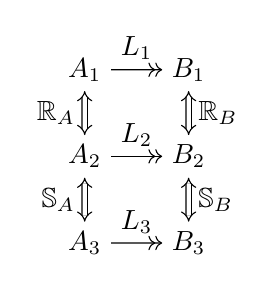
\begin{tikzpicture}[baseline=0.6mm,xscale=0.66,yscale=0.55]
    \node (A1) at (-1,  2) {$A_1$};
    \node (A2) at (-1,  0) {$A_2$};
    \node (A3) at (-1, -2) {$A_3$};
    \node (B1) at ( 1,  2) {$B_1$};
    \node (B2) at ( 1,  0) {$B_2$};
    \node (B3) at ( 1, -2) {$B_3$};
    \draw (A1) edge[->>] node[auto] {$L_1$} (B1);
    \draw (A2) edge[->>] node[auto] {$L_2$} (B2);
    \draw (A3) edge[->>] node[auto] {$L_3$} (B3);
    \begin{scope}[double equal sign distance, {Implies[]}-{Implies[]}]
      \draw (A1) edge[double] node[auto,swap] {$\mathbb{R}_A$} (A2);
      \draw (B1) edge[double] node[auto] {$\mathbb{R}_B$} (B2);
      \draw (A2) edge[double] node[auto,swap] {$\mathbb{S}_A$} (A3);
      \draw (B2) edge[double] node[auto] {$\mathbb{S}_B$} (B3);
    \end{scope}
  \end{tikzpicture}
  $
  \caption{Simulation identity and vertical composition}
  \label{fig:simcomp}
\end{figure}
%}}}

%}}}

%}}}
        % 3-4 pages
\section{Verified Compilation with a Nominal Memory Model}
\label{sec:nominal}

In this section, we describe the limitations of the block-based
memory model and present our new 
{\em nominal memory model} which removes the global constraints for
managing memory blocks and enables flexible memory structures for open
programs and concurrent threads.

\subsection{Problems with the Block-Based Memory Model}
\label{ssec:nominal-bbmm}

In the block-based memory model, the memory space is represented as a
countably infinite set of blocks where each block is given a unique
identifier called its \emph{block id} (denoted by $b$, represented
as postitive numbers). The entire memory space is
divided into two parts by a special block id called
\emph{\nextblock}. A block with id less than \nextblock has been
allocated (called a \emph{valid block}). Otherwise, it has not been
allocated yet (called an \emph{invalid block}). \nextblock---initially
with the value $1$---denotes the id of the next block to be allocated
and will be increased after each allocation. A valid memory block is a
finite array of bytes with a lower and upper bound. A \emph{memory
state} (denoted by $m$) consists of a mapping from addresses to
\emph{in-memory values} in valid blocks and the value of
\nextblock. Its type \coqe{mem} is defined in~\figref{sfig:memstate}
where \coqe{block} is the type of block ids, \coqe{Z} is the type of
integers, \coqe{memval} is the type of in-memory values, and
\coqe{$m$.(mem_contents) $b$ $o$ = $v$} iff $b$ is a valid block in
$m$ and $v$ is the in-memory value at the $o$-th memory cell (byte) of
$b$.

A pointer or a memory address is a pair $(b, o)$ where $b$ is the
memory block it points to and $o$ is an index to a memory cell in block
$b$ (also called an offset).
%
Pointer arithmetic is represented by adjustments to offsets. For
example, $(b, o) + n$ is defined as $(b, o+n)$.
%
This simple block-based abstraction already provides basic support for
memory isolation, in the sense that given a pointer to block $b_1$ we
can never reach $b_2$ by performing pointer arithmetic if $b_1 \neq b_2$.

\begin{figure}
  \begin{subfigure}[b]{.45\textwidth}
    \begin{coq}
Definition block : Type := positive.
Record mem: Type := { 
  mem_contents: block -> Z -> memval;
  nextblock: block; }.
    \end{coq}
    \caption{Blocks and Memory States}
    \label{sfig:memstate}
  \end{subfigure}
  \begin{subfigure}[b]{.5\textwidth}  
    \begin{coq}
alloc : mem -> Z -> Z -> mem \times block
free  : mem -> block -> Z -> Z -> $\some{\code{mem}}$
load  : mem -> chunk -> block -> Z -> $\some{\code{val}}$
store : mem -> chunk -> block -> Z -> val -> $\some{\code{mem}}$
    \end{coq}
    \caption{Memory Operations}
    \label{sfig:memops}
  \end{subfigure}
  \caption{Definitions for the Block-Based Memory Model}
  \label{fig:bbmem}
%  \vspace{-0.1cm}
\end{figure}

\figref{sfig:memops} shows the main operations over memory where
\coqe{val} is the type of \emph{regular values}:
%
\begin{coq}
   Inductive val := Vundef | Vint $i_{32}$ | Vlong $i_{64}$ | Vsingle $f_{32}$ | Vfloat $f_{64}$ | Vptr $(b,o)$.
\end{coq}
%
Here, \coqe{Vundef} represents undefined values, \coqe{Vptr $(b,o)$}
represents a pointer $(b,o)$, and the remaining forms denote 32- and
64-bit integer and floating point values.
%
\coqe{chunk} is the type of \emph{memory chunks} containing
information necessary for performing conversion between in-memory
values and regular values.
%
Note that the option type $\lfloor \rfloor$ is used to describe the
possible failure of some operations.  Given a memory state $m$, a
lower bound $l$ and a higher bound $h$, \coqe{alloc $m$ $l$ $h$}
returns a new block whose id is \coqe{$m$.(nextblock)} and whose valid
offsets are in the range of $[l,h)$. It also returns a new memory state
  where \nextblock is increased by $1$ and the newly allocated memory
  cells are initialized with undefined values.
%
Note that \coqe{alloc} \emph{always succeeds} because the memory space
has infinitely many blocks. The \coqe{free} operation frees memory
cells in a certain range. Given $m$, $k$ $b$ and $o$,
\coqe{load $m$ $k$ $b$ $o$}
loads a value starting from the address $(b,o)$ such
that the size and type of value are determined by $k$.  Conversely,
\coqe{store} stores a value into a certain location in memory.

A main task of compilers is to transform abstract data structures
(e.g., stacks) for describing the semantics of the high-level source
languages into concrete data structures for the low-level target
languages. These transformations often operate on certain part of
memory and have local effects.

CompCert introduces \emph{injections} to capture such changes. An
injection $j$ is a partial function of type
\coqe{block -> $\some{\code{block} \times \code{Z}}$}, such that $j(b) =
\some{(b',o)}$ iff a block $b$ is inserted into block $b'$ at offset
$o$ by the transformation. If $j(b) = \none$ (we use $\none$ to
represent the \coqe{None} constructor), then $b$ is removed from the
memory after the transformation.

When proving the correctness of these memory-transforming passes, one
would expect that we could exploit the locality of memory
transformations to construct intuitive proofs. For example, for
\code{SimplLocals}, \coqe{Cminorgen} and \coqe{Stacking}, one would
like to exploit the facts that \emph{1)} blocks for global definitions
are unchanged, and \emph{2)} the changes to individual stack frames
cannot interfere with each other. However, it is impossible to
formalize these facts directly because we can neither distinguish
blocks for global definitions from blocks in stack frames, nor tell
the differences between blocks in different stack frames: they are all
indexed by positive numbers. This problem is exactly caused by
\textbf{Inflexibility 1} introduced in~\S\ref{ssec:intro-nmm}.


Verification techniques for open programs are compositional only if
the semantics of open programs are compatible with each other.
However, the existence of a global \nextblock makes this compatibility
very difficult to establish, even when different open programs operate
on completely separate memory regions.
\ignore{
\begin{wrapfigure}[12]{r}{0.5\textwidth}
  \begin{tikzpicture}[scale=0.6, every node/.style={scale=0.9},auto]
    \def\bh{0.2cm}
    \tikzstyle{af}=[draw,minimum width=0.5cm, minimum height=0.5cm, rounded corners=.05cm];
    
    \node[af,fill=yellow] (t1f) {$f$};
    \node[af, below=\bh of t1f, fill=yellow] (t1g) {$g$};
    \node[af, below=\bh of t1g, pattern = north east lines] (t1i) {};
    \node[af, below=\bh of t1i, pattern = north east lines] (t1j) {};
    \node[af, below=\bh of t1j, fill=yellow] (t1h) {$h$};
    %% \node[draw = none, below left =\bh and -0.1cm of t1h, rotate = 90] (t1end) {$\ldots$};
    
    \draw[->,>=stealth] (t1f) -- (t1g);
    \draw[->,>=stealth] (t1g) -- (t1i);
    \draw[->,>=stealth] (t1i) -- (t1j);
    \draw[->,>=stealth] (t1j) -- (t1h);
    \draw[->,>=stealth] (t1h) -- ($(t1h.south) + (0cm, -0.3cm)$);

    \node[above = 0.1cm of t1f] {Thread $1$};

    \node[af, right = 2cm of t1f, pattern = north east lines] (t2f) {};
    \node[af, below=0.22cm of t2f, pattern=north east lines] (t2g) {};
    \node[af, below=\bh of t2g,fill=green] (t2i) {$i$};
    \node[af, below=\bh of t2i,fill=green] (t2j) {$j$};
    \node[af, below=\bh of t2j, pattern=north east lines] (t2h) {};
    %% \node[draw = none, below left =\bh and -0.1cm of t2h, rotate = 90] (t2end) {$\ldots$};

    \draw[->,>=stealth] (t2f) -- (t2g);
    \draw[->,>=stealth] (t2g) -- (t2i);
    \draw[->,>=stealth] (t2i) -- (t2j);
    \draw[->,>=stealth] (t2j) -- (t2h);
    \draw[->,>=stealth] (t2h) -- ($(t2h.south) + (0cm, -0.3cm)$);

    \node[above = 0.1cm of t2f] (t2txt) {Thread $2$};

    \node[draw=none, right = 1cm of t2i] (comp) {\large\bf $\Longrightarrow$};
    \node[draw=none, above = 0.1cm of comp] {\small \emph{Thread Linking}};

    \draw[->, dashed, >=stealth] (t1g) -- node [sloped, above] {\small \emph{yield}} (t2i);
    \draw[->, dashed, >=stealth] (t2j) -- node [sloped, above] {\small \emph{yield}} (t1j);


    \node[af, right = 3cm of t2f,fill=yellow] (tf) {$f$};
    \node[af, below=\bh of tf,fill=yellow] (tg) {$g$};
    \node[af, below=\bh of tg,fill=green] (ti) {$i$};
    \node[af, below=\bh of ti,fill=green] (tj) {$j$};
    \node[af, below=\bh of tj,fill=yellow] (th) {$h$};
    %% \node[draw = none, below left =\bh and -0.1cm of th, rotate = 90] (tend) {$\ldots$};

    \draw[->,>=stealth] (tf) -- (tg);
    \draw[->,>=stealth] (tg) -- (ti);
    \draw[->,>=stealth] (ti) -- (tj);
    \draw[->,>=stealth] (tj) -- (th);
    \draw[->,>=stealth] (th) -- ($(th.south) + (0cm, -\bh)$);
    
    \node[right = 2cm of t2txt] {Threads $\{1,2\}$};
    

  \end{tikzpicture}
  \vspace{-0.2cm}
  \caption{\scriptsize{}Linking of Multiple Stacks into a Single Stack in CCAL}
  \vspace{-0.2cm}
  \label{fig:stack-linking}
\end{wrapfigure}
}
We take the compilation and linking of Certified Concurrent
Abstraction Layers (CCAL) as an example to illustrate the above
problem~\cite{ccal18}.
\ignore{
A concurrent certified abstraction layer $L$
consists of shared and private memory states, abstract states, and a
set of possibly shared primitive operations (like external
functions). The semantics of a language (\eg, C or assembly) built on
top of $L$ forms an abstract machine in which concurrent programs can
be formally described.
}
%
A CCAL object is a formally verified open program built on top of some
layer $L$. A multi-threaded program is developed by abstracting
individual threads into CCAL objects. These objects are then
compiled by an extension of CompCert called Thread-Safe CompCertX into
assembly code. Finally, CCAL objects need to be linked together to
form a complete program. 

For the above linking to be possible, the views of memory of CCAL
objects must be compatible with each other. Achieving this
compatibility is non-trivial since 
a new stack block is
allocated for every function call in CompCert's assembly. To
link threads together, it is necessary for each thread to have
the same sequences of
stack blocks and \nextblock, meanwhile preventing one
thread from accessing the private stack memory of the others.
%
%
\ignore{
To solve the above problem, the authors of Thread-Safe
CompCertX~\cite{ccal18} modify the assembly semantics so that when a
thread yields to its context, a sequence of dummy stack blocks is
allocated to increase \nextblock in accordance with the actual
allocation of stack blocks by the context. Moreover, to avoid any
interference between memory operations on the stacks in different
threads, the dummy blocks do not carry any read or write
permission---they are ``dead'' memory cells from the perspective of
the focused thread. With those devices, it is possible to ``thread''
the private stack frames of each thread into a single stack. As an
example, the linking of stacks for two threads is depicted in
\figref{fig:stack-linking}. Here, the call to the yield primitive from
thread $1$ to $2$ in the function $g$ allocates two dummy blocks
(marked with diagonal lines) for the corresponding execution in thread
$2$. Accesses to these dummy blocks are invalid in thread $1$.


The solution above has two problems.
%
First, intuitively, each thread should have it own private stack:
the context should not interfere with operations on this stack.
Contrary to this assumption, the growth of dummy frames depends
on how contextual threads change \nextblock. This introduces
unnecessary complication to verification of compilation.
%
Second, in the linked program, stack frames for different threads are
interleaved with each other. This makes the semantics of
linked programs much more complex. It is also extremely difficult to
further verify their compilation to actual machine code where each
thread should have its own contiguous and private stack.
%
}
These problems are exactly caused by
\textbf{Inflexibilities 2 and 3} in~\S\ref{ssec:intro-nmm}.

\subsection{The Nominal Memory Model}
\label{ssec:nominal-nmm}

We solve the above problems by getting rid of the inflexibilites of
the block-based memory model through a generalization based on nominal
techniques.

Nominal techniques~\cite{pitts-nominal,gabby2002} provide a
mathematical foundation for managing named resources. 
%
In this setting, any countably infinite set $\nameset{A}$ can
represent a set of available names. Elements in these sets are called
\emph{atomic names} (or simply \emph{names} in short). Dependency of
objects upon names is captured by the notions of \emph{permutations}
and \emph{supports}. A permutation $\pi$ is a bijection from
$\nameset{A}$ to itself that only renames a finite subset of names in
$\nameset{A}$. Given a set of objects $X$ and some $x \in X$, $A
\subseteq \nameset{A}$ supports $x$ (or $A$ is a support of $x$) iff,
for any permutation $\pi$ on $\nameset{A}$ that is an identity mapping
for names in $A$, we have $\pi \cdot x = x$ where $\_ \cdot \_$
denotes the ``application'' (known as an \emph{action}) of $\pi$ to the
object $x$. This effectively means that $x$ is independent of any name
outside of $A$.
%
Only objects that can be supported by a finite set of names are of
interest to us.
%
A binary relation called \emph{freshness} makes the independence
relation concrete. A name $a\in \nameset{A}$ is fresh w.r.t. $x$
(written as $\freshness{a}{x}$) iff $x$ is supported by some finite set $A
\subseteq \nameset{A}$ and $a \not\in A$.

\begin{figure}[t]
\begin{coq}
  Module Type BLOCK.
    Parameter block : Type.
    Parameter eq_block : $\forall\app x\app y: \scode{block}, \sumbool{x=y}{x \neq y}$.
  End BLOCK.

  Module Type SUP.
    Parameter sup: Type.
    (** Operations *)
    Parameter sup_empty : sup.  (* Empty support *)
    Parameter fresh_block : sup -> block.  (* Generation of fresh blocks *)
    Parameter sup_incr : sup -> sup.  (* Increment of supports *)
    Parameter sup_in : block -> sup -> Prop.   (* Check validity of block ids *)
    (** Properties *)
    Parameter sup_dec : $\forall\app b\app s, \sumbool{\scode{sup\_in}\app b\app s}{\neg \scode{sup\_in}\app b\app s}$.
    Parameter empty_in: $\forall\app b, \neg \scode{sup\_in}\app b\app \scode{sup\_empty}$.
    Parameter freshness : $\forall\app s, \neg \scode{sup\_in}\app (\scode{fresh\_block}\app s)\app s$.
    Parameter sup_incr_in : $\forall\app a\app s, \scode{sup\_in}\app a\app (\scode{sup\_incr}\app s) 
    \leftrightarrow a = (\scode{fresh\_block}\app s) \lor \scode{sup\_in}\app a\app s$.
  End SUP.  
\end{coq}
  \vspace{-0.2cm}
  \caption{Interfaces of the Nominal Memory Model}
  \label{fig:nm-interface}
  \vspace{-0.1cm}
\end{figure}

The above concepts can be used to characterize the block-based
memory model. By taking memory states as objects containing names, 
we adopt the following analogies:
%
\begin{itemize}\itemsep 0pt
\item Block ids represent names that memory states depend upon;
\item Given a memory state $m$, the set of valid blocks in $m$
  represents a support of $m$;
\item Given a memory state $m$, its \nextblock is fresh w.r.t. $m$.
\end{itemize}
%
Note that the set of valid blocks is always finite. To some extent, the
existing memory operations in CompCert already exploit the properties
of atomic names and supports. For example,
\coqe{alloc} always succeeds because there is always an infinite amount
of ids outside the set of valid blocks.

However, the block-based memory also makes rigid assumptions
about names and supports:
%
\begin{itemize} \itemsep 0pt
\item Block ids are fixed to positive numbers;
\item For any memory state $m$ whose \nextblock is $n$, its support
  must be the fixed set of consecutive numbers $\{1,\ldots,n-1\}$;
\item For any memory state $m$ whose \nextblock is $n$, its fresh
  block must be assigned with the id $n$.
\end{itemize}
%

We remove these rigid assumptions and generalize the block-based
model into the nominal memory model by introducing an
abstraction of block ids and supports as module types, as shown
in~\figref{fig:nm-interface}.
%
By the definition of \coqe{BLOCK}, block ids are names with decidable equality.
%
By the definition of \coqe{SUP}, a support type must be accompanied by
four kinds
of operations: checking the membership of blocks in supports
(\coqe{sup_in}), creating an empty support (\coqe{sup_empty}),
generating fresh blocks (\coqe{fresh_block}) and increasing supports
with new blocks (\coqe{sup_incr}). Furthermore, those operations must
satisfy some well-formedness properties. 

\begin{figure}
\begin{coq}
  Module Block <: BLOCK.
    Definition block := positive.         Definition eq_block := peq.
  End Block.

  Module Sup <: SUP.
    Definition sup := list block.         Definition sup_in ($b$: block) ($s$: sup) : Prop := $b \in s$.
    Definition sup_empty : sup := [].     Definition fresh_block ($s$: sup) := (find_max_pos $s$) + 1.
    Definition sup_incr ($s$ :sup) := $(\scode{fresh\_block }s) \cons s$.   $\qquad$ ...
  End Sup.  
\end{coq}  
  \vspace{-0.2cm}
  \caption{Block-based Memory Model as an Instance}
  \vspace{-0.1cm}
  \label{fig:bm-instance}
\end{figure}

We also note that the above generalization does not exactly match with the
standard definitions in nominal techniques. For example, \coqe{BLOCK} does not
enforce that block ids are from a countably infinite set. Instead,
the \coqe{freshness} property guarantees that any block fresh w.r.t a
support $s$ must not be already in $s$. Together with the totality of
\coqe{fresh_block}, it implies the existence of an infinite number of
block ids.
%
We also define supports to be any type that has the interface of
\coqe{SUP}, instead of a finite set of block ids. This generalization
allows us to instantiate \coqe{sup} with complex data structures for
formalizing memory space in fine-grained styles. 

To make use of the above interfaces, we instantiate block ids and
supports as follows:
%
\begin{coq}
  Module Block <: BLOCK. ... End Block.           Module Sup <: SUP. ... End Sup.
\end{coq}
%
Then the original \coqe{block} type is instantiated with
\coqe{Block.block}. Moreover, the memory state carries a support instead of
\nextblock:
%
\begin{coq}
  Record mem: Type := { mem_contents: block -> Z -> memval;   support: Sup.sup;}.
\end{coq}
%
The memory operations are adapted accordingly. For example, checking
of valid blocks is done by using \coqe{sup_in} instead of comparing
with \nextblock:
%
\begin{coq}
  Definition valid_block ($m$:mem) ($b$:block) := $b$ < $m$.(nextblock).   (* Old *)
  Definition valid_block ($m$:mem) ($b$:block) := sup_in $b$ $m$.(support).  (* New *)
\end{coq}
%
For another example, \coqe{alloc} now invokes \coqe{fresh_block} to
allocate a new block instead of consulting \nextblock.
The properties of all memory operations can be easily reestablished
because they are already ignorant of particular instantiations of block ids
and supports. 

Finally, the block-based memory model becomes a special case of the
nominal memory model, as depicted in~\figref{fig:bm-instance} where
\coqe{find_max_pos} finds the maximal positive number in a list.

\vspace*{-2ex}
\paragraph*{Proposed Research.}
As a preliminary evidence for its effectiveness, we have recently
successfully applied the nominal memory model to the full compilation
chain of CompCert to get Nominal CompCert~\cite{wang2022}.  We updated
the semantics of every language of CompCert by replacing the old
memory operations with the new one. We then also updated the
simulation proofs. Because the generalization of block ids and
supports is mostly orthogonal to the simulation proofs in CompCert,
the changes are minimal.

\vspace*{-2ex}
\paragraph*{Task 2a: Nominal CompCert with structural memory space.}
A big part of our proposed effort is to develop various instantiations
of the nominal memory model where the whole {\em memory space} is
divided into memory regions with well-defined structures and clear
roles. One promising design~\cite{wang2022} separates global memory
(for global variables and functions) from stack memory; and then
organizes the stack into a tree structure that mirrors the ``call
activation'' tree.  Because most memory transformations do not change
the order of function calls and returns, the stack tree remains stable
under compilation; this allows us to recover the locality decompose a
transformation on the entire stack into local transformations on
individual stack frames, which could lead to much simpler and more
intuitive proofs for memory injection phases.

\vspace*{-2ex}
\paragraph*{Task 2b: Norminal CompCertO for open programs.}
Another key task is to integrate the norminal memory model into our
new compositional verified compilation framework in
\S\ref{sec:compcerto}.  Compositional compilation needs to not only
keep track of how memory is transformed by internal functions, but
also do that for external functions.  If the context is fixed, the
transformation on contextual memory should always be described as
\emph{an identity mapping} from source to target memory blocks,
regardless of how complicated the memory transformation is for
internal executions.  However, this seemingly simple task is extremely
difficult to complete in the original CompCert because it lacks the
ability to distinguish memory blocks allocated by internal functions
from those by external ones. With the nominal memory model and its
instances, contextual memory can be separated from internal memory and
be reasoned about via a well-defined interface, leading to simpler and
more elegant correctness proofs for compiling certain kinds of open
programs. We believe that these techniques together with others we
have built on top of the nominal memory model could be particularly
beneficial in the general context of compositional compiler
correctness.

\ignore{
In CompCert, the complexity of memory injections is largely confined
to the correctness proofs of individual passes: injections are
existentially quantified as part of the simulation relation and do not
appear in the correctness statement itself.  This is possible because
memory states are not part of the externally observable behavior of
programs. This assumption must be relaxed in compositional extensions
of CompCert which model interactions between compilation units.  In
work such as Compositional CompCert~\cite{compcompcert},
CompCertX~\cite{dscal15,wang2019}, CompCertM~\cite{compcertm},
CASCompCert~\cite{cascompcert} and CompCertO~\cite{koenig21}, memory
states appear as part of the interactions between components.  As a
consequence, the memory relations used by compilation passes become
part of their correctness statements.  This makes correctness theorems
and the vertical composition of passes much more complex.

Our techniques based on the nominal memory model have the potential to
significantly simplify the above proofs from the following
perspectives.  First, the evolving Kripke worlds used in compositional
compiler correctness are used to store both memory injections (which
can be determined ahead of time using more structural injection
functions) and additional permission information (which could be
stored in our model as part of the information associated with block
identifiers).  As a result, by incorporating our approach, it may be
possible to eliminate Kripke worlds entirely, which would
significantly simplify the semantic frameworks used in these projects.
Moreover, our techniques could help isolate private memory as internal
states, for example through the use of a partial commutative monoid
structure on memory states which would facilitate splitting and
merging private memory regions used by individual components.
Finally, they could provide a seamless way to incorporate stack
awareness to compositional compilers of this kind.
}

\vspace*{-2ex}
\paragraph*{Task 2c: Norminal CompCertO for open threads}
We will extend Nominal CompCertO to support
multi-threaded programs. The existing solutions invented ad hoc
mechanisms~\cite{ccal18} to cope with the global \nextblock which
prevent further compilation to a realistic machine model in which each
thread has its own contiguous and private stack. We plan to
instantiate supports with multiple stack trees where we can grow
the stacks individually without interference with each other, thereby
eliminating the problems with \nextblock.



          % 3-4 pages
\section{Compositional Verified Compilation into ELF Object Files}

Together with his students, PI Shao has recently developed
CompCertELF~\cite{compcertelf20}, the first extension to CompCert that
supports verified compilation from C programs all the way to a
standard binary file format, i.e., the ELF object format.  However,
CompCertELF only supports {\em{}verified separate
compilation}~\cite{sepcompcert} which cannot handle compositional linking of
heterogeneous components.  For this proposal, we will integrate the
technologies in CompCertELF into Nominal CompCertO to build an {\em
  end-to-end and compositional verified compiler} that can compile C
components all the way into ELF object files.

\vspace*{-2ex}
\paragraph*{Task 3a: Stack-Aware Nominal CompCertO.}
To support concrete memory layout required by the binary machine code,
we will first extend Nominal CompCertO to support compilation with a
single, continuous, and finite stack by incorporating the key ideas in
Stack-Aware CompCert~\cite{wang2019,compcertelf20}.  Stack-Aware
CompCert explicitly manages the call stack by adding a data type
called \emph{abstract stack} to memory states. The abstract stack
records the history of memory consumption incurred by stack allocation
and maintains fine-grained \emph{stack permissions}. By exploiting
that information, Stack-Aware CompCert achieves contextual compilation
of single-threaded C programs into an assembly language that is aware
of a single and finite stack.  In our structured nominal memory model,
the abstract stack can be readily absorbed into the support. We can
drop stack permissions from the abstract stack in Stack-Aware CompCert
because CompCertO already separately enforces them as part of its
reasoning framework (e.g., simulation conventions).  Furthermore, by
enriching supports with multiple abstract stacks following the idea of
Task 2d, we will build Multi-Stack Nominal CompCertO which can compile
multi-threaded programs onto multi-stack machine models. These ideas
will form a complete solution to thread-safe contextual compilation
needed to support CCAL~\cite{ccal18}.

\vspace*{-2ex}
\paragraph*{Task 3b: Verified compilation into relocatable ELF files}
CompCertELF is built on top of Stack-Aware CompCert. In essence, it
modifies and extends Stack-Aware CompCert's compilation chain with a
\emph{verified assembler} that transforms the realistic assembly
programs output by Stack-Aware CompCert to sequences of bytes that
represent relocatable ELF files.  This assembler consists of several
passes that successively merge code and data into atomic blocks (known
as sections), generate information for relocation and linking (such as
symbol tables and relocation tables), encode the assembly instructions
and the global data into their binary forms, and finally embed them
into the ELF format with meta-data (such as section headers and ELF
headers). A big part of this task is to leverage the rich structure
from the nominal memory model to enable richer ABIs.  Another
challenge is to develop automation support building certified
instruction encoders and decoders for different machine
architectures~\cite{xu21}.

\vspace*{-2ex}
\paragraph*{Task 3c: Certified compositional ELF linker and loader}
To support end-to-end certified linking, CompCertELF has to prove
compilation commutes with two different linkers: one used in CompCert
and the other for relocatable object files. On one hand, in CompCert,
the linker views programs as partial mappings from identifiers to
global definitions. Therefore, it is insensitive to and may
arbitrarily rearrange the order of definitions. On the other hand, to
generate relocatable object files, the function and variable
definitions are merged into atomic sections following some particular
order. The ELF linker simply concatenates sections of the same type
together like they are ``black boxes.''  Here, the order in which
definitions are merged and sections are concatenated significantly
affects the result of linking.  The consequence is that commutativity
between linking and compilation breaks at the transitional phase from
CompCert to the assembler where the latter links programs as
relocatable objects. We believe that the language interfaces in
CompCertO and the richer permutation support in our nominal memory
model can provide a better and cleaner solution toward a certified
linker and loader.

      % 1 page
%% For double-blind review submission, w/o CCS and ACM Reference (max submission space)
\documentclass[acmsmall,review,anonymous]{acmart}\settopmatter{printfolios=true,printccs=false,printacmref=false}
%% For double-blind review submission, w/ CCS and ACM Reference
%\documentclass[acmsmall,review,anonymous]{acmart}\settopmatter{printfolios=true}
%% For single-blind review submission, w/o CCS and ACM Reference (max submission space)
%\documentclass[acmsmall,review]{acmart}\settopmatter{printfolios=true,printccs=false,printacmref=false}
%% For single-blind review submission, w/ CCS and ACM Reference
%\documentclass[acmsmall,review]{acmart}\settopmatter{printfolios=true}
%% For final camera-ready submission, w/ required CCS and ACM Reference
%\documentclass[acmsmall]{acmart}\settopmatter{}


%% Journal information
%% Supplied to authors by publisher for camera-ready submission;
%% use defaults for review submission.
\acmJournal{PACMPL}
\acmVolume{1}
\acmNumber{CONF} % CONF = POPL or ICFP or OOPSLA
\acmArticle{1}
\acmYear{2018}
\acmMonth{1}
\acmDOI{} % \acmDOI{10.1145/nnnnnnn.nnnnnnn}
\startPage{1}

%% Copyright information
%% Supplied to authors (based on authors' rights management selection;
%% see authors.acm.org) by publisher for camera-ready submission;
%% use 'none' for review submission.
\setcopyright{none}
%\setcopyright{acmcopyright}
%\setcopyright{acmlicensed}
%\setcopyright{rightsretained}
%\copyrightyear{2018}           %% If different from \acmYear

%% Bibliography style
\bibliographystyle{ACM-Reference-Format}
%% Citation style
%% Note: author/year citations are required for papers published as an
%% issue of PACMPL.
\citestyle{acmauthoryear}   %% For author/year citations

% \documentclass[sigplan,10pt,authordraft]{acmart}
% \setcopyright{none}

% Packages {{{
%\usepackage{geometry}
%\usepackage[colorlinks]{hyperref}
\usepackage{ebproof}
%\usepackage{amsmath}
%\usepackage{amsthm}
%\usepackage{amssymb}
%\usepackage{libertine}
\usepackage{stmaryrd}
\usepackage{cmll}
\usepackage{tikz}
\usepackage{tikz-cd}
\usepackage{bbm}
\usetikzlibrary{calc}
\usepackage{minted}
\usepackage{subcaption}
\usepackage{graphicx}
\graphicspath{ {./images/} }
%}}}

% Commands {{{
% Some of the macros I defined trip up latexdiff,
% so I separate them in this file.
% vim: foldmethod=marker

% Notations
\newcommand{\kw}[1]{\ensuremath{ \mathsf{#1} }}
\newcommand{\ifr}[1]{\mathrel{[{#1}]}}
\newcommand{\que}{\circ}
\newcommand{\ans}{\bullet}
\newcommand{\vref}{\le_\kw{v}}
\newcommand{\mext}{\le_\kw{m}}
\newcommand{\refby}{\preceq}
\newcommand{\scref}{\sqsupseteq}
\newcommand{\screfd}{\sqsubseteq}
\newcommand{\unitset}{\mathds{1}}

% Multi-letter language interfaces
\newcommand{\li}[1]{\mathit{#1}}
% Calling conventions (language interface boundaries)
\newcommand{\cc}[2]{{ \kw{#1#2} }}

% Pointers for justified sequences %{{{

% Parameters
\newcommand{\pshift}{1.6ex}
\newcommand{\pcdist}{1}
\newcommand{\pcangle}{60}

% Pointer hook
\newcommand{\ph}[1]{%
  \tikz[remember picture]{\coordinate (#1);}}

% Pointer to
\newcommand{\ptc}[2]{%
  \tikz[remember picture,baseline,>={Latex[round,length=3.6pt]}]{
    \draw[->,#2]
      let \p{dest} = (#1),
          \n1 = {pow(veclen(\x{dest}, \y{dest}), 0.5) * 1.5},
          \p1 = ($(0,0)+(0,\pshift)$),
          \p4 = ($(\x{dest},0)+(0,\pshift)$),
          \p2 = ($(\p1)!\n1*\pcdist!-\pcangle:(\p4)$),
          \p3 = ($(\p4)!\n1*\pcdist!+\pcangle:(\p1)$) in
        (\p1) .. controls (\p2) and (\p3) .. node[pos=0.5] (top) {} (\p4);
    \pgfresetboundingbox
    \path[use as bounding box] (0,0 |- top);
}}
\newcommand{\pt}[1]{%
  \ptc{#1}{gray}}
\newcommand{\bpt}[1]{%
  \ptc{#1}{black,thick,>={Latex[round,length=4pt]}}}

% TikZ setup
\pgfdeclarelayer{tint}
\pgfdeclarelayer{nodes}
\pgfsetlayers{tint,background,main,nodes}
\selectcolormodel{cmyk}

% Parameters for diagrams
\newcommand{\stens}{0.6}

% The intensity of colors in figures and row highlighting respectively.
% These should be the same, otherwise they are just confusing to look at
% side by side, especially on a printout.
\newcommand{\filltint}{!35}
\newcommand{\tbltint}{\filltint}

% Colors used in the World transitions section
\newcommand{\colorA}{ACMDarkBlue}
\newcommand{\colorB}{ACMDarkBlue}
\newcommand{\internalA}[1]{\textcolor{\colorA}{#1}}
\newcommand{\internalB}[1]{\textcolor{\colorB}{#1}}

% Refinement tiles {{{

\newenvironment{tile}[1]{%
  \begin{tikzpicture}[baseline,yscale=0.36,xscale=0.5]
    \figsize
    \tikzset{to path={
      .. controls ($(\tikztostart)!\stens!(\tikztostart -| \tikztotarget)$)
              and ($(\tikztotarget)!\stens!(\tikztotarget -| \tikztostart)$) ..
      (\tikztotarget) \tikztonodes}}
    \tikzset{#1}
    % Coordinates for things on the left
    \coordinate (TL) at (-1,1);
    \coordinate (L) at (-1,0);
    \coordinate (BL) at (-1,-1);
    \coordinate (TLB) at (-0.3,1);
    \coordinate (BLB) at (-0.3,-1);
    % Coordinates for things on the right
    \coordinate (TR) at (1,1);
    \coordinate (R) at (1,0);
    \coordinate (BR) at (1,-1);
    \coordinate (TRB) at (0.3,1);
    \coordinate (BRB) at (0.3,-1);
    % Center node, for crossing
    \coordinate (T) at (0,+1.5);
    \node[circle,inner sep=2pt] (C) at (0,0) {};
    \coordinate (B) at (0,-1.5);
    % Computed coordinates
    \coordinate (TLC) at ($(T-|L)$);
    \coordinate (BLC) at ($(B-|L)$);
    \coordinate (TRC) at ($(T-|R)$);
    \coordinate (BRC) at ($(B-|R)$);
}{%
  \end{tikzpicture}
}
\newcommand{\simproof}[2]{%
  \begin{pgfonlayer}{nodes}
    \node[draw,rectangle,fill=white,rounded corners=2pt,minimum height=0.5cm,minimum width=0.8cm] at #1 {#2};
  \end{pgfonlayer}
}
\newcommand{\drawsc}{%
  \draw[thick,rounded corners=1mm]
}
\newcommand{\filltop}[1]{%
  \begin{pgfonlayer}{tint}
    \fill[#1] (TLC) rectangle (R);
  \end{pgfonlayer}
}
\newcommand{\fillbot}[1]{%
  \begin{pgfonlayer}{tint}
    \fill[#1] (L) rectangle (BRC);
  \end{pgfonlayer}
}
\newcommand{\fillboth}[1]}}



%\newtheorem{definition}{Definition}
%\newtheorem{theorem}[definition]{Theorem}
\newtheorem{remark}{Remark}

\newcommand{\bdot}{\cdot}
\newcommand{\ISpec}{\mathbf{ISpec}}
%}}}

% Hyphenation patterns {{{
\hyphenation{Comp-Cert}
\hyphenation{Comp-CertO}
%}}}

% Top matter {{{

\title{%
  Refinement Conventions:
  Composing Certified Compilers and Certified Abstraction Layers}

\author{Yu Zhang}
\orcid{0000-0002-0778-3517}
\affiliation{
  \institution{Yale University}
  \city{New Haven}
  \state{CT}
  \country{USA}}
\email{yu.zhang@yale.edu}

\author{J\'er\'emie Koenig}
\orcid{0000-0002-3168-5925}
\affiliation{
  \institution{Yale University}
  \city{New Haven}
  \state{CT}
  \country{USA}}
\email{jeremie.koenig@yale.edu}

\author{Zhong Shao}
\orcid{0000-0001-8184-7649}
\affiliation{
  \institution{Yale University}
  \city{New Haven}
  \state{CT}
  \country{USA}}
\email{zhong.shao@yale.edu}

%}}}

\begin{abstract} %{{{
Despite significant progress
in the development of certified software,
the lack of interoperability between
verification techniques is an obstacle
to the construction of
large-scale, heterogeneous certified systems.
%
Compositional semantics
can address this challenge
by providing a common mathematical foundation
across certified components,
as proposed in recent work on
refinement-based game semantics.

To make this work,
one key challenge is to give
a formal account of
the relationship between
component interactions
at different levels of abstraction.
%
A partial answer is provided by CompCertO,
a certified C compiler
which uses a notion of \emph{simulation convention}
to relate source- and target-level interactions
of translation units.
%This facilitates compositionality
%for the correctness proofs of compiler passes,
%organizing them into a type structure
%reminiscent of double categories.

This paper introduces \emph{refinement conventions}
as an analogous construction
for refinement-based game semantics.
%
Refinement conventions generalize both
the simulation conventions of CompCertO
and the abstraction relations used in
certified abstraction layers.
%and give a proper strategy model
%for the language semantics of CompCertO.
%Refinement conventions can also be used
%to connect the concrete C and assembly language interfaces
%used in CompCertO
%with the more abstract signatures
%used in the strategy specification model
%of certified abstraction layers.
%This allows us to produce
We deploy them to
establish a refinement between
the bounded queue layer example of \citet{rbgs-cal}
and a concrete C implementation,
whose correctness proof can be composed
with that of CompCertO.

%In practice,
%even compositional \emph{proof techniques}
%are usually formulated with respect to a
%non-compositional, operational semantics.

%We propose a general approach to
%specification, refinement and abstraction
%in the context of compositional semantics.
%As a case study,
%we apply this methodology to the certified compiler CompCert
%and its recent compositional extension CompCertO.
%This allows us to interface CompCertO with
%a particularly simple theory of certified abstraction layers.

%Recent work proposes to use game semantics for
%refinement-based verification
%of complex systems.
%However,
%mechanizing game semantics in a proof assistant presents many challenges.
%%in part due to the complexity of most game models,
%%and in part because the mathematics used in traditional descriptions of games
%%are ill-suited to a type-theoretic formalization.
%We show that the \emph{template games} of P.-A. Melli\`es,
%and a recently proposed \emph{algebraic} formulation of game semantics
%provide a viable approach.
%We mechanize a simple game model in the Coq proof assistant,
%enriched with a dually nondeterministic refinement ordering.
%The result allows us to extend existing verification frameworks
%in various directions.
%
%First,
%we use the model to provide a coarse-grained denotational semantics
%of CompCert program components,
%and use it to characterize and soundly implement
%the traditional C control operators \texttt{setjmp} and \texttt{longjmp}.
%We show that games makes it possible to
%model aspects of the execution environments of programs
%and demonstrate the verification of a system involving
%two separate processes communicating through a pipeline.
%
%Then,
%we develop a theory of certified abstraction layers
%within our new model.
%By decoupling certified abstraction layers
%from their low-level CompCert semantics,
%and by imposing a stronger typing discipline
%on layer interfaces and implementations,
%we address long-standing limitations on their compositionality.
%In particular,
%we verify a page allocator
%which can be used by an arbitrary number of
%independent clients.
\end{abstract}
%}}}

\begin{document}

\maketitle

\section{Introduction} %{{{

Guaranteeing the reliability of computer systems
is a long-standing challenge.
A modern computer system involves
layer upon layer of complex hardware and software components.
Each layer relies for its correct operation
on the layers below,
such that a defect in any one of them
could prevent the overall system from
working as expected.

Certified software is a promising approach
to this problem.
However,
current methodologies do not permit
the end-to-end certification of
large-scale, heterogeneous systems.

\subsection{Certified Software}

%A certified program comes with a formal specification,
%which describes with mathematical precision
%the expected behavior of program.
%In addition to the program itself,
%developers must then produce
%a formal proof of correctness,
%which can be easily and mechanically checked by a third party.

A \emph{certified} program is accompanied by
a mechanized proof of correctness,
which can easily be checked by a third party.
Under the most expansive approach,
the construction of a certified program
starts with a formal semantics 
for the language in use,
mechanized in a general-purpose proof assistant.
We must then formulate a mathematical specification
in terms of this model,
and prove a correctness property
showing that a particular program indeed meets the specification.

Formal methods research
has developed an impressive array of
tools and proof techniques
which can be used to carry out this task.
Researchers have constructed
certified versions of many key system components,
including
operating system kernels \cite{sel4,popl15},
compilers \cite{compcert},
and even hardware designs \cite{kami}.
Unfortunately,
building a system out of reliable components
is not enough to ensure
the reliability of the system as a whole.

\subsection{Compositionality}

Two components can interact in faulty ways
even when each one is reliable on its own terms.
For example,
the assumptions made by one component
may not match the guarantees provided by another---%
two perfectly functional logic gates which do not agree
on the voltages representing 0 and 1
will not interact in a predictable manner.
% XXX find another example
Beyond this,
we have to ensure that the components
interact harmoniously
to realize a particular high-level function---%
say, that compatible logic gates
connected in a certain way will indeed
implement a half-adder circuit.
Hence, when assembling certified programs
as components of a larger system,
we also need to assemble their proofs of correctness,
as components of a larger proof
which certifies the system end-to-end \cite{deepspec}.

%Building on these successes,
%there have been attempts to build larger certified systems
%out of these certified components,
%using their specifications as interfaces
%between their correctness proofs \cite{deepspec,etc}.

Combining the correctness proofs
of disparate certified components
is often difficult,
because they
tend to use different semantic models and proof techniques.
As a result,
while researchers have sometimes been able to interface
components on a case-by-case basis,
no general methodology has emerged
for composing independently certified components
into larger certified systems.

The large body of research on compositional semantics
provides important tools for developing such a methodology.
Recent work incorporates specifications and refinement
into game semantics \cite{rbgs-cal},
with the aim to provide a model rich enough
to describe and connect
a wide range of certified components.
However,
\emph{abstraction} presents an additional challenge
which this work has not yet addressed.

\subsection{Abstraction}

As we build complex systems out of simpler components,
the techniques we use to model and reason about those systems
often have little in common with
the ones used to model and reason about the underlying components.
For example,
the mathematics of logical circuits---%
used to engineer microprocessors---%
have little in common with
the semantics of these processors' assembly languages.
In turn, assembly languages work very differently from
the operating system abstractions and
high-level languages used to develop application software.
As a result,
building large-scale certified systems
which operate across many levels of abstraction
requires more than
modeling interactions across their components.
We must also describe explicitly
the relationship between
different \emph{views} of the system
%and of its components
at different levels of abstraction.

%From an engineering perspective,
%describing the relationship between
%high-level abstractions and the
%low-level implementation of
%cross-component interactions is very common:
%examples include
%voltages vs. binary levels,
%calling conventions for CPU architectures,
%network protocols, etc.

For programming languages,
traditional examples of this phenomenon include
\emph{data refinement} \cite{dataref}
or simulation relations.
However,
while these examples
are ubiquitous in the context of operational semantics,
they only connect different views of
a system's \emph{internal} state.
%
By contrast,
there is little precedent
for this kind of abstraction
when it comes to the \emph{interactions} of
components with their environments.

A limited exception to this rule
is provided by the certified compiler CompCertO \cite{compcerto},
which uses \emph{simulation conventions}
to relate the interaction of the source and target programs
and model the compiler's calling convention.

\subsection{Contributions}

This paper builds on the concept of simulation conventions
to provide a general account of abstraction
in game semantics:
\begin{itemize}
  \item We identify \emph{formal adjunctions} in
    refinement-enriched categories
    as an expression of the relationship
    between high-level and low-level views
    of a given interface.
  \item We introduce \emph{refinement conventions}
    as a convenient way to describe adjunctions
    in the context of refinement-based game semantics.
  \item We use these constructions to
    embed CompCertO's language semantics
    and correctness theorem into this
    compositional model.
  \item Finally, we demonstrate the usefulness
    of our approach by refining abstract descriptions of
    \emph{certified abstraction layers}
    into concrete C implementations.
    The layers can be composed with each other
    and with the correctness proof of CompCertO.
\end{itemize}
Our starting point is
the interaction specification model
of refinement-based game semantics
proposed by \citet{rbgs-cal}.
We have mechanized it in the Coq proof assistant
and used it to formalize our work.

Section \ref{sec:mainideas}
provides some background and
an overview of our framework.
In \S\ref{sec:compcerto}
we discuss the semantic model used in CompCertO
and its meaning in terms of interaction specifications.
Refinement conventions are introduced in \S\ref{sec:refconv},
and we show how they can be used to express
CompCertO's semantics preservation theorem.
In \S\ref{sec:cal},
we build on these results
to carry out the modular verification of
a simple program,
with respect to abstraction layer specifications
formulated in simple, high-level terms.

%In principle,
%the use of a general-purpose proof assistant
%makes it possible to interface disparate certified components.
%However in practice,
%the maths we use for this makes it difficult.
%
%\subsection{Compositional Verification}
%
%In order to scale,
%verification methods must be compositional:
%it must be possible to break down the problem of verifying a large program
%into subproblems of manageable size.
%Small program components such as individual statements
%can then be verified with reasonable effort, or even automatically.
%
%In principle,
%compositional semantics can help.
%In practice,
%people use compositional \emph{proof techniques},
%shown to be sound directly wrt. operational semantics:
%program logics,
%logical relations on syntax,
%certified abstraction layers.
%
%Yet for large-scale heterogeneous systems,
%compositional semantics is a must (b/c of generality ---
%compositional proof techniques only operate
%for a set language/framework).
%Hence time is ripe to reexamine how
%denotational semantics can fit within the practice of verification.
%
%CompCertO gets some of the way there
%but the model is designed to map onto
%existing techniques and proofs in CompCert.
%As a result,
%it doesn't have the nice mathematical properties
%which would enable
%generality and large-scale reasoning.
%
%\subsection{Compositional Semantics}
%
%[Denotational semantics mostly been considered
%as a theoretical endaevor whose goal is to
%better understand programming languages and PL features
%from a mathematical point of view:
%what things does a language express,
%how can its structures be characterized.
%Gold standard = full completeness.]
%
%Typical paper:
%show a full abstraction result for language X or
%a technique to support feature Y.
%This leaves out
%specifications, refinement, abstraction
%which are the bread and butter of
%large-scale system construction and verification.
%
%To deploy compositional semantics in the context of verification,
%we must shift somewhat from this emphasis:
%\begin{itemize}
%  \item The ability to represent specifications,
%    which may or may not be definable as programs,
%%    runs counter to insistence on definability,
%%    although it could still be useful to identify
%%    a subset of the domain which corresponds to
%%    actual programs.
%  \item The prominent role of \emph{abstraction} and \emph{refinement}
%    in the context of verification
%    means they have to be taken more seriously
%\end{itemize}
%
%Proposal: Idea of a hierarchy of models \cite{act21,lics20}.
%
%Refinement-based game semantics.


%}}}

\section{Main Ideas} \label{sec:mainideas} %{{{

\begin{table} % Notations {{{
  \begin{tabular}{ll}
    \hline
    \textbf{CompCertO} \\
    Languages interfaces & $\mathcal{X, Y}$ \\
    Open transition systems &
      $L_1, L_2 : \mathcal{X} \twoheadrightarrow \mathcal{Y}$ \\
    Simulation conventions &
      $\mathbb{R}, \mathbb{S} : \mathcal{X} \Leftrightarrow \mathcal{Y}$ \\
    Abstracting simulation &
      $L_1 \le_{\mathbb{R} \twoheadrightarrow \mathbb{S}} L_2$ \\
    \hline
    Memory state & $m$ \\
    Runtime value & $v$ \\
    Function identifier & $f$ \\
    \hline
    Compilation unit & $M, N, M_1, M_2$ \\
    OLTS semantics & $\kw{Clight}(M)$ \\
    Multi-module program & $\bar{M}$ or $\vec{M}$ ? \\
    Semantics of multi-module program &
      $\kw{Clight}(M_1, M_2, \ldots) :=
       \kw{Clight}(M_1) \oplus \kw{Clight}(M_2) \oplus \cdots$ \\
    \hline
    \textbf{Interaction specifications} \\
    Effect signatures &
      $E, F, G$ + implicitly promoted language interfaces \\
    Strategy & $\sigma : E \rightarrow F$ (but can vary) \\
    Refinement conventions & $\rho : E^\sharp \leftrightarrows E^\flat$ \\
    Abstracting refinement &
      $\sigma \sqsubseteq_{\rho \rightarrow \gamma} \tau$ \\
    Embedding of an OLTS &
      $\llbracket L \rrbracket : \mathcal{X} \rightarrow \mathcal{Y}$ \\
    Embedding of a simulation convention &
      $\llbracket \mathbb{R} \rrbracket : \mathcal{X} \leftrightarrows \mathcal{Y}$\\
    Queries, replies & $q \in E^\que$, $r \in E^\ans$, $\hat{q}, \check{q}$ \\
    % FIXME: what when we have E -> F and two kinds of queries/replies
    \hline
    \textbf{CertiKOS-style strategy layers} \\
    Layer interface & $L : 1 \rightarrow \mathcal{X}@D$ (or $K$, $U,V,W$) \\
    Layer implementation & $M \in \kw{Clight}$ (as before) \\
    Abstraction relations & $R \subseteq D^\sharp \times (D^\flat \times \kw{mem})$ \\
    Underlay vs. overlay & $L^\flat, L^\natural, L^\sharp$ \\
    Tensor product & $L_1 \otimes L_2$ \\
    Abrel $\rightarrow$ Refinement convention &
      $\hat{R} : \mathcal{C}@(D^\sharp \times \kw{mem}) \leftrightarrows
             \mathcal{C}@(D^\flat  \times \kw{mem})$ \\
    \hline
    \textbf{Abstract layers} \\
    Layer interface & $\Gamma : 1 \rightarrow E@D$ \\
    Layer implementation & $\Sigma : E \rightarrow F@D$ \\
    Abstraction relation & $\Lambda, \Theta \subseteq D^\sharp \times (D^\flat \times U)$ \\
    Abrel $\rightarrow$ Refinement convention &
      $\hat{\Theta} : D^\sharp \leftrightarrows
             (D^\flat  \times U)$ \\
    \hline
    \textbf{CertiKOS-Abstract Correspondence} \\
    Primitive correspondence & $\lambda : E \leftrightarrows \mathcal{X}$ \\
    getter-setter abstraction relation component &
      $\mu \subseteq U \times \kw{mem} $ \\
    Promoted to & $\hat{\mu} : \hat{U} \leftrightarrows \hat{\kw{mem}}$ \\
    \hline
  \end{tabular}
  \\
  \caption{Notations}
\end{table}
%}}}

This section gives a high-level overview
of our approach and of the relevant background.
We start with a general description of
refinement-based game semantics \cite{rbgs-cal}
and of the CompCertO certified compiler \cite{compcerto},
introduce our notion of refinement convention,
then explain how it can be used to interface
the interaction specification model
of certified abstraction layers
with concrete C programs
and with CompCertO's correctness theorem.

Throughout the paper,
we will use the simple C code presented in Figure~\ref{fig:code}
as a running example.
The code is typical in structure:
one translation unit
encapsulates a ring buffer data structure
behind a simple interface.
The second translation unit then uses the first
to implement a bounded queue.

Our ultimate goal is to use CompCertO's semantics
to verify each of these components in terms of
simple and abstract specifications.
We will then be able to compose these correctness properties
with each other and with CompCertO's semantics preservation theorem
to obtain a formal guarantee on the compiled and linked assembly code.

\begin{figure*} % fig:code {{{
  \centering
  \begin{subfigure}{0.45\textwidth}
\begin{minted}{C}
/* Encapsulated state */
static int c1, c2;
static V buf[N];

/* Accessors */
int inc1() { int i = c1++; c1 %= N; return i; }
int inc2() { int i = c2++; c2 %= N; return i; }
V get(int i) { return buf[i]; }
void set(int i, V val) { buf[i] = val; }
\end{minted}
  \subcaption{The translation unit $\kw{rb.c}$}
  \label{fig:rb}
  \end{subfigure}
  \hspace{4em}
  \begin{subfigure}{0.36\textwidth}
\begin{minted}{C}
/* Underlay signature */
extern int inc1(void);
extern int inc2(void);
extern V get(int i);
extern void set(int i, V val);

/* Layer implementation */
void enq(V val) { set(inc2(), val); }
V deq() { return get(inc1()); }
\end{minted}
  \subcaption{The translation unit $\kw{bq.c}$}
  \label{fig:bq}
  \end{subfigure}
  \caption{Our running example consists of two C components.
    The component $\kw{rb.c}$
    implements a ring buffer by encapsulating an array
    and two counters. The second component
    $\kw{bq.c}$ uses this interface to implement a
    bounded queue.}
  \label{fig:code}
%\caption{The state of a ring buffer,
%  made of two counters and a fixed-size array,
%  is encapsulated behind a simple interface.}
%\label{fig:rb}
%\caption{This component relies on the ring buffer primitives
%  provided in Fig.~\ref{fig:rb} to implement a bounded-size queue.}
%\label{fig:bq}
\end{figure*}
%}}}

\subsection{Semantics} %{{{

In order to subject a given system to mathematical analysis,
we must establish a mathematical model of its operation.
A~programming language semantics
does this in a systematic way
by assigning to each program $p \in P$
in a given language $P$
a description $\llbracket p \rrbracket \in D$
of its behavior within a domain $D$:
\[
    \llbracket {-} \rrbracket : P \rightarrow D
\]

There are many approaches
for constructing appropriate domains
and interpretation functions.
What distinguishes \emph{compositional} semantics
is that the interpretation function $\llbracket - \rrbracket$
can be defined alongside the syntactic structure of programs.
For example,
if two program phrases $p_1, p_2 \in P$
can be combined into $p_1 + p_2 \in P$,
the semantic domain will be equipped with an operation
$\oplus : D \times D \rightarrow D$
such that
\[
  \llbracket p_1 + p_2 \rrbracket =
  \llbracket p_1 \rrbracket \oplus
  \llbracket p_2 \rrbracket
  \,.
\]

When \emph{types} are involved,
the syntax and semantics
can be given in \emph{categorical} form.
The syntax is given as a category $\mathbf{P}$
where objects are types and typing contexts,
and where the morphisms $p : \Gamma \rightarrow A$
are program components which
are assigned type $A$ within a context $\Gamma$,
or more generally
which use resources in $\Gamma$ to provide an interface $A$.
The interpretation function
then becomes a functor
$\llbracket - \rrbracket : \mathbf{P} \rightarrow \mathbf{D}$
into a semantic category $\mathbf{D}$,
such that a program $p : \Gamma \rightarrow A \in \mathbf{P}$
is interpreted as
a morphism
$\llbracket p \rrbracket :
 \llbracket \Gamma \rrbracket \rightarrow
 \llbracket A \rrbracket
 \in \mathbf{D}$.

%}}}

\subsection{Specifications and Refinement} \label{sec:specs} %{{{

From the perspective of certified software engineering,
semantics allows us to formulate specifications and
correctness proofs
in the context of a well-behaved mathematical domain.
To make specifications and proofs compositional,
we can impose additional structure.

A desirable property of program behaviors
can be expressed as a predicate $\pi \in \mathcal{P}(D)$
over the semantic domain.
Moreover,
a set $\Pi \subseteq \mathcal{P}(D)$
of properties of interest
induces a \emph{refinement} ordering
${\sqsubseteq} \subseteq D \times D$.
A behavior $\sigma \in D$ is refined by $\tau \in D$
when %the following holds:
\[
  \sigma \sqsubseteq \tau \: :\Leftrightarrow \:
  \forall \pi \in \Pi \bdot
  \pi(\sigma) \Rightarrow \pi(\tau)
  \,.
\]
In fact, we can further interpret programs
into the domain $\mathcal{P}(\Pi)$,
associating to each one the set of properties
which it satisfies,
and using set inclusion as refinement.
%
Conversely,
if the domain is equipped \emph{a priori}
with a partial order $\sqsubseteq$,
its elements can themselves be regarded as properties:
\[
  \Pi \: := \:
    \{ \{ \tau \mid \sigma \sqsubseteq \tau \} \mid
       \sigma \in D \}
  \,.
\]

\paragraph{Stepwise Refinement}

When $D$ is rich enough,
specifications
can be given as elements of the domain;
the correctness of $p \in P$
with respect to a specification $\sigma \in D$
can then be expressed as
$
  \sigma \sqsubseteq \llbracket p \rrbracket
$.
Under this refinement-based approach,
specifications and correctness proofs
benefit from the compositionality of $\llbracket - \rrbracket$,
and correctness proofs can proceed by stepwise refinement.
For example,
when $\sigma_1 \sqsubseteq \llbracket p_1 \rrbracket$
and $\sigma_2 \sqsubseteq \llbracket p_2 \rrbracket$,
we can deduce:
\begin{equation} \label{eqn:speccomp}
  \sigma_1 \oplus \sigma_2 \:\sqsubseteq\:
  \llbracket p_1 \rrbracket \oplus
  \llbracket p_2 \rrbracket \:\sqsubseteq\:
  \llbracket p_1 + p_2 \rrbracket
  \,,
\end{equation}
as long as $\oplus$ is monotonic
with respect to refinement.

\paragraph{String Diagrams}

In a categorical setting,
these structure generalize to
order-enriched categories.
Every homset $\mathbf{D}(A, B)$
is equipped with a refinement ordering,
and the composition operation
\[
  {\circ}_{A,B,C} :
    \mathbf{D}(B, C) \times \mathbf{D}(A, B) \rightarrow
    \mathbf{D}(A, C)
\]
is a monotonic function.
Order-enriched categories can be seen as
\emph{thin} 2-categories,
where for $f, g : A \rightarrow B \in \mathbf{D}$
there is a 2-cell
$\alpha : f \Rightarrow g : A \rightarrow B$
if and only if $f \sqsubseteq g$.
Hence,
refinement proofs admit a
\emph{string diagram} calculus.

In a string diagram,
the objects of $\mathbf{D}$ are represented by regions of the plane.
A morphism $f : A \rightarrow B \in \mathbf{D}$
is represented by a vertical line
separating an $A$ region from a $B$ region,
with horizontal juxtaposition denoting composition.
A refinement property
$h \circ g \circ f \sqsubseteq v \circ u$
is represented as a point
connecting the lines $f$, $g$, $h$ above the point
to the lines $u$, $v$ below:
\[
  \begin{tile}{}
    \drawst (LT) node[above] {$f$} -- (TLI) -- (C);
    \drawst (T) node[above] {$g$} -- (TI) -- (C);
    \drawst (RT) node[above] {$h$} -- (TRI) -- (C);
    \drawst (C) -- (BLI) -- (LB) node[below] {$u$};
    \drawst (C) -- (BRI) -- (RB) node[below] {$v$};
    \node at (C) {$\bullet$};
  \end{tile}
\]
For example,
property (\ref{eqn:speccomp}) above
combines the properties
(a) $\sigma_1 \subseteq \llbracket p_1 \rrbracket$ and
(b) $\sigma_2 \subseteq \llbracket p_2 \rrbracket$ with
the compositionality property
(c) $\llbracket p_1 \rrbracket \circ \llbracket p_2 \rrbracket
     \sqsubseteq \llbracket p_1 + p_2 \rrbracket$
in the following way:
\[
  \text{[figure here]}
\]

String diagrams
provide a visual calculus for refinement proofs where
the associativity and monotonicity of composition
are made implicit.

%}}}

\subsection{Game Semantics} %{{{

A particular kind of compositional semantics
known as \emph{game semantics} uses
categories of games and strategies
as semantic domains.
The games used in this context are
two-player games
which model the interaction between
a program component (the proponent)
and its environment (the opponent).
The behavior of a component
is described as a proponent \emph{strategy}
in the game associated with the component's type.
The games do not usually involve
a winning condition. % or notion of payoff.

For heterogeneous certified systems,
this approach is interesting
because games provide a fairly general way to describe
the interfaces of certified components.
In the present work,
we use simple games
derived from signatures of the following kind.

\begin{definition}
An \emph{effect signature} is a set $E^\que$ of operations
together with a family of sets $\big( E^\ans_m \big)_{m \in E^\que}$
specifying an \emph{arity} for each operation.
We will write
\[
  E = \{ m : E^\ans_m \mid m \in E^\que \}
\]
\end{definition}

The game associated with $E$ simply consists of
a \emph{question} $m \in E^\que$ of the environment
followed by an \emph{answer} $n \in E^\ans_m$ of the system.
We will be more interested in the composite game $E \rightarrow F$,
which allows the \emph{system} to ask questions in $E$
before answering the environment's initial question in $F$.

At a high level of abstraction,
the interface provided by the program $\kw{rb.c}$ (\autoref{fig:rb})
and used by $\kw{bq.c}$ (\autoref{fig:bq})
can be described using the signature:
\[
  E_\kw{rb} := \{
    \kw{inc1} {:} \mathbb{N},
    \kw{inc2} {:} \mathbb{N},
    \kw{set}[i, v] {:} \mathbbm{1},
    \kw{get}[i] {:} V \mid
    i \in \mathbb{N}, v \in V \}
\]
Note that there are individual operations
$\kw{set}[i, v]$ and $\kw{get}[i]$
for every possible value of the arguments
$i \in \mathbb{N}$ and $v \in V$.
In such circumstances,
we will sometimes use the notation
\[
  E_\kw{rb} := \{
    \kw{inc1} : \mathbb{N}, \:
    \kw{inc2} : \mathbb{N}, \:
    \kw{set} : \mathbb{N} \times V \rightarrow \mathbbm{1}, \:
    \kw{get} : \mathbb{N} \rightarrow V \}
  \,.
\]
The interface provided by $\kw{bq.c}$
is described by the signature:
\[
  E_\kw{rb} := \{
    \kw{enq} : V \rightarrow \mathbbm{1},
    \kw{deq} : V \}
\]

\paragraph{Plays and Strategies}

Since $\kw{bq.c}$
uses the operations of $E_\kw{rb}$ to
provide those of $E_\kw{bq}$,
its behavior
can be described as a proponent strategy for the game
$E_\kw{rb} \rightarrow E_\kw{bq}$.
Given a particular value $\diamond \in V$,
a \emph{play} in this game may look like the sequence of moves:
\[
  \kw{enq}[\diamond] \cdot
  \underline{\kw{inc2}} \cdot
  7 \cdot
  \underline{\kw{set}}[7, \diamond] \cdot
  * \cdot
  \underline*
  \:,
\]
where we have underlined the moves of the proponent
and where $* \in \mathbbm{1}$ is the unit value.
Traditionally,
\emph{strategies} are then defined as
the set of plays a component can generate,
depending on the environment's behavior.
For example,
the strategy
$\sigma_\kw{bq} : E_\kw{rb} \rightarrow E_\kw{bq}$
associated with $\kw{bq.c}$ is
\begin{align*}
  \sigma_\kw{bq} =
  \{ 
   &\kw{deq} \cdot
    \underline{\kw{inc1}} \cdot
    i \cdot
    \underline{\kw{get}[i]} \cdot
    v \cdot
    \underline{v} \,, \\
   &\kw{enq}[v] \cdot
    \underline{\kw{inc2}} \cdot
    i \cdot
    \underline{\kw{set}[i, v]} \cdot
    * \cdot
    \underline*
  \mid
    v \in V, i \in I
  \}
  \,.
\end{align*}
Here again,
set inclusion $\subseteq$
can serve as refinement.

\paragraph{Composition}

Suppose the strategy
$\sigma_\kw{rot} : E_\kw{bq} \rightarrow E_\kw{rot}$
implements %the signature
$E_\kw{rot} = \{ \kw{rot} : V \}$
with the following behavior:
\[
  \sigma_\kw{rot} := \{
    \kw{rot} \cdot
    \underline{\kw{deq}} \cdot
    v \cdot
    \underline{\kw{enq}[v]} \cdot
    * \cdot
    \underline{v}
    \mid v \in V
  \}
\]
That is,
an incoming call to $\kw{rot}$
uses the interface $E_\kw{bq}$
to first dequeue a value $v$,
push it back at the end of the queue,
then returns $v$.

The composite strategy
$\sigma_\kw{rot} \circ \sigma_\kw{bq} :
 E_\kw{rb} \rightarrow E_\kw{rot}$
lets the two components interact,
by replacing the calls
$\underline{\kw{deq}} \cdot v$
and
$\underline{\kw{enq}[v]} \cdot *$
in the plays of $\sigma_\kw{rot}$
by corresponding plays of $\sigma_\kw{bq}$.
The internal interactions between the two components
are then hidden to obtain the strategy:
\begin{align*}
  \sigma_\kw{rot} &\circ \sigma_\kw{bq} = \\
  \{
   &\kw{rot} \cdot
    \underline{\kw{inc1}} \cdot i \cdot
    \underline{\kw{get}[i]} \cdot v \cdot
    \underline{\kw{inc2}} \cdot j \cdot
    \underline{\kw{set}[j,v]} \cdot * \cdot
    \underline{v}
  \mid {} \\
   &i \in \mathbb{N}, \:
    j \in \mathbb{N}, \:
    v \in V
  \}
\end{align*}

\paragraph{Strategies as Specifications}

We have discussed in \S\ref{sec:specs}
the relationship between
properties, refinements and specifications.
One way to look at the construction of strategies
in game semantics
is to read plays as elementary properties
of the system being modeled.

Within a strategy,
a play essentially states:
``if the environment behaves in this way,
then the system should respond in that way''.
Program components are then characterized by
the set of such properties which they satisfy.
Under-constrained strategies can be refined by
more defined ones.
Over-constrained strategies---%
which contain plays
making incompatible demands of the system---%
cannot be implemented by concrete programs.

The union of $\sigma_1$ and $\sigma_2$
can only be refined by strategies which refine both:
\[
  \sigma_1 \cup \sigma_2 \subseteq \tau
  \quad\Leftrightarrow\quad
  \sigma_1 \subseteq \tau \:\wedge\:
  \sigma_2 \subseteq \tau
  \,.
\]
In other words,
unions correspond to \emph{angelic nondeterminism},
where the environment is free to rely on either behavior
because the system must exhibit both.
However,
to establish a complete refinement calculus
we also need a form of \emph{demonic} nondeterminism,
allowing us to formulate specifications such as
``the system may either return 0 or 1''.
Note that the set $\{0, 1\}$ is not appropriate in this case,
since it would simultaneously require the system
to return both 0 and 1.

%}}}

\subsection{Completely Distributive Lattices} %{{{

Semi-lattices provide the algebraic foundation
of traditional angelic \emph{or} demonic nondeterminism.
Completely distributive lattices
provide a similar foundation for
\emph{dual} nondeterminism,
which combines arbitrary angelic and demonic choices.

\begin{definition}
A \emph{complete lattice}
is a partially ordered set $\langle L, {\sqsubseteq} \rangle$
with all joins and meets.
This means in particular that $L$
has a least element $\bot = \bigsqcup \varnothing = \bigsqcap L$
and a greatest element $\top = \bigsqcap \varnothing = \bigsqcup L$.

A \emph{completely distributive} lattice
is a complete lattice which satisfies
the (equivalent) distributivity properties:
\begin{gather} \label{eqn:compdist}
  \bigsqcup_{i \in I} \bigsqcap_{j \in J_i} x_{ij} =
  \bigsqcap_{f \in \prod_i J_i} \bigsqcup_{i \in I} x_{i,f_i}
  \\
  \bigsqcap_{i \in I} \bigsqcup_{j \in J_i} x_{ij} =
  \bigsqcup_{f \in \prod_i J_i} \bigsqcap_{i \in I} x_{i,f_i}
\end{gather}
\end{definition}

These properties admit an intuitive game-theoretic interpretation.
Suppose the elements of $L$
are \emph{payoffs} in a zero-sum, two-player games
where the proponent and opponent
take turns making moves.
The proponent seeks to minimize the payoff.
If they can choose among the payoffs $(x_i)_{i \in I}$,
the outcome will be $\bigsqcap_i x_i$.
Conversely,
if the opponent can choose among $(y_j)_{j \in J}$,
the outcome will be $\bigsqcup_j y_j$.
Hence the expression
$\bigsqcap_i \bigsqcup_j x_{ij}$
denotes the result of a game where
the proponent first makes a choice $i \in I$,
the opponent then chooses $j \in J_i$,
producing the outcome $x_{ij}$.

We can reverse the order of these moves
by having the opponent play first
and pre-choose a strategy $f \in \prod_i J_i$.
The proponent then selects $i \in I$,
leading to the outcome is $x_{i,f_i}$.
At first glance,
this game is very different:
the proponent has access to much more information
and can make a decision based on the opponent's choice of strategy.
However,
the expressions $\bigsqcap_i \bigsqcup_j x_{ij}$
and $\bigsqcup_f \bigsqcap_i x_{i,f_i}$
are only concerned with the case where both players adopt
an optimal strategy.
In this particular scenario,
the opponent choices were in effect already known,
hence the proponent gains no advantage.

\paragraph{Free Completely Distributive Lattices}

Given a partially ordered set of elementary properties,
a rich specification model can be constructed as
the \emph{free completely distributive lattice}
generated by those properties \cite{augtyp,dndf}.
This construction can be characterized as follows.

\begin{definition}[Free completely distributive lattice]
The forgetful functor
$U : \mathbf{CDLat} \rightarrow \mathbf{Pos}$
from the category of completely distributive lattices
and complete homomorphisms
to the category of partially ordered sets
and monotonic functions
has a left adjoint
$\kw{FCD} : \mathbf{Pos} \rightarrow \mathbf{CDLat}$.
For a poset $A \in \mathbf{Pos}$,
we call $\kw{FCD}(A)$ the \emph{free completely distributive lattice}
generated by $A$.
\end{definition}

An explicit construction is given by \citet{augtyp}.
For our purposes,
the elements of $\kw{FCD}(A)$
will be terms of the form
\[
  \bigsqcup_{i \in I} \bigsqcap_{j \in J_i} \phi(a_{ij})
\]
identified up to the properties of completely distributive lattices.
The function $\phi : A \rightarrow \kw{FCD}(A)$
embeds the underlying partially ordered set
into $\kw{FCD}(A)$.

%}}}

\subsection{Interaction Specifications} %{{{

Refinement-based game semantics \cite{rbgs-cal}
combines these ideas to introduce a notion of
\emph{strategy specification},
which incorporates dual nondeterminism
into the strategies of game semantics.

In the \emph{interaction specification} model,
strategies are constructed in terms of a monad $\mathcal{I}_E(X)$.
This monad describes computations
which may perform calls as described by the signature $E$,
and eventually produce a result in the set $X$.
To define $\mathcal{I}_E(X)$,
we can start with a notion of plays of the form:
\[
  s \in P_E(X) ::=
    \underline{m} \mid
    \underline{m}ns \mid
    \underline{x}
  \qquad
  (m \in E^\que, n \in E^\ans_m, x \in X)
\]
The plays are ordered by the prefix relation.
Hence $\underline{m}$ describes a computation
which starts with a call $m$,
without placing any constraint on its subsequent behavior.
Interaction specifications are then obtained
using the free completely distributive lattice construction:
\[
  \mathcal{I}_E(X) := \kw{FCD}(P_E(X)) \,.
\]

In turn,
the interaction specification monad can be used to define
a category of effect signatures and strategy specifications.
A morphism $\sigma : E \rightarrow F$
gives for each possible question $m \in F^\que$
an interaction specification of type $\mathcal{I}_E(F^\ans_m)$:
\[
  \sigma^m \in \mathcal{I}_E(F^\ans_m)
  \qquad
  (m \in F^\que)
\]
The strategy $\sigma : E \rightarrow F$
can then be invoked by a computation $x \in \mathcal{I}_F(X)$,
so that we obtain the computation:
\[
  x[\sigma] \in \mathcal{I}_E(X) \,,
\]
where external interaction have been
replace by the behavior prescribed in
the strategy $\sigma$.
The composition of strategies can be defined
in terms of this operator,
so that for $\tau : F \rightarrow G$,
we obtain:
\[
  (\tau \circ \sigma)^m := \tau^m[\sigma]
  \qquad
  (m \in G^\que)
\]
We will call $\ISpec$ the resulting category
of effect signatures and strategy specifications.

%}}}

\subsection{CompCertO} \label{sec:mainideas:compcerto} %{{{

The certified C compiler CompCert \cite{compcert} is
written and verified in the Coq proof assistant.
CompCert comes with a semantics preservation theorem
which asserts that
the behavior of the compiled program
refines that of the source program.
This ensures that CompCert does not introduce any bugs
during compilation.
Moreover,
when code is verified at the source level,
the correctness proof of the code
can be combined with what of the compiler
to obtain formal guarantees
about the behavior of the compiled assembly program.
The CertiKOS operating system kernel
is one large project
which has made use of this capability \cite{popl15}.

\paragraph{Separate Compilation} %{{{

For applications of this kind,
the Clight language---%
a simplified dialect of C---%
is often used as the source language of CompCert.
The correctness theorem is then stated as
a \emph{separate compilation} \cite{sepcompcert} property:
\begin{equation} \label{eqn:scc}
  \begin{prooftree}
    \hypo{\forall i \cdot \kw{CompCert}(M_i) = M_i'}
    \infer1{\kw{Clight}[M_1 + \cdots + M_n]
      \le \kw{Asm}[M_1' + \cdots + M_n']}
  \end{prooftree}
\end{equation}
Here,
the translation units $M_1, \ldots, M_n$
are compiled to the assembly programs $M_1', \ldots, M_n'$.
The semantics of a source program $p$
is given as a labeled transition system $\kw{Clight}[p]$,
whereas the semantics of a target program $p'$
is given as $\kw{Asm}[p']$.
The linking operator $+$
combines translation units into a whole program,
and the relation $\le$ denotes a simulation property
between the resulting transition systems.

%}}}

\paragraph{Compositional Semantics} %{{{

Property (\ref{eqn:scc})
describes a situation where
multiple source files are compiled independently.
However,
the semantics itself
only describes the behavior of the linked whole program.
CompCertO modifies the semantic model used in CompCert
to describe the behavior of individual components
and model their interaction with the environment.
The compiler correctness property
is formulated in terms of this compositional semantics.
A first approximation of this property is:
\begin{equation} \label{eqn:ccc}
  \begin{prooftree}
    \hypo{\kw{CompCert}(M) = M'}
    \infer1{\kw{Clight}(M) \le \kw{Asm}(M')}
  \end{prooftree}
\end{equation}
Linking is modeled by a semantic operation $\oplus$
monotone with respect to simulations,
which satisfies
\[
  \kw{Asm}(M_1) \oplus \kw{Asm}(M_2) \le
  \kw{Asm}(M_1 + M_2)
  \,.
\]
Together,
these properties make it possible to formulate
a separate compilation theorem
similar to (\ref{eqn:scc}).
However,
\citet{compcerto} argues that
the compositional semantics of CompCertO
provides a more precise account 
of the guarantees offered by the compiler,
and a more flexible basis
for modeling heterogeneous systems.

%}}}

\paragraph{Key Challenge} %{{{

In the original closed semantics of CompCert,
the behavior of the source and target programs
can be compared directly:
there is no abstraction gap between the traces
of the source and target programs,
in the sense that
two corresponding traces will be equal.

The situation becomes more subtle in CompCertO.
The compositional semantics of CompCertO
reveals interactions between program components
which were previously hidden in the internal states
of the closed semantics.
However,
these interactions take very different forms
in the source program
(where they correspond to C function calls)
and in the target program
(where they correspond to assembly language jumps
in a particular register state).

%}}}

\paragraph{Language Interfaces} %{{{

To deal with the different forms
interactions take
across different languages,
CompCertO introduces a rudimentary form of typing
for its transition systems.
The interactions between a component and its environment
are described by \emph{language interfaces},
which are signatures of the form
$\{ m : E^\ans \mid m \in E^\que \}$,
where all operations share the same arity set $E^\ans$.

For example, C-~and assembly-level interactions
can be described as:
\begin{align*}
  \mathcal{C} &:=
    \big\{ f(\vec{v}) : \kw{val} \mathrel{\big|}
       f \in \kw{ident}, \vec{v} \in \kw{val}^* \big\}
  \\
  \mathcal{A} &:=
    \big\{ \mathit{rs} : \kw{val}^R \mathrel{\big|}
       \mathit{rs} \in \kw{val}^R \big\}
  \,,
\end{align*}
Here $f \in \kw{ident}$ is the identifier of
a C function to be called,
and $v \in \kw{val}^*$ specifies its actual arguments,
given a sequence of CompCert runtime values of type $\kw{val}$.
The arity simply corresponds to
the possible runtime values which the function may return.
At the assembly level,
both calls and returns communicate
the register state $\mathit{rs} \in \kw{val}^R$.
Register states assign runtime values
to the register names in the fixed set $R$,
which includes the program counter and stack pointer.

In addition,
all interactions in CompCertO
are annotated with a global memory state of type $\kw{mem}$,
a situation which we can describe using the construction:
\[
  E@\kw{mem} := \{ m@\mathit{ms} : N \times \kw{mem} \mid
                   (m : N) \in E, \mathit{ms} \in \kw{mem} \}
\]

Transition systems
are then assigned a type
$E \twoheadrightarrow F$,
where $E$ and $F$ are
language interfaces (usually the same one).
The types of Clight and assembly semantics
can be given as:
\begin{align*}
  \kw{Clight}(-) :
    \mathcal{C}@\kw{mem}
   &\twoheadrightarrow
    \mathcal{C}@\kw{mem}
  \\
  \kw{Asm}(-) :
    \mathcal{A}@\kw{mem}
   &\twoheadrightarrow
    \mathcal{A}@\kw{mem}
\end{align*}
A transition system of type $E \twoheadrightarrow F$
accepts incoming calls in $F$
and may perform outgoing calls in $E$.
In other words,
it describes a strategy of type $E \rightarrow F$
(see \S\ref{sec:compcerto} for details).

%}}}

\paragraph{Simulation Conventions} %{{{

It remains to specify the correspondence
between source- and target-level interactions.
To this end,
CompCertO introduces a notion of \emph{simulation convention}
between language interfaces.
A simulation convention $\mathbb{R} : E \Leftrightarrow F$
relates
the high-level questions in $E^\que$ and
the low-level questions in $F^\que$,
as well corresponding
high-level answers in $E^\ans$ and
low-level answers in $F^\ans$.
For example,
the simulation convention
$\mathbb{C} : \mathcal{C} \Leftrightarrow \mathcal{A}$
is used to formalize the compiler's
overall calling convention.

Simulations then operate with respect to
two different simulation conventions:
one for outgoing calls and one for incoming calls.
We will write
\[
  L_1 \le_{\mathbb{R}_E \twoheadrightarrow \mathbb{R}_F} L_2
\]
when the transition system
$L_1 : E_1 \twoheadrightarrow F_1$
is simulated by
$L_2 : E_2 \twoheadrightarrow F_2$
up to the outgoing convention
$\mathbb{R}_E : E_1 \Leftrightarrow E_2$
and the incoming convention
$\mathbb{R}_F : F_1 \Leftrightarrow F_2$.

\begin{figure} % fig:simcomp {{{
  $\begin{array}{c}
    \kw{id} : E \Leftrightarrow E
    \qquad
    L \le_{\kw{id} \twoheadrightarrow \kw{id}} L
    \\[1.5em]
   {\begin{prooftree}
    \hypo{\mathbb{R} : E_1 \Leftrightarrow E_2}
    \hypo{\mathbb{S} : E_2 \Leftrightarrow E_3}
    \infer2{\mathbb{R} \cdot \mathbb{S} : E_1 \Leftrightarrow E_3}
    \end{prooftree}}
    \\[1.5em]
   {\begin{prooftree}
    \hypo{L_1 \le_{\mathbb{R}_E \twoheadrightarrow \mathbb{R}_F} L_2}
    \hypo{L_2 \le_{\mathbb{S}_E \twoheadrightarrow \mathbb{S}_F} L_3}
    \infer2{
      L_1 \le_{\mathbb{R}_E \cdot \mathbb{S}_E \twoheadrightarrow
               \mathbb{R}_F \cdot \mathbb{S}_F} L_3}
    \end{prooftree}}
  \end{array}
  \:\:
  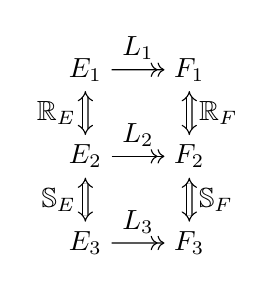
\begin{tikzpicture}[baseline=0.6mm,xscale=0.66,yscale=0.55]
    \node (A1) at (-1,  2) {$E_1$};
    \node (A2) at (-1,  0) {$E_2$};
    \node (A3) at (-1, -2) {$E_3$};
    \node (B1) at ( 1,  2) {$F_1$};
    \node (B2) at ( 1,  0) {$F_2$};
    \node (B3) at ( 1, -2) {$F_3$};
    \draw (A1) edge[->>] node[auto] {$L_1$} (B1);
    \draw (A2) edge[->>] node[auto] {$L_2$} (B2);
    \draw (A3) edge[->>] node[auto] {$L_3$} (B3);
    \begin{scope}[double equal sign distance, {Implies[]}-{Implies[]}]
      \draw (A1) edge[double] node[auto,swap] {$\mathbb{R}_E$} (A2);
      \draw (B1) edge[double] node[auto] {$\mathbb{R}_F$} (B2);
      \draw (A2) edge[double] node[auto,swap] {$\mathbb{S}_E$} (A3);
      \draw (B2) edge[double] node[auto] {$\mathbb{S}_F$} (B3);
    \end{scope}
  \end{tikzpicture}
  $
  \caption{Simulation identity and vertical composition}
  \label{fig:simcomp}
\end{figure}
%}}}

Simulations and simulation conventions
compose in the way depicted in \autoref{fig:simcomp}.
The two-dimensional types of simulations
are organized in a way reminiscent of double categories.
As such,
simulation proofs admit a string diagram calculus \cite{dcsd}
which extends the one presented earlier
with simulation conventions,
shown as horizontal lines.
In this framework,
the semantics preservation theorem of CompCertO
can be presented as:
\[
  \begin{prooftree}
    \hypo{\kw{CompCert}(M) = M'}
    \infer1{
      \kw{Clight}(M)
      \le_{\mathbb{C} \twoheadrightarrow \mathbb{C}}
      \kw{Asm}(M')}
  \end{prooftree}
  \qquad
  \mbox{[diagram]}
\]

In \autoref{sec:refconv},
we extend $\ISpec$ to a double category
using our generalized notion of \emph{refinement convention}.
This double category can embed
the transition systems,
simulation conventions, and
simulation properties of CompCertO.

%}}}

%}}}

\begin{figure*} % fig:cal {{{
  \begin{minipage}{.9\textwidth}
    \begin{align*}
      %
      % Overlay
      %
      & \fbox{$L_\kw{bq}$} &
        S_\kw{bq} &:= V^* \\
      \kw{enq} &: V \rightarrow \mathbbm{1} &
        L_\kw{bq}.\kw{enq}(v)@\vec{q} &:= \{ * @ \vec{q} v \mid |\vec{q}| < N \} \\
      \kw{deq} &: \mathbbm{1} \rightarrow V &
        L_\kw{bq}.\kw{deq}(*)@\vec{q} &:= \{ v @ \vec{p} \: \mid \vec{q} = v \vec{p} \}
      \\[1em]
      %
      % Implementation
      %
      & \fbox{$M_\kw{bq}$} &
        R &\subseteq S_\kw{bq} \times S_\kw{rb} \\
      M_\kw{bq}.\kw{enq}(v) &:= i \leftarrow \kw{inc}_2 ; \: \kw{set}(i, v) &
        \vec{q} \mathrel{R} (f, c_1, c_2) &\Leftrightarrow
        \: (c_1 \le c_2 < N \wedge
            \vec{q} = f_{c_1} \cdots f_{c_2-1}) \vee {}
      \\
      M_\kw{bq}.\kw{deq}(*) &:= i \leftarrow \kw{inc}_1 ; \: \kw{get}(i) &
        & \qquad \! (c_2 \le c_1 < N \wedge
            \vec{q} = f_{c_1} \cdots f_{N-1} f_0 \cdots f_{c_2 - 1})
      \\[1em]
      %
      % Underlay
      %
      & \fbox{$L_\kw{rb}$} &
        S_\kw{rb} &:= V^N \times \mathbb{N} \times \mathbb{N}
      \\
      \kw{set} &: \mathbb{N} \times V \rightarrow \mathbbm{1} &
        L_\kw{rb}.\kw{set}(i, v)@(f, c_1, c_2) &:=
        \{ *@(f', c_1, c_2) \mid i < N \wedge f' = f[i := v] \}
      \\
      \kw{get} &: \mathbb{N} \rightarrow V &
        L_\kw{rb}.\kw{get}(i)@(f, c_1, c_2) &:=
        \{ f_i@(f, c_1, c_2) \mid i < N \}
      \\
      \kw{inc}_1 &: \mathbbm{1} \rightarrow \mathbb{N} &
        L_\kw{rb}.\kw{inc}_1@(f, c_1, c_2) &:=
        \{ c_1@(f, c_1', c_2) \mid
           c_1' = (c_1 + 1) \mathop{\mathrm{mod}} N \}
      \\
      \kw{inc}_2 &: \mathbbm{1} \rightarrow \mathbb{N} &
        L_\kw{rb}.\kw{inc}_2@(f, c_1, c_2) &:=
        \{ c_2@(f, c_1, c_2') \mid
           c_2' = (c_2 + 1) \mathop{\mathrm{mod}} N \}
    \end{align*}
  \end{minipage}
  \caption{
    A certified abstraction layer
    $L_\kw{rb} \vdash_R M_\kw{bq} : L_\kw{bq}$
    implementing a bounded queue of size $N$
    using a ring buffer.
    The left-hand side of the figure shows
    the signatures of the overlay and underlay interfaces,
    and the code associated with the layer.
    The right-hand side shows primitive specifications
    and the simulation relation used by the correctness proof.
    Reproduced from \citet{rbgs-cal}.}
  \label{fig:cal}
\end{figure*}
%}}}

\subsection{Certified Abstraction Layers}\label{sec:mainideas:cal}

To an extent,
the formal tools required for the formulation of refinement conventions
are already present in the strategy specification model
of certified abstraction layers \cite[\S 3.7]{rbgs-cal}.
%
In this model,
the layer correctness property
\begin{equation} \label{eqn:layer}
  L_1 \vdash_R M : L_2
\end{equation}
asserts that the strategy specification
$M : E_1 \rightarrow E_2$
faithfully implements the \emph{overlay} interface
$L_2 : \varnothing \rightarrow E_2@S_2$
in terms of the \emph{underlay} interface
$L_1 : \varnothing \rightarrow E_1@S_1$.
[XXX need to explain $@$ here or before].
The relation $R \subseteq S_2 \times S_1$
specifies the correspondence between
the set of high-level states $S_2$
used to describe the interface $L_2$
and the set of low-level states $S_1$
used to describe the interface $L_1$.

To express property (\ref{eqn:layer})
in terms of refinement,
we can use a \emph{formal adjunction}
in the refinement-enriched category $\ISpec$.
For an arbitrary signature $E$,
we can define the two strategies
$R^* : E@S_2 \rightarrow E@S_1$ and
$R_* : E@S_1 \rightarrow E@S_2$,
which use dual nondeterminism to interactively translate
between high- and low-level states.
Layer correctness can then be stated as:
\[
  L_1 \vdash M : L_2 \: \Leftrightarrow \:
  L_2 \sqsubseteq R_* \circ M@S_1 \circ L_1
\]
The adjunction property $R^* \dashv R_*$
can then help us prove the composition principle:
\[
  \begin{prooftree}
    \hypo{L_1 \vdash_R M : L_2}
    \hypo{L_2 \vdash_S N : L_3}
    \infer2{L_1 \vdash_{R \circ S} N \circ M : L_3}
  \end{prooftree}
\]
[XXX not quite true,
we only need $R_*$ and $M@S$ to commute]

As an example,
\citet{rbgs-cal} describes the certified abstraction layer
$L_\kw{rb} \vdash_R M_\kw{bq} : L_\kw{bq}$
depicted in \autoref{fig:cal},
which provides a high-level view
of the code shown in \autoref{fig:code}.
By relating this high-level view
to the CompCertO semantics of our code,
in \S\ref{sec:cal} we are able to transfer
the correctness of $M_\kw{bq}$
to the level of the assembly code emitted by CompCert
when $\kw{rb.c}$ and $\kw{bq.c}$ are compiled.

%}}}

\section{Semantics in CompCertO} \label{sec:compcerto} %{{{

We have described in \S\ref{sec:mainideas:compcerto}
the high-level structure
of CompCertO's semantic model
and compositional correctness theorem.
In this section,
we describe in more detail
the transition systems involved
and their interpretation 
as strategy specifications.

\subsection{Transition Systems} %{{{

The language semantics of CompCert are described
as transition systems of the following kind.

\begin{definition}[Transition System]
Given an \emph{incoming} language interface $\mathcal{Y}$
and an \emph{outgoing} language interface $\mathcal{X}$,
a \emph{transition system} of type
$\mathcal{X} \twoheadrightarrow \mathcal{Y}$
is a tuple \[ L = \langle S, \rightarrow, I, X, Y, T \rangle \,. \]
The relation
${\rightarrow} \subseteq S \times S$ is
a \emph{transition relation} on the set of states $S$.
The relation
$I \subseteq \mathcal{Y}^\que \times S$ 
assigns to each possible operation of $\mathcal{Y}$
a set of \emph{initial states}.
The relation
$T \subseteq S \times \mathcal{Y}^\ans$
designates \emph{final states}
which terminate the computation with a corresponding outcome.
External calls are specified by
$X \subseteq S \times \mathcal{X}^\que$,
which designates \emph{external states} together with
an operation of $E$, and
$Y \subseteq S \times \mathcal{X}^\ans \times S$,
which is used to select a \emph{resumption state}
based on the operation's outcome.
\end{definition}

\noindent
As an example,
the transition system
\[
 \kw{Clight}(\kw{bq.c}) :
 \mathcal{C}@\kw{mem} \twoheadrightarrow \mathcal{C}@\kw{mem}
\]
admits transition sequences of the form:
{ \small
\begin{align*}
  \kw{enq}(v)@m_0 \mathrel{I}
  s_0 &\rightarrow^*
  s_1 \mathrel{X}
  \kw{inc1}(\epsilon)@m_1 \leadsto
  i@m_2 \mathrel{Y^{s_1}}
  s_2 \\&\rightarrow^*
  s_3 \mathrel{X}
  \kw{set}(i, v)@m_3 \leadsto
  \kw{undef}@m_4 \mathrel{Y^{s_3}}
  s_4 \\&\rightarrow^*
  s_5 \mathrel{T}
  \kw{undef}@m_5
\end{align*}}
for certain values of $(m_j)_{0 \le j \le 5}$.

The behavior of a transition system
$L : \mathcal{X} \twoheadrightarrow \mathcal{Y}$
can be characterized as a strategy specification
$\llbracket L \rrbracket : \mathcal{X} \rightarrow \mathcal{Y}$.
To this end,
we first interpret the behavior of individual states
using the following fixpoint construction:
\begin{align*}
  \llbracket - \rrbracket :=
  \mu F \cdot s \mapsto
  &\bigsqcup_{s \rightarrow s'} F(s') \: \sqcup \:
   \bigsqcup_{s \mathrel{T} r} \eta(r) \\ \sqcup \:
  &\bigsqcup_{s \mathrel{X} q}
    r \mathbin\leftarrow \underline{q} \mathbin;
    \bigsqcup_{r \mathrel{Y^s} s'} F(s')
\end{align*}
Then the strategy specification associated with $L$ is:
\[
  \llbracket L \rrbracket(q) :=
    \bigsqcup_{q \mathrel{I} s} \llbracket s \rrbracket
    \,.
\]

Note that this definition makes a few simplifying assumptions.
First,
we use a purely angelic interpretation of nondeterminism.
In the general case,
the intended meaning of nondeterminism in CompCert transition systems
is more subtle \cite[\S8.1]{thesis}.
However,
the CompCert languages we use are all deterministic,
so this simplification is benign.

Second,
both ``stuck states'' and silent divergence
are interpreted as $\bot$,
whereas in CompCertO they are distinguished.
However,
since our use of CompCert languages
ultimately occurs on the implementation side of refinement,
this under-approximation does not compromise
the soundness of our approach:
in effect,
both stuck states and silent divergence
are undesirable behaviors that can 
only refine the trivial specification $\bot$.

%}}}

\subsection{Composition} %{{{

To model component linking,
CompCertO introduces an operator $\oplus$
which lets transition systems interact
by letting them satisfy each other's external calls.

Because this operator permits mutual recursion,
it is limited to transition systems which all perform
both their incoming and outgoing calls
according to the same language interface:
\[
  {\oplus_E} :
    (\mathcal{X} \twoheadrightarrow \mathcal{X}) \times
    (\mathcal{X} \twoheadrightarrow \mathcal{X}) \rightarrow
    (\mathcal{X} \twoheadrightarrow \mathcal{X})
\]
When mutual recursion is not needed,
we can instead use the following operator,
which reflects at the level of transition systems
the categorical structure of $\ISpec$.

\begin{definition}[Composition of transition systems] %{{{
Suppose we have the transition systems:
\begin{align*}
  L_1 &= \langle S_1, {\rightarrow_1}, I_1, X_1, Y_1, T_1 \rangle
    : \mathcal{Y} \twoheadrightarrow \mathcal{Z}
  \\
  L_2 &= \langle S_2, {\rightarrow_2}, I_2, X_2, Y_2, T_2 \rangle
    : \mathcal{X} \twoheadrightarrow \mathcal{Y}
\end{align*}
The composite transition system is defined as
\[
  L_1 \circ L_2 :=
  \langle S, {\rightarrow}, I, X, Y, T \rangle
\]
with the following components.
States are of the form:
\[
    S := S_1 + (S_2 \times S_1)
\]
Initially, the environment question activates $L_1$:
\[
  \begin{prooftree}
    \hypo{q_\mathcal{Z} \mathrel{I_1} s_1}
    \infer1{q_\mathcal{Z} \mathrel{I} \iota_1(s_1)}
  \end{prooftree}
  \qquad
  \begin{prooftree}
    \hypo{s_1 \rightarrow_1 s_1'}
    \infer1{\iota_1(s_1) \rightarrow \iota_1(s_1')}
  \end{prooftree}
  \qquad
  \begin{prooftree}
    \hypo{s_1 \mathrel{T_1} r_\mathcal{Z}}
    \infer1{\iota_1(s_1) \mathrel{T} r_\mathcal{Z}}
  \end{prooftree}
\]
When an external call is encountered,
the question is used to activate $L_2$:
\[
  \begin{prooftree}
    \hypo{s_1 \mathrel{X_1} q_\mathcal{Y}}
    \hypo{q_\mathcal{Y} \mathrel{I_2} s_2}
    \infer2{\iota_1(s_1) \rightarrow \iota_2(s_2, s_1)}
  \end{prooftree}
\]
Execution proceeds according to $L_2$,
\[
  \begin{prooftree}
    \hypo{s_2 \rightarrow_2 s_2'}
    \infer1{\iota_2(s_2, s_1) \rightarrow \iota_2(s_2', s_1)}
  \end{prooftree}
  \qquad
  \begin{prooftree}
    \hypo{s_2 \mathrel{X_2} q_\mathcal{X}}
    \infer1{\iota_2(s_2, s_1) \mathrel{X} q_\mathcal{X}}
  \end{prooftree}
  \qquad
  \begin{prooftree}
    \hypo{r_\mathcal{X} \mathrel{Y_2^{s_2}} s_2'}
    \infer1{r_\mathcal{X} \mathrel{Y^{\iota_2(s_2, s_1)}} \iota_2(s_2', s_1)}
  \end{prooftree}
\]
until a final state of $L_2$ is reached,
at which point $L_1$ is resumed:
\[
  \begin{prooftree}
    \hypo{s_2 \mathrel{T_2} r_\mathcal{Y}}
    \hypo{r_\mathcal{Y} \mathrel{Y_1^{s_1}} s_1'}
    \infer2{\iota_2(s_2, s_1) \rightarrow \iota_1(s_1')}
  \end{prooftree}
\]
\end{definition}
%}}}

Importantly,
the operator defined in \autoref{def:ltscomp}
is still an \emph{under-approximation}
of CompCertO's semantic linking operator.

\begin{theorem}
For $L_1, L_2 : \mathcal{X} \twoheadrightarrow \mathcal{X}$,
\[
  L_1 \circ L_2
  \le_{\kw{id} \twoheadrightarrow \kw{id}}
  L_1 \oplus L_2
\]
\end{theorem}

XXX: need to move this after we've introduced simulations

%}}}

\subsection{Simulations Conventions} %{{{

Compilers operate with respect to specific calling conventions.
A calling convention expresses,
for a particular source language and hardware architecture,
how high-level interactions between components in the source language
are realized at the assembly level.
Hence, calling conventions are \emph{relational} in nature.
When different compilers use the same calling conventions,
the object files the produce will be interoperable,
because they will use compatible translations
of source-level abstractions.

In the closed semantics of CompCert,
interactions between components are hidden.
The calling convention is involved in the formulation
of simulation relations,
but it does not appear in the statement
of the compiler's correctness theorem.
By contrast,
because CompCertO reveals these previously hidden interactions
to the outside world,
its correctness statement
must be formulated with respect to a precise calling convention.
In order to formalizes this correspondence between
the source- and target-level language interfaces,
CompCertO makes use of the following notion.

\begin{definition}
A \emph{simulation convention} between
the language interfaces
$\mathcal{X}_1 = \langle \mathcal{X}_1^\que, \mathcal{X}_1^\ans \rangle $ and
$\mathcal{X}_2 = \langle \mathcal{X}_2^\que, \mathcal{X}_2^\ans \rangle $
is a tuple $\mathbb{R} = \langle W, \mathbb{R}^\que, \mathbb{R}^\ans \rangle$,
where $W$ is a set of \emph{worlds},
and where
$\mathbb{R}^\que \subseteq W \times \mathcal{X}_1^\que \times \mathcal{X}_2^\que$ are
$\mathbb{R}^\ans \subseteq W \times \mathcal{X}_1^\ans \times \mathcal{X}_2^\ans$
relate the moves of $\mathcal{X}_1$ and $\mathcal{X}_2$.
We will write $\mathbb{R} : \mathcal{X}_1 \Leftrightarrow \mathcal{X}_2$.
\end{definition}

Language interfaces and simulation conventions
form a category \cite{compcerto}.

%}}}

\subsection{Simulations} %{{{

As explained in \S\ref{sec:mainideas:compcerto},
a simulation
$L_1 \le_{\mathbb{R} \twoheadrightarrow \mathbb{S}} L_2$
between the transition systems
$L_1 : \mathcal{X}_1 \twoheadrightarrow \mathcal{Y}_1$ and
$L_2 : \mathcal{X}_2 \twoheadrightarrow \mathcal{Y}_2$
operates in the context of two simulation conventions
$\mathbb{R} : \mathcal{X}_1 \Leftrightarrow \mathcal{X}_2$ and
$\mathbb{S} : \mathcal{Y}_1 \Leftrightarrow \mathcal{Y}_2$.
Specifically,
\begin{itemize}
\item
when the environment invokes the transition systems,
it chooses world $w \in W_\mathbb{S}$
such that its questions are related by $\mathbb{S}^\que$ at the world $w$.
The simulation must then prove that
the ultimate outcomes of $L_1$ and $L_2$
are related by $\mathbb{S}^\ans$ at that same world.
Conversely,
\item
when $L_1$ and $L_2$ perform external calls in $E_1$ and $E_2$,
the simulation must exhibit a world $w' \in W_\mathbb{R}$
such that the calls are related by $\mathbb{R}^\que$ at $w'$.
It is then guaranteed that their outcome
will be related by $\mathbb{R}^\ans$ at $w'$.
\end{itemize}
We refer the reader to \citet{compcerto}
for a formal definition.
Based on these notions,
the correctness theorem of CompCertO
can be described as follows.

\begin{theorem}[Correctness of CompCertO]
When a Clight program $p$
is compiled by CompCertO
to the program $p'$,
\[
  \kw{Clight}(p)
  \le_{\mathbb{C} \twoheadrightarrow \mathbb{C}}
  \kw{Asm}(p')
  \,.
\]
\end{theorem}

%}}}

\subsection{Assembly Linking}

CompCertO models linking using an operator $\oplus$
such that:
\[
  \kw{Asm}(p_1) \oplus \kw{Asm}(p_2)
  \le_{\kw{id} \twoheadrightarrow \kw{id}}
  \kw{Asm}(p_1 + p_2)
\]
The linking operator $\oplus$ allows
two transition systems to interact with each other
in a mutually recursive fashion.
Because of this,
the operator only works when transition systems
have identical types of the form $\mathcal{X} \twoheadrightarrow \mathcal{X}$.
By contrast,
we wish to use the proper categorical structure
provided by composition in the category $\ISpec$.

Fortunately,
the generality of CompCertO's linking operator is superfluous
in the context of our application domain.
When certified abstraction layers are composed,
it is sufficient for the overlay to make calls into the underlay.
Moreover,
we can use the following result
to show that composition soundly approximates
the linking of assembly programs.

\begin{lemma}[Assembly linking]
Given two \kw{Asm} programs $p_1$ and $p_2$,
the following refinement holds:
\[
  \llbracket \kw{Asm}(p_1) \rrbracket \circ
  \llbracket \kw{Asm}(p_2) \rrbracket \:\sqsubseteq\:
  \llbracket \kw{Asm}(p_1 + p_2) \rrbracket
  \,.
\]
\end{lemma}

%}}}

\section{Refinement Conventions} \label{sec:refconv} %{{{

In a traditional strategy model,
accounting for the simulation conventions of CompCertO is challenging,
However,
the dual nondeterminism of $\ISpec$
allows us to associate \emph{adjunctions}
to simulation conventions,
and use them to formulate refinement properties
analogous to (and which can be derived from)
the simulation properties of CompCertO.

Similarly,
a core concept of certified abstraction layers
is the abstraction relation
which explains how the abstract state
used in a layer's overlay interface
is realized by the implementation
in terms of the underlay state.
In the CAL model of \citep{lics20},
the corresponding relation $R \subseteq S^\sharp \times S^\flat$
is embedded as a \emph{formal adjunction}
in the order-enriched category $\mathcal{G}^{ib}$.

In this section we show that a generalization of
simulation conventions can unify these two constructions.

\subsection{Definition} \label{sec:refconvdef} %{{{

Before generalizing simulation conventions to effect signatures,
we first note that the two relations
\begin{align*}
  \mathbb{R}^\que &\subseteq W \times \mathcal{X}^\que \times \mathcal{Y}^\que &
  \mathbb{R}^\ans &\subseteq W \times \mathcal{X}^\ans \times \mathcal{Y}^\ans
\end{align*}
can be combined into a single one,
so that the world is no longer necessary for connecting them:
\[
  \rho \subseteq \mathcal{X}^\que \times \mathcal{Y}^\que \times
    \mathcal{P}(\mathcal{X}^\ans \times \mathcal{Y}^\ans)
\]
Given a simulation convention $\langle W, \mathbb{R}^\que, \mathbb{R}^\ans \rangle$,
we can derive:
\[
  \rho := \big\{
    \big(q_1, q_2, (w \Vdash \mathbb{R}^\ans) \big)
    \mathrel{\big|} (w, q_1, q_2) \in \mathbb{R}^\que \big\}
\]
Conversely, given $\rho$ we can define the simulation convention:
\begin{align*}
  W &:= \mathcal{P}(\mathcal{X}^\ans \times \mathcal{X}^\que) &
  \mathbb{R}^\que &:= \{ (\rho^\ans, q_1, q_2) \mid (q_1, q_2, \rho^\ans) \in \rho \} \\&&
  \mathbb{R}^\ans &:= \{ (\rho^\ans, r_1, r_2) \mid (r_1, r_2) \in \rho^\ans \}
\end{align*}
Once in this form,
simulation conventions
can easily be generalized to arbitrary effect signatures.

\begin{definition}[Refinement Convention]
Given the effect signatures $E$ and $F$,
a \emph{refinement convention} is a relation
\[
  \rho \:\subseteq\:
    \mathop\Sigma {(q_1, q_2) \in E^\que \times F^\que} \bdot
    \mathcal{P} \big( E^\ans_{q_1} \times F^\ans_{q_2} \big) \,.
\]
We will write $\rho : E \leftrightarrows F$.
\end{definition}
[XXX: downward closure]

Intuitively,
when $(q_1, q_2, \rho^\ans) \in \rho$
the refinement convention allows
the high-level question $q_1 \in E^\que$ to be realized as
the low-level question $q_2 \in F^\que$.
The subsequent answers must be related by $\rho^\ans$, so that
the high-level answer $r_1 \in E^\ans_{q_1}$ can be realized as
the low-level answer $r_2 \in F^\ans_{q_2}$ when $r_1 \mathrel{\rho^\ans} r_2$.
Refinement conventions compose in the following way.

\begin{definition} \label{def:rccomp}
The identity refinement convention
for an effect signature $E$
is the relation
\[
  \kw{id}_E := \{(q, q, {=}_{E^\ans_m}) \mid q \in E^\que\} \,.
\]
Moreover,
given the refinement conventions
$\rho : E \leftrightarrows F$
and
$\gamma : F \leftrightarrows G$,
we can define
$\gamma \circ \rho : E \leftrightarrows G$ as follows:
\[
  \gamma \circ \rho :=
    \{ (q_1, q_3, \gamma^\ans \circ \rho^\ans) \mid
       (q_1, q_2, \rho^\ans) \in \rho \wedge
       (q_2, q_3, \gamma^\ans) \in \gamma \}
\]
Finally, given
$\rho_1 : E_1 \leftrightarrows F_1$ and
$\rho_2 : E_2 \leftrightarrows F_2$,
we can define
$\rho_1 \otimes \rho_2 : E_1 \otimes E_2 \leftrightarrows F_1 \otimes F_2$
using the rule:
\[
  \begin{prooftree}
    \hypo{(q_1, q_1', \rho_1^\ans) \in \rho_1}
    \hypo{(q_2, q_2', \rho_2^\ans) \in \rho_2}
    \infer2{
      \big( (q_1, q_2), (q_1', q_2'), \rho_1^\ans \times \rho_2^\ans \big)
      \in \rho_1 \otimes \rho_2}
  \end{prooftree}
% R_1 \otimes R_2 :=
%   \big\{ \big( (m_1, m_2), (m_1', m_2'), R_1^\ans \times R_2^\ans \big)
%     \mathrel{\big|}
%     (m_1, m_1', R_1^\ans) \in R_1 \wedge
%     (m_2, m_2', R_2^\ans) \in R_2 \big\}
\]
\end{definition}

\noindent
These constructions behave as expected.

\begin{theorem}
Effect signatures and refinement conventions
form a symmetric monoidal category $\mathbf{RC}$.
\end{theorem}

\noindent
Refinement conventions induce formal \emph{ajunctions} in $\ISpec$.

%}}}

\subsection{Adjunctions} %{{{

As an order-enriched category,
$\ISpec$ can be viewed as a (thin) 2-category
where
a 2-cell $\alpha : f \Rightarrow g : E \rightarrow F$ exists
if and only if $f \sqsubseteq g$.
A central tenet of our approach
is that abstraction relationships
between effect signatures
can be represented as formal adjunctions
within this 2-category.

\begin{definition}[Adjunction]
The morphisms
$f^* : E^\sharp \rightarrow E^\flat$ and
$f_* : E^\flat \rightarrow E^\sharp$
are said to form a formal \emph{adjunction}
\[ f^* \dashv f_* : E^\flat \rightarrow E^\sharp \in \ISpec \]
between the effect signatures $E$ and $F$
when:
\[
  f^* \circ f_* \sqsubseteq \mathrm{id}_F
  \qquad \qquad
  \mathrm{id}_E \sqsubseteq f_* \circ f^*
\]
Adjunctions compose in the following way:
\[
  \begin{tikzcd}[sep=tiny]
    E^\sharp \ar[rr, "f^*", bend left] & \bot &
    E^\natural \ar[ll, "f_*", bend left]
      \ar[rr, "g^*", bend left] & \bot &
    E^\flat \ar[ll, "g_*", bend left]
  \end{tikzcd}
  \qquad
  \begin{tikzcd}[sep=tiny]
    E \ar[rr, "\kw{id}_E", bend left] & \bot &
    E \ar[ll, "\kw{id}_E", bend left]
  \end{tikzcd}
\]
We will write $\kw{Adj}(\ISpec)$ for the corresponding category.
\end{definition}

In the definition above,
we interpret
$E^\sharp$ as the signature of a high-level interaction, and
$E^\flat$ as the signature of a low-level interaction.
The morphisms $f^*$ and $f_*$ translate between
these two different representations;
our embedding of refinement conventions into $\kw{Adj}(\ISpec)$
illustrates how this works operationally.

\begin{definition}
Given a refinement convention $\rho : E^\sharp \leftrightarrows E^\flat$,
we define
$\rho^* : E^\sharp \rightarrow E^\flat$ and
$\rho_* : E^\flat \rightarrow E^\sharp \in \ISpec$ as follows:
\begin{align*}
  \rho^* &:= q_E^\flat \mapsto
    \bigsqcup_{q_E^\sharp, \rho^\ans
           \mid (q_E^\sharp, q_E^\flat, \rho^\ans) \in \rho}
    \underline{q}_E^\sharp \leadsto r_E^\sharp \mapsto
    \bigsqcap_{r_E^\sharp, r_E^\flat \in \rho^\ans}
    \underline{r}_E^\flat
  \\
  \rho_* &:= q_E^\sharp \mapsto
    \bigsqcap_{q_E^\flat, \rho^\ans
           \mid (q_E^\sharp, q_E^\flat, \rho^\ans) \in \rho}
    \underline{q}_E^\flat \leadsto r_E^\sharp \mapsto
    \bigsqcup_{(r_E^\sharp, r_E^\flat) \in \rho^\ans}
    \underline{r}_E^\sharp
%  \\
%  R^* &:= m_F \mapsto
%    \bigsqcap_{m_E, \rho \mid (m_E, m_F, \rho) \in R}
%    n_E \mathbin\leftarrow m_E \mathbin;
%    \bigsqcup_{n_F \mid (n_E, n_F) \in \rho}
%    \eta(n_F)
%  \\
%  R_* &:= m_E \mapsto
%    \bigsqcup_{m_F, \rho \mid (m_E, m_F, \rho) \in R}
%    n_F \mathbin\leftarrow m_F \mathbin;
%    \bigsqcap_{n_E | (n_E, n_F) \in \rho}
%    \eta(n_E)
\end{align*}
This induces a functor from $\mathbf{RC}$ to $\kw{Adj}(\ISpec)$.
\end{definition}

The strategy specification $\rho^*$
accepts a low-level question $q_{E^\flat}$ %$m_F \in F^\que$
and lets the \emph{environment} interpret it as
a high-level question $q_{E^\sharp}$. %$m_E \in E^\que$.
When a high-level answer $r_{E^\sharp}$ is received, % \in E^\ans_{m_E}$ is received,
the \emph{system} chooses
its representation $r_{E^\flat}$ % \in F^\ans_{m_F}$
among those permitted by $\rho^\ans$.
Given a high-level specification $\sigma$,
pre-composing $\rho^*$ translates incoming interactions,
so that $\rho^* \circ \sigma$
is a specification for low-level components
which implement $\sigma$
while respecting the refinement convention $\rho$.

For outgoing interactions,
the role of the system and the environment are reversed,
as .
Hence we can translate them
by post-composing $\sigma \circ \rho_*$

\begin{color}{gray}
The strategy specification $R_*$
carries out a similar process but





In the context of a pre-composition $R^* \circ \sigma$

Conversely,


when it asks a related high-level question in $E$.



To prepare the way for embedding simulation conventions,
we can define a double category based on the model.
The objects and horizontal morphisms
are the same as before.
The vertical morphisms of type $A \leftrightarrows B$
are \emph{adjunctions} $f^* \dashv f_*$
where $f^* : A \rightarrow B$ and $f_* : B \rightarrow A$
such that:
\[
  \mathrm{id}_A \le f_* \circ f^*
  \qquad \qquad
  f^* \circ f_* \le \mathrm{id}_B
\]
The 2-cell $x \le_{f \rightarrow g} y$
exists for
$x : A_1 \rightarrow B_1$,
$y : A_2 \rightarrow B_2$,
$f^* \dashv f_* : A_1 \rightarrow A_2$ and
$g^* \dashv g_* : B_1 \rightarrow B_2$
when one of the following equivalent conditions hold:
\begin{equation} \label{eqn:gc}
  x \le_{f \rightarrow g} y
  \quad :\Leftrightarrow \quad
  g^* \circ x \le y \circ f^*
  \quad \Leftrightarrow \quad
  x \circ f_* \le g_* \circ y
\end{equation}

This definitions makes sense in any order-enriched category,
and is a special case of a general construction on 2-categories
(see the nlab entries \emph{double category} and \emph{mate}).
Reading it in the context of our game model,
the lower adjoints $f^*$ and $g^*$
translate from their incoming low-level interactions
to their outgoing high-level interactions,
and the upper adjoints $f_*$ and $g_*$
translate the other way around.

Complete homomorphisms have both upper and lower adjoints,
In completely distributive lattices
they are themselves complete?
which makes it easy to define vertical morphisms
from relations (as spans) etc.

Could be depicted using elbow string diagrams.
\end{color}
%}}}

\subsection{Soundness of CompCertO Simulations} %{{{

Finally, we show that the notion of forward simulation can be formulated as a
refinement as illustrated by the following theorem.
\begin{theorem}
  Given the simulation conventions $\mathbb{R} : \mathcal{X}_1 \Leftrightarrow \mathcal{X}_2$ and
  $\mathbb{S} : \mathcal{Y}_1 \Leftrightarrow \mathcal{Y}_2$, and given the transition systems
  $L_1: \mathcal{X}_1 \twoheadrightarrow \mathcal{Y}_1$ and
  $L_2: \mathcal{X}_2 \twoheadrightarrow \mathcal{Y}_2$, then:
  \[
    L_1 \le_{\mathbb{R} \twoheadrightarrow \mathbb{S}} L_2 \Rightarrow
    \llbracket L_1 \rrbracket \sqsubseteq
    \mathbb{S}_* \circ \llbracket L_2 \rrbracket \circ \mathbb{R}^*
  \]
\end{theorem}

In fact, there is more than one way to
represent the forward simulation as refinement.
Note that for strategies $\sigma_1: E_1 \rightarrow F_1$
and $\sigma_2: E_2 \rightarrow F_2$,
and refinement conventions
$\rho: E_1 \rightarrow E_2$
and $\gamma: F_1 \rightarrow F_2$,
the following refinements are equivalent
\begin{align*}
  & \sigma_1 \sqsubseteq \gamma_* \circ \sigma_2 \circ \rho^*
  \Leftrightarrow
  \gamma^* \circ \sigma_1 \sqsubseteq \sigma_2 \circ \rho^*\\
  \Leftrightarrow &
  \sigma_1 \circ \rho_* \sqsubseteq \gamma_* \circ \sigma_2
  \Leftrightarrow
  \gamma^* \circ \sigma_1 \circ \rho_* \sqsubseteq \sigma_2
\end{align*}
Thus, the notation $\sigma_1 \sqsubseteq_{\rho \rightarrow \gamma} \sigma_2$
will be used to denote one of the above refinements.

In particular, the CompCertO's correctness theorem can be formulated as
\[
  \begin{prooftree}
    \hypo{\kw{CompCert}(M) = M'}
    \infer1{
      \kw{Clight}(M)
      \sqsubseteq_{\mathbb{C} \rightarrow \mathbb{C}}
      \kw{Asm}(M')}
  \end{prooftree}
  \qquad
  \mbox{[diagram]}
\]
%}}}

\subsection{Stateful Constructions} %{{{

[XXX: merge into Sec 4.1 maybe?]

\begin{definition}
The composition of two effect signatures $E$ and $F$
is defined as
\[
  E\otimes F := \{ (q_1,q_2) : E^\que_{q_1} \times F^\que_{q_2} \mid q_1\in E^\ans,\ q_2\in F^\ans \}
\]
\end{definition}

An abstract type $S$ derives an effect signature
\[
  [S] := \{ [s]:S \mid s \in S \}
\]
\begin{definition}
Given an effect signature $E$
and an abstract type $S$,
lifting $E$ with $S$ is defined as
\[
  E@S := E \otimes [S]
\]
\end{definition}

\begin{definition}
Given a refinement convention $\rho:E \leftrightarrows F$
and an abstract data type $S$,
lifting $\rho$ with $S$ is defined as
\[
  \rho@S: E@S  := R \otimes \kw{id}_S
\]
\end{definition}

An abstract type $S$ derives an ``echo'' refinement convention
\[
  \iota_S : 1 \leftrightarrows [S] := \{ (*, s, \{(*, s)\}) \mid s \in S \}
\]
\begin{definition}
Given a refinement convention $\rho:E \leftrightarrows F$,
we define
\[
  \rho\#S := \rho \otimes \iota_S
\]
\end{definition}

%}}}

\section{CompCert-Based Certified Abstraction Layers} \label{sec:cal} %{{{

% Use Clight everywhere
% Thread the example throughout

% Preamble

\subsection{Overview} %{{{

% Figure with all the rules
% Explain difference with CertiKOS: the tensor product rule

The layer calculus features \emph{compositional verification}
so that verifying a large complex software system
can be decomposed into
manageable verification work
on elementary pieces,
and it is achieved by the following rules
\[
  \begin{prooftree}
    \hypo{L^\flat \vdash_R M : L^\natural}
    \hypo{L^\natural \vdash_S N : L^\sharp}
    \infer2[VCOMP]{L^\flat \vdash_{R \circ S} M, N : L^\sharp}
  \end{prooftree}
  \quad
  \begin{prooftree}
    \hypo{L^\flat \vdash_R M_1 : L_1^\sharp}
    \hypo{L^\flat \vdash_R M_2 : L_2^\sharp}
    \infer2[HCOMP]{L^\flat \vdash_R M_1, M_2 :
      L_1^\sharp \oplus L_2^\sharp}
  \end{prooftree}
\]
In the original framework,
layer interfaces are maps from identifiers to
specifications,
and the $\oplus$ operator combines the maps.

The vertical composition rule states
that building a middle layer $L^\natural$
on top of the underlay $L^\flat$ and then
build the overlay $L^\sharp$
on top of the middle layer is the same as
building the overlay on top of the underlay directly.
However, with a middle layer
the complexity has been reduced
because the details of underlay implementation $M$
are hidden by the layer interface $L^\natural$,
and the overlay implementation $N$
solely relies on the interface $L^\natural$
without worrying about the underlying details.

The horizontal composition rule combines
individual layers on the same level,
thus it allows methods in a module
to be verified separately.
However, note that the two layer interfaces
$L_1^\sharp$ and $L_2^\sharp$
share a common abstract state.
As a consequence, 
the components of a composite layer
must still be designed around a common abstract state,
and it is not possible to horizontally compose layers
which have been designed and verified independently.

To achieve independence,
the tensor product of abstraction layers
is necessary
\[
  \begin{prooftree}
    \hypo{L^\flat_1 \vdash_{R_1} M_1 : L^\sharp_1}
    \hypo{L^\flat_2 \vdash_{R_2} M_2 : L^\sharp_2}
    \infer2[TCOMP]{L^\flat_1 \otimes L^\flat_2 \vdash_{R_1 \otimes R_2}
      M_1, M_2 : L^\sharp_1 \otimes L^\sharp_2}
  \end{prooftree}
\]
where the layers are equipped with
different abstract states $D_1$ and $D_2$,
and the tensor product of layers uses
$D_1 \times D_2$ as the abstract state.
The tensor product rule
requires the fact that
the execution of one component
maintains the abstraction relation
of the other component.
This restriction can be encoded
in the abstraction relation.
However,
in the original framework,
the abstraction relations
are closed tied to
the simulation relations used by CompCertX
so it is complicated to extend them.
By contrast,
the simulation conventions in CompCertO
are more flexible
which allows us to express
different properties at different phases.
We will discuss the details of the tensor product
shortly in \ref{sec:ccal:tcomp}.

In the rest of this section,
we discuss layer interfaces
in the new framework in \ref{sec:ccal:interface}
and how the client code
interact with them in \ref{sec:ccal:client}.
Details on abstraction relations
and how it works with CompCert memory model
are given in \ref{sec:ccal:abrel}.
With these ingredients,
we present the layer correctness in \ref{sec:ccal:correctness}
with the tensor product and vertical composition rule
in \ref{sec:ccal:tcomp} and \ref{sec:ccal:vcomp} respectively.
Finally,
we discuss how the CompCertO compiler
extends the layer implementations
from Clight programs
down to Assembly programs in \ref{sec:ccal:compile}.

%}}}

\subsection{Layer Interfaces} %{{{
\label{sec:ccal:interface}

% layer interface is 1 -> C@(D x mem)

% If we just define 1 -> C@D, can promote using υ

\begin{definition}
  A \emph{layer interface} is a tuple
  $\langle D, L \rangle$, where $D$ is
  a set of states,
  and the specification $L$
  is a strategy of the type
  $1 \rightarrow \mathcal{C}@(D \times \kw{mem})$
\end{definition}

The layer specification uses
the memory with abstract data as the state.
However, for simplicity there are layer specifications
that only transform the abstract state.
In such cases,
a layer specification $L: 1\rightarrow \mathcal{C}@D$
is promoted as
\[
  \hat{L} := L \otimes \upsilon_{\kw{mem}}
\]
Note that we have elided the structural transformations
\begin{align*}
  (\mathcal{C}@D)@\kw{mem}
  &\cong
  \mathcal{C}@(\kw{mem} \times D)
  \\
  \mathcal{C}@(\kw{mem} \times D)
  &\cong
  \mathcal{C}@(D \times \kw{mem})
\end{align*}
and the promotion is left implicit
when the context is clear.

[XXX: fix the example]
\begin{example}
  The interface of $L_\kw{bq} : 1 \rightarrow \mathcal{C}@D_\kw{bq}$
\end{example}

%}}}

\subsection{Client Code} %{{{
\label{sec:ccal:client}

% Clight(M)@D ∘ L is a layer interface
[XXX: merge this subsection into the previous one?]

In order to apply a client code $N$
to a layer interface $L: 1 \rightarrow \mathcal{C}@D$,
we need to lift it with the underlay state $D$
so that the memory is accompanied
with abstract state as in the specifications.
\[
  \llbracket \kw{Clight}(N) \rrbracket @ D \circ L :
  1 \rightarrow \mathcal{C}@(D \times \kw{mem} )
\]

For example,
the program $\kw{bq.c}$ in \autoref{fig:code}
can use $L_\kw{rb}$ as an underlay interface
in the following way
\[
  \llbracket \kw{Clight}(\kw{bq.c}) \rrbracket
  @ D_\kw{rb} \circ L_\kw{rb}
\]

%}}}

\subsection{Abstraction Relations} %{{{
\label{sec:ccal:abrel}
% - definition of abstraction relations

The process of building abstraction layers
is to hide the implementation details by abstractions.
In particular,
the operations on the concrete memory and low-level states
are replaced by those on high-level states
in layer specifications
and this is achieved by abstraction relations
on different representation of states.

\begin{definition}[Abstraction relation]
  An \emph{abstraction relation} is a relation
  between the overlay state $D^\sharp$
  and the memory with overlay state $D^\flat$
  \[
    R \subseteq D^\sharp \times (D^\flat \times \kw{mem})
  \]
  with an operation $\kw{glob}$ that returns
  the set of variables
  suspectible to the abstraction relation
  \[
    \kw{glob}(R): \vec{\kw{ident}}
  \]
  satisfying the property that
  variables outside $\kw{glob}(R)$
  do not affect the abstraction relation
  \[
    \begin{prooftree}
      \hypo{d^\sharp \mathrel{R} (d^\flat, m)}
      \hypo{m \cong_{\kw{glob(R)}} m'}
      \infer2{d^\sharp \mathrel{R} (d^\flat, m')}
    \end{prooftree}
  \]
\end{definition}

% - promoting to refinement conventions

% connecting two layer interfaces
% L [={1 -> [R]} L'

Note that an abstraction relation $R$
is not adequate for connecting two layer interfaces
because CompCert relies on unified memory model
and it is not possible to separate
the part of memory under the relation $R$
from other part.
So we promote the abstraction relation $R$
to a refinement convention $\hat{R}$
that gives a full account for
all the locations in the memory.

There are three kinds of locations in a memory state.
First, the \emph{client locations} store the variables used
by the client program.
These locations have permission bits
on both source and target level,
and are related by memory extension.
Second, \emph{abstraction locations} store the variables
under the abstraction relation $R$.
The permissions for them are erased on the source level
because the specification is expected to
operate the abstract states directly
and the transformation is reflected
in the target memory according to $R$.
Finally, \emph{reserved locations} store the variables
under abstraction relations on the same level.
The permissions for them are erased for the same reason
and on the target level the contents on these locations
have to stay unchanged.

\begin{definition}
  An abstraction relation
  $R \subseteq D^\sharp \times (D^\flat \times \kw{mem})$
  can be promoted to a simulation convention
  $\hat{R}: \mathcal{C}@(D^\sharp \times \kw{mem})
  \Leftrightarrow \mathcal{C}@(D^\flat \times \kw{mem})
  = \langle \kw{mem}, R^\que, R^\ans \rangle$
  defined by
  \[
    \begin{prooftree}
      \hypo{d_\sharp \mathrel{R} (d_\flat, m_\flat)}
      \hypo{\vec{v}_\sharp \mathrel{\le^\kw{\vec{v}}} \vec{v}_\flat}
      \hypo{m_\sharp \le^\kw{m} m_\flat}
      \hypo{\kw{glob}(R) \subseteq \kw{no\_perm}(m_\flat)}
      \infer4
      {m_\flat \Vdash
        f(\vec{v}_\sharp)@(d_\sharp, m_\sharp) \mathrel{R^\que}
        f(\vec{v}_\flat)@(d_\flat, m_\flat)}
    \end{prooftree}
  \]
  \[
    \begin{prooftree}
      \hypo{d'_\sharp \mathrel{R} (d'_\flat, m'_\flat)}
      \hypo{m'_\sharp \mathrel{\le^\kw{m}} m'_\flat}
      \hypo{r_\sharp \mathrel{\le^\kw{v}} r_\flat}
      \hypo{m'_\flat \cong_{\kw{no\_perm} - \kw{glob}(R)} m_\flat}
      \infer4
      {m_\flat \Vdash
        r_\sharp @ (d_\sharp, m_\sharp) \mathrel{R^\ans}r_\flat @ (d_\flat, m_\flat)}
    \end{prooftree}
  \]
  where $\kw{no\_perm}(m)$
  is a set of locations contains exactly
  those without permissions in $m$.

  And the simulation convention
  gives a refinement convention automatically
  $\hat{R}: \mathcal{C}@(D^\sharp \times \kw{mem})
  \leftrightarrows \mathcal{C}@(D^\flat \times \kw{mem})$
\end{definition}
[XXX: probably we need a diagram]

With the promotion of
an abstraction relation
$R : D^\sharp \times (D^\flat \times \kw{mem})$,
layer interfaces $L^\sharp: 1 \rightarrow \mathcal{C}@D^\sharp$
and $L^\flat: 1 \rightarrow \mathcal{C}@D^\flat$
at different abstraction level
can be connected by 
by the following refinement
\begin{equation}
  \label{eq:absrel}
  L^\sharp \sqsubseteq_{1 \rightarrow \hat{R}} L^\flat
\end{equation}

% - client code using Clight parametricity
To compose client code on both sides of the refinement,
we have to show that
the abstraction relations
used in layer implementation must be
compatible with the Clight semantics.
The following lemma proves the compatibility.

\begin{lemma}[Compatibility of Clight with abstraction relations]
% compatibility of Clight vs. abstraction relations
% so that we can derive Clight(C) ∘ L1 [= Clight(C) ∘ L2

For an arbitrary client program $N \in \kw{Clight}$,
the following commutation property holds:
\[
  \llbracket \kw{Clight}(N) \rrbracket @D^\sharp
  \sqsubseteq_{\hat{R} \rightarrow \hat{R}}
  \llbracket \kw{Clight}(N) \rrbracket @D^\flat
\]
\end{lemma}
Thus, we can compose the client program
to \autoref{eq:absrel}
\[
  \llbracket \kw{Clight}(N) \rrbracket @D^\sharp
  \circ L^\sharp
  \sqsubseteq_{1 \rightarrow \hat{R}}
  \llbracket \kw{Clight}(N) \rrbracket @D^\flat
  \circ L^\flat
\]

%}}}

\subsection{Layer Correctness} %{{{
\label{sec:ccal:correctness}
% layer correctness property
% client code / L1  [=  client code + M / L2

With all the ingredients at hand,
layer correctness can then be defined as:
\[
  L^\flat \vdash_R^\mathcal{C} M : L^\sharp
  \:\Leftrightarrow\:
  L^\sharp \sqsubseteq_{1 \rightarrow \hat{R}}
  \llbracket \kw{Clight}(M) \rrbracket
  @D^\flat \circ L^\flat
\]

%}}}

\subsection{Tensor product} %{{{
\label{sec:ccal:tcomp}
The tensor product of layer interfaces
puts them side by side
and allows the client
to invoke the methods
defined in either of them.
The client feeds the composite layer interface
with the abstract states from both components.
The state belong to the active component
is consumed
and a new state is returned,
while the state belong to the other component
is simply ``echo''ed back.
It can be formally defined as follow

\begin{definition}[Tensor product of layer interfaces]
  The tensor product of layer interfaces
  $L_1 : 1 \rightarrow \mathcal{C}@D_1$
  and
  $L_2 : 1 \rightarrow \mathcal{C}@D_2$
  is defined as
  \[
    L_1 \otimes L_2 : 1 \rightarrow \mathcal{C}@(D_1 \times D_2) :=
    (L_1 \otimes \upsilon_{D_2}) \oplus
    (L_2 \otimes \upsilon_{D_1})
  \]
\end{definition}

Two abstraction relations with disjoint footprints
can be composed together
by imposing both relations on the same memory.

\begin{definition}[Tensor product of abstraction relations]
  The tensor product of abstraction relations
  $R_1 \subseteq D_1^\sharp \times (D_1^\flat \times \kw{mem})$
  and
  $R_2 \subseteq D_2^\sharp \times (D_2^\flat \times \kw{mem})$
  is a relation
  $R_1 \otimes R_2 \subseteq (D_1^\sharp \times D_2^\sharp)
  \times (D_1^\flat \times D_2^\flat \times \kw{mem})$
  defined as
  \[
    \begin{prooftree}
      \hypo{d_1^\sharp \mathrel{R_1} (d_1^\flat, m)}
      \hypo{d_2^\sharp \mathrel{R_2} (d_2^\flat, m)}
      \hypo{\kw{glob}(R_1) \cap \kw{glob}(R_2) = \varnothing}
      \infer3{(d_1^\sharp,d_2^\sharp)
        \mathrel{R_1\otimes R_2} (d_1^\flat,d_2^\flat,m)}
    \end{prooftree}
  \]
  with the footprint defined as
  \[
    \kw{glob}(R_1\otimes R_2) := \kw{glob}(R_1) \cup \kw{glob}(R_2)
  \]
  and it is straightforward to verify
  the invariant property.
\end{definition}

Then the tensor product of layers can be defined
as the following theorem.

\begin{theorem}[Tensor product of CompCert layers]
  \[
    \begin{prooftree}
      \hypo{L_1^\flat \vdash^\mathcal{C}_{R_1} M_1 : L_1^\sharp}
      \hypo{L_2^\flat \vdash^\mathcal{C}_{R_2} M_2 : L_2^\sharp}
      \infer2{L_1^\flat \otimes L_2^\flat
        \vdash^\mathcal{C}_{R_1 \otimes R_2}
        M_1, M_2 : L_1^\sharp \otimes L_2^\sharp}
    \end{prooftree}
  \]
\end{theorem}

The condition in the refinement convention $\hat{R_1}$
that the blocks that do not have permissions
and are not in $\kw{glob}(R_1)$ stay unchanged
plays an important role in proving the theorem.
This is because those blocks correspond to
the variables in $\kw{glob}(R_2)$
and the fact that they stay unchanged
allows $R_2$ to be re-establish at the end.

%}}}

\subsection{Vertical Composition} %{{{
\label{sec:ccal:vcomp}
% Explain sequence of abstraction relations,
% and update to the layer correctness definition

Composition on abstraction relations
is not compatible with
memory extension based promotion\cite[\S4.4]{thesis}.
To work around this issue,
we keep a sequence of abstraction relations
$\vec{R} = R_1, R_2, \cdots, R_n$
and delay the composition
until they are turned into refinement conventions.
\[
  \widehat{R_1, R_2, \cdots} :=
  \hat{R_1} \circ \hat{R_2} \cdots
\]
The layer correctness is changed accordingly
and an individual abstraction relation
is implicitly lifted to a singleton list.

\begin{theorem}[Vertical composition of CompCert layers]
  \[
    \begin{prooftree}
      \hypo{L^\flat \vdash^\mathcal{C}_{R} M : L^\natural}
      \hypo{L^\natural \vdash^\mathcal{C}_{S} N : L^\sharp}
      \infer2{L^\flat \vdash^\mathcal{C}_{R,S} M, N : L^\sharp}
    \end{prooftree}
  \]
\end{theorem}

%}}}

\subsection{Compiling Certified Abstraction Layers} %{{{
\label{sec:ccal:compile}

XXX: Open question whether/how we want to do this.
Low priority for now.

%}}}

%}}}

\section{Strategy-Based Certified Abstraction Layers} %{{{

\subsection{Overview}

In the previous section,
we have shown the CompCert-based layer framework
which achieves further compositionality
than the original framework.
However, it remains challenging
to verify individual layers
because the monolithic memory model is hard to manipulate.

In \citet{rbgs-cal},
a \emph{strategy-based layer framework}
purely based on
effect signatures and strategies is proposed.
The model is relatively simple
because we do not have to deal with
the complicated CompCert memory model
and the coarse-grained language interfaces
are replaced by effect signatures.
Therefore, it is less onerous
to build certified abstraction layers
under this framework.

We will use the strategy-based layer framework
as the starting point
to further simplify
the process of constructing certified abstraction layers.
It remains to answer the question
whether the strategy layers
can be transformed to CompCert layers.
We study the correspondence between
the two forms of layers
and exploit refinement conventions
to establish the relationship.
In particular,
we present the \emph{correctness criteria} for Clight programs
to refine strategies
so that
the programs can safely substitute for
the strategies as layer implementations
to obtain a CompCert layer.
By this approach,
we have essentially decomposed
the process of building layers
into verifying strategy layers
and verifying the Clight programs meet
the correctness criteria,
and the former is called \emph{layer verification}
and the latter is called \emph{code verification}.

In the rest of this section,
we briefly describe the model from \citet{rbgs-cal}
in \ref{sec:stcal:layer}
and identify the limitation that
layer implementations cannot have local states,
which is fixed in \ref{sec:stcal:state}
by generalizing the model.
Then we study the composition rules
that amount to the rules
in CompCert-based layer framework
in \ref{sec:stcal:tcomp}
and \ref{sec:stcal:vcomp}.
Finally we formalize the correctness criteria
in \ref{sec:stcal:cc}
and present the formal correspondence
in \ref{sec:stcal:correspondence}.
\autoref{tab:correspondence} shows an overview
for the correspondence.

\begin{table}
  \centering
  \begin{tabular}{c|cc}
    \label{tab:correspondence}
    Ingredients
    & Strategy
    & CompCert \\
    \hline
    Layer Interface
    & $\Gamma: 1 \rightarrow E@D$
    & $L: 1 \rightarrow \mathcal{C}@D$\\
    Layer Implementation
    & $\llbracket \kw{Clight}(M) \rrbracket
      : \mathcal{C}@\kw{mem} \rightarrow \mathcal{C}@\kw{mem}$
    & $\Sigma : E \rightarrow F@U$\\
    Abstraction Relation
    & $R \subseteq D^\sharp \times (D^\flat \times \kw{mem})$
    & $\Theta \subseteq D^\sharp \times (D^\flat \times U)$\\
    Certified Layer
    & $L^\flat \vdash^\mathcal{C}_R M : L^\sharp$
    & $\Gamma^\flat \vdash^\kw{st}_\Theta \Sigma : \Gamma^\sharp$
  \end{tabular}
  \\
  \caption{the correspondence}
  \label{tab:correspondence}
\end{table}

\subsection{Abstract Layers} %{{{
\label{sec:stcal:layer}
% Briefly go over the LICS'20 model.
% Layer interfaces
% Layer implementation
% Abstraction relation, correctness
% Exemple: implementing bounded queue

In this model:
\begin{itemize}
  \item
    A layer \emph{interface} is given as
    a signature $E$ and
    a set $D$ of abstract states,
    together with a strategy specification
    \[ \Gamma : 1 \rightarrow E@D \,. \]
  \item
    A layer \emph{implementation}
    of an overlay $\Gamma^\sharp : 1 \rightarrow E^\sharp@D^\sharp$
    in terms of an underlay
    $\Gamma^\flat : 1 \rightarrow E^\flat@D^\flat$
    consists of
    a strategy $\Sigma : E^\flat \rightarrow E^\sharp$ and
    a relation $\Theta \subseteq D^\sharp \times D^\flat$
    satisfying the property
    \[ \Gamma^\sharp \vdash_\Theta \Sigma : \Gamma^\flat \]
    defined in the following.
\end{itemize}

Layer implementations use a relation $\Theta$
to establish a correspondence between
the high-level states of $\Gamma^\sharp$ and
the low-level states of $\Gamma^\flat$.
The relation can be promoted to a refinement convention:
\[
  \hat{\Theta} := \{ (d^\sharp, d^\flat, \Theta) \mid d^\sharp \mathrel{\Theta} d^\flat \}
\]
which uses $\Theta$ both in the context of
input and output states.
The correctness property can then be stated as:
\begin{align*}
  \Gamma_1^\flat \vdash_\Theta \Sigma : \Gamma^\sharp \:&\Leftrightarrow\:
  \Gamma^\sharp \sqsubseteq_{1 \rightarrow E^\sharp@\hat{\Theta}} \Sigma@S^\flat \circ \Gamma^\flat
  \\ &\Leftrightarrow\:
  \Gamma^\sharp \sqsubseteq E^\sharp@\hat{\Theta}_* \circ \Sigma@S^\flat \circ \Gamma^\flat
\end{align*}

\begin{example}
  The layer interface of the bounded queue
  $\Gamma_\kw{bq}: 1 \rightarrow E_\kw{bq}@D_\kw{bq}$
  is implemented by the strategy
  $\Sigma_\kw{bq}: E_\kw{rb} \rightarrow E_\kw{bq}$
  on top of the layer interface of the ring buffer
  $\Gamma_\kw{rb}: 1 \rightarrow E_\kw{rb}@D_\kw{rb}$
  with the abstraction relation
  $\Theta \subseteq D_\kw{bq} \times D_\kw{rb}$:
  \[
    \Gamma_\kw{rb} \vdash^\kw{st}_\Theta \Sigma_\kw{bq} : \Gamma_\kw{bq}
  \]
  
\end{example}

\paragraph{Limitations} %{{{

The model outlined above
shows that $\ISpec$ can be used effectively
as a principled building block to model
certified abstraction layers.
However,
compared with the layers used in the verification of CertiKOS \cite{popl15},
this model carries a number of limitations,
which prevent its use for the practical construction
of certified systems.

First,
while layer implementations
can transform the state of their underlay
to provide a higher-level representation,
they cannot introduce new state of their own.
This means that we ultimately have to assume that
all state in the system is provided---%
albeit in a low-level form---%
by a trusted, lowermost layer interface
such as $L_\kw{rb}$.

In addition,
while the model presented so far
provides insight into the formal structure
of certified abstraction layers,
and offers a way to describe a system's construction
in abstract terms,
it is unclear how to relate
this abstract description (say, $M_\kw{bq}$)
to the concrete code (say, $\kw{bq.c}$)
in a way that allows us to derive guarantees
regarding the concrete implemented system.

In the remainder of this section,
we show how these limitations can be overcome,
and demonstrate the use of refinement conventions
to connect the abstract layer model of \citet{rbgs-cal}
with the practical verification techniques
used in \citet{popl15}.

%}}}

%}}}

\subsection{Introducing New State} %{{{
\label{sec:stcal:state}
% Explain the x U thing

% Updated abstraction relations
% Updated layer correctness

% Example: implementing array, counters

In this section,
we generalize the model in $\ISpec$
so that layer implementations
can introduce new states.
In the new model,
a layer implementation consists of
a set of states $U$,
and a~strategy specification $\Sigma : E^\flat \rightarrow E^\sharp @U$.
Thus, $\Sigma$ is allowed to
use local state of type $U$
during its execution.
Moreover, an abstraction relation
$\Theta \subseteq S^\sharp \times (S^\flat \times U)$
connects the overlay state $D^\sharp$
with both underlay state $D^\flat$
and the local state $U$.

The correctness property can again be formulated as:
\[
  \Gamma^\flat \vdash^\kw{st}_\Theta \Sigma : \Gamma^\sharp
  \:\Leftrightarrow\:
  \Gamma^\sharp \sqsubseteq_{1 \rightarrow E^\sharp@\hat{\Theta}}
  \Sigma@S^\flat \circ \Gamma^\flat
  \,
\]

\begin{figure*}
  \centering
  \begin{align*}
    & \fbox{$M_\kw{arr}$}\\
    M_\kw{arr}.\kw{set}((i,v)@f)
    & := \kw{assert}(i < N); \kw{ret}(*@f[i:=v])\\
    M_\kw{arr}.\kw{get}(i@f)
    & := \kw{assert}(i < N); \kw{ret}(f[i]@f)\\
    & \fbox{$M_\kw{cnt1}$}\\
    M_\kw{cnt1}.\kw{inc_1}(*@c_1)
    & := \kw{let}\ c'_1 = (c_1+1)\mathop{\mathrm{mod}} N\ \kw{in}\ \kw{ret}(c_1@c'_1)\\
    & \fbox{$M_\kw{cnt2}$}\\
    M_\kw{cnt2}.\kw{inc_2}(*@c_2)
    & :=
      \kw{let}\ c'_2 = (c_2+1)\mathop{\mathrm{mod}} N\ \kw{in}\ \kw{ret}(c_2@c'_2)
  \end{align*}
  \caption{Strategy Implementation}
\end{figure*}

\begin{example}
  The strategy
  $M_\kw{arr} : 1 \rightarrow E_\kw{arr}@V^N$
  implements the layer interface
  $L_\kw{arr} : 1 \rightarrow E_\kw{arr}@V^N$
  on top of an empty underlay $1$:
  \[
    1 \vdash^\kw{st}_\kw{\hat{id}} M_\kw{arr} : L_\kw{arr}
  \]
  Because the implementation and specification
  use the same abstract state,
  the abstraction relation is
  the lifted identity relation
  $\kw{\tilde{id}}\subseteq V^N \times (1 \times V^N)$.
  Similarly, we can construct the
  strategy layers for the two counters
  \[
    1 \vdash^\kw{st}_\kw{\tilde{id}} M_\kw{cnt1} : L_\kw{cnt1}\quad
    1 \vdash^\kw{st}_\kw{\tilde{id}} M_\kw{cnt2} : L_\kw{cnt2}
  \]
  To fit into the new definitions,
  the strategy $M_\kw{bq}$
  can be lifted to
  take a dummy state
  $\tilde{M}_\kw{bq}: E_\kw{rb} \rightarrow E_\kw{bq}@1$
  and the abstraction relation $\Theta$
  can also be lifted as
  $\tilde{\Theta} \subseteq D_\kw{bq} \times (D_\kw{rb} \times 1)$.
  Then the layer correctness is
  updated accordingly.
  \[
    \Gamma_\kw{rb} \vdash^\kw{st}_{\tilde{\Theta}}
    \tilde{\Sigma}_\kw{bq} : \Gamma_\kw{bq}
  \]
  Both the examples of array and counters
  and the example of bounded queue
  are special cases
  where
  the former introduces new states and
  builds on top of empty underlay
  while the latter does not introduce new states and
  relies on an underlay.
  They correspond to the \emph{getter-setter} pattern
  and \emph{absfun} pattern respectively,
  and are extensively used in the development
  of CertiKOS.
\end{example}

%}}}

\subsection{Tensor Product} %{{{
\label{sec:stcal:tcomp}
\begin{definition}
  The tensor product of layer interfaces
  $\Gamma_1 : 1 \rightarrow E_1@D_1$
  and $\Gamma_2 : 1 \rightarrow E_2@D_2$
  is the strategy
  $\Gamma_1 \otimes \Gamma_2:
  1 \rightarrow E_1\oplus E_2 @ D_1 \times D_2$
  defined as
  \begin{align*}
    & (\Gamma_1 \otimes \Gamma_2)(\iota_1(q)@(d_1,d_2)) =
      r@d'_1 \leftarrow \Gamma_1(q@d_1); \kw{ret}(\iota_1(r)@(d'_1, d_2))\\
    & (\Gamma_1 \otimes \Gamma_2)(\iota_2(q)@(d_1,d_2)) =
      r@d'_2 \leftarrow \Gamma_2(q@d_2); \kw{ret}(\iota_2(r)@(d_1, d'_2))
  \end{align*}
  with $D_1 \times D_2$ as the abstract state.
\end{definition}

\begin{definition}
  The tensor product of layer implementations
  $\Sigma_1: E_1 \rightarrow F_1@U_1$
  and $\Sigma_2: E_2 \rightarrow F_2@U_2$
  is the strategy
  $\Sigma_1 \otimes \Sigma_2:
  E_1\oplus E_2 \rightarrow F_1\oplus F_2@(U_1 \times U_2)$
  defined as
  \begin{align*}
    & (\Sigma_1 \otimes \Sigma_2)(\iota_1(q)@(d_1,d_2)) =
      r@d'_1 \leftarrow \hat{\Sigma}_1(q@d_1); \kw{ret}(\iota_1(r)@(d'_1, d_2))\\
    & (\Sigma_1 \otimes \Sigma_2)(\iota_2(q)@(d_1,d_2)) =
      r@d'_2 \leftarrow \hat{\Sigma}_2(q@d_2); \kw{ret}(\iota_2(r)@(d_1, d'_2))
  \end{align*}
  with $U_1 \times U_2$ as the local state.
  And the strategy $\Sigma$ is lifted to $\hat{\Sigma}$
  by composing it with one of the adapters
  \begin{align*}
    & \epsilon_1 : E_1 \oplus E_2 \rightarrow E_1\\
    & \epsilon_1(q) := \iota_1(r) \leftarrow \iota_1(q); \kw{ret}(r)\\
    & \epsilon_2 : E_1 \oplus E_2 \rightarrow E_2\\
    & \epsilon_2(q) := \iota_2(r) \leftarrow \iota_2(q); \kw{ret}(r)
  \end{align*}
\end{definition}

Then we can define the tensor product
on strategy layers.
Unlike with the unified memory model
in CompCert,
the new states introduced
by each component are separate.
Therefore, the tensor product
of the strategy layers
is straightforward.

\begin{theorem}[Tensor product of strategy layers]
  \[
    \begin{prooftree}
      \hypo{\Gamma_1^\flat \vdash^\kw{st}_{\Theta_1} \Sigma_1 : \Gamma_1^\sharp}
      \hypo{\Gamma_2^\flat \vdash^\kw{st}_{\Theta_2} \Sigma_2 : \Gamma_2^\sharp}
      \infer2{\Gamma_1^\flat \otimes \Gamma_2^\flat
        \vdash^\kw{st}_{\Theta_1 \times \Theta_2}
        \Sigma_1 \otimes \Sigma_2 : \Gamma_1^\sharp \otimes \Gamma_2^\sharp}
    \end{prooftree}
  \]
\end{theorem}
\begin{example}
  The array and two counters constitute the ring buffer
  \[
    E_\kw{rb} = E_\kw{arr} \oplus E_\kw{cnt1} \oplus E_\kw{cnt2}\quad
    \Gamma_\kw{rb} = \Gamma_\kw{arr} \otimes \Gamma_\kw{cnt1} \otimes \Gamma_\kw{cnt2}\quad
    \Sigma_\kw{rb} = \Sigma_\kw{arr} \otimes \Sigma_\kw{cnt1} \otimes \Sigma_\kw{cnt2}
  \]
  Then by the tensor product rule
  \[
    \begin{prooftree}
      \hypo{1 \vdash^\kw{st}_\kw{\tilde{id}} \Sigma_\kw{arr} : \Gamma_\kw{arr}}
      \hypo{1 \vdash^\kw{st}_\kw{\tilde{id}} \Sigma_\kw{cnt1} : \Gamma_\kw{cnt1}}
      \hypo{1 \vdash^\kw{st}_\kw{\tilde{id}} \Sigma_\kw{cnt2} : \Gamma_\kw{cnt2}}
      \infer3{1 \vdash^\kw{st}_\kw{\tilde{id}} \Sigma_\kw{rb} : \Gamma_\kw{rb}}
    \end{prooftree}
  \]
\end{example}

%}}}

\subsection{Vertical Composition} %{{{
\label{sec:stcal:vcomp}

% Explain

% Example: Ring buffer and bounded queue in abstract layers

Similar to the CompCert layers,
strategy layers
can be composed together vertically
and
the composition relies on
the commutation property in the following form.
\begin{lemma}[Commutation Property]
  Given a strategy
  $\Sigma: E^\flat \rightarrow E^\sharp$
  and a relation
  $\Theta \subseteq D^\sharp \times D^\flat$,
  the refinement holds
  \[
    \Sigma@D^\sharp
    \sqsubseteq_{E^\flat@\Theta \rightarrow E^\sharp@\Theta}
    \Sigma@D^\flat
  \]
\end{lemma}
The commutation property
can be generalized to the case
where the strategy introduces new states,
which is used in the vertical composition.
\begin{theorem}[Vertical composition of strategy layers]
  Given layer interfaces
  $\Gamma^\sharp$, $\Gamma^\natural$, and $\Gamma^\flat$,
  layer implementations
  $\Sigma_1: E^\flat \rightarrow E^\natural @ U$
  and $\Sigma_2: E^\natural \rightarrow E^\sharp @ V$,
  and abstraction relations
  $\Theta_1: D^\natural \times (U \times D^\flat)$
  and $\Theta_2: D^\sharp \times (V \times D^\natural)$
  the following rule holds
  \[
    \begin{prooftree}
      \hypo{\Gamma^\flat \vdash^\kw{st}_{\Theta_1} \Sigma_1 : \Gamma^\natural}
      \hypo{\Gamma^\natural \vdash^\kw{st}_{\Theta_2} \Sigma_2 : \Gamma^\sharp}
      \infer2{\Gamma^\flat
        \vdash^\kw{st}_{\Theta_2 \circ (=_V \times \Theta_1)}
        \Sigma_2@U \circ \Sigma_1 : \Gamma^\sharp}
    \end{prooftree}
  \]
\end{theorem}

\begin{example}
  Finally we can compose
  the ring buffer and bounded queue together
  to obtain an composite strategy
  that implements the bounded queue
  without relying on a base layer
  \[
    \begin{prooftree}
      \hypo{1 \vdash^\kw{st}_\kw{\tilde{id}} \Sigma_\kw{rb} : \Gamma_\kw{rb}}
      \hypo{\Gamma_\kw{rb} \vdash^\kw{st}_\Theta \Sigma_\kw{bq} : \Gamma_\kw{bq}}
      \infer2{1 \vdash^\kw{st}_\kw{\tilde{\Theta}}
        (\Sigma_\kw{bq}@D_\kw{rb}) \circ \Sigma_\kw{rb}: \Gamma_\kw{bq}}
    \end{prooftree}
  \]
\end{example}

%}}}

\subsection{Correctness Criteria} %{{{
\label{sec:stcal:cc}

\autoref{tab:correspondence} roughly shows
the correspondence
between the strategy layers and CompCert layers
by showing the correspondence
between each ingredients.
In this section, we focus on
the connection between
strategy implementations and CompCert programs.
To build a connection between them,
we need to concretize effect signatures
in the shape of $\mathcal{C}$ language interfaces,
realize the abstract state
using CompCert memory blocks,
and prove that the behavior of concrete programs
refines the strategy.
Then we call the programs meet
the \emph{correctness criteria} of the strategy.

We introduce \emph{memory relation}
to relate the local abstract state
with CompCert memory model.

\begin{definition}
  A \emph{memory relation} is a relation
  between an abstract state $U$
  and the CompCert memory
  \[
    \mu \subseteq U \times \kw{mem}
  \]
  with an operation $\kw{glob}$
  and satisfies the invariant property
  similar to abstraction relations
\end{definition}

A memory relation is also promoted
to a simulation convention
$\hat{\mu}: \mathcal{C}@(U\times\kw{mem})\leftrightarrows \mathcal{C}@\kw{mem}
= \langle \kw{mem}, \mu^\que, \mu^\ans \rangle$
where
\[
  \begin{prooftree}
    \hypo{u \mathrel{\mu} m_\flat}
    \hypo{\vec{v}_\sharp \mathrel{\le^\kw{\vec{v}}} \vec{v}_\flat}
    \hypo{m_\sharp \le^\kw{m} m_\flat}
    \hypo{\kw{glob}(R) \subseteq \kw{no\_perm}(m_\flat)}
    \infer4
    {m_\flat \Vdash
      f(\vec{v}_\sharp)@(u, m_\sharp) \mathrel{\mu^\que}
      f(\vec{v}_\flat)@m_\flat}
  \end{prooftree}
\]
\[
  \begin{prooftree}
    \hypo{u' \mathrel{\mu} m'_\flat}
    \hypo{m'_\sharp \mathrel{\le^\kw{m}} m'_\flat}
    \hypo{r_\sharp \mathrel{\le^\kw{v}} r_\flat}
    \hypo{m'_\flat \cong_{\neg \kw{glob}(R)} m_\flat}
    \infer4
    {m_\flat \Vdash
      r_\sharp @ (u, m_\sharp) \mathrel{\mu^\ans}r_\flat @ m_\flat}
  \end{prooftree}
\]

The simulation convention is similar
to the case for abstraction relation.
However, it has a more restricted condition
that client locations stay unchanged.
This is because
in the strategy layer framework
the abstract states are totally separate
and the client locations are not
passed to the underlay specifications
upon method calls.
This is obvious
from the type of the implementation
$\Sigma: E \rightarrow F@U$
where the local states $U$
are not passed to its underlay.

\begin{definition}
  A module of Clight programs $M$ meets
  the \emph{correctness criteria} of a strategy
  $\Sigma: E^\flat \rightarrow E^\sharp @ U$
  if there exists
  refinement conventions
  $\lambda^\sharp: E^\sharp \leftrightarrows \mathcal{C}$
  and $\lambda^\flat: E^\flat \leftrightarrows \mathcal{C}$,
  and a memory relation $\mu \subseteq U \times \kw{mem}$
  satisfying the refinement
  \[
    \Sigma \le^\mu_{\lambda^\sharp \rightarrow \lambda^\flat} M \Leftrightarrow
    \Sigma \sqsubseteq_{(\lambda^\flat \otimes \upsilon_\kw{mem})
      \rightarrow (\lambda^\sharp \otimes \upsilon_\kw{mem})@U}
    \hat{\mu}_* \circ \llbracket \kw{Clight}(M) \rrbracket
  \]
\end{definition}

Note that the Clight programs
can make external calls as a client to its underlay
but the memory relation with abstract state $U$
will not be affected.
This is because
the $\upsilon_\kw{mem}$ operator
on the outgoing events
guarantees that
the memory passed out
will be bounced back unchanged.
Moreover,
the refinement itself in turn
provides the guarantee
that the client memory passed in
will not be changed
through the $\upsilon_\kw{mem}$ operator
on the incoming events.

\begin{example}
  We show that the Clight programs $\kw{rb.c}$ and $\kw{bq.c}$
  meet the correctness criteria of strategies
  $M_\kw{rb}$ and $M_\kw{bq}$.

  Suppose there is a relation between the abstract data type $V$ and the
  concrete value type $\kw{val}$ in CompCert
  \[
    R_\kw{v} \subseteq V \times \kw{val}
  \]
  We then define the relation between the natural numbers and CompCert values,
  and the relation between the unit type and undefined values.
  \begin{align*}
    R_\kw{i} & \subseteq \mathbb{N} \times \kw{val} = \{(n, \kw{Vint}\ i) \mid \cdots \}\\
    R_\kw{u} & \subseteq \mathbbm{1} \times \kw{val} = \{(*, \kw{Vundef}) \}
  \end{align*}
  Next we define the refinement conventions that connect the effect signatures
  $E_\kw{rb}$ and $E_\kw{bq}$ with the language interface $\mathcal{C}$:
  \begin{align*}
    \lambda_\kw{rb} & = \{ (f(v_1, v_2), \kw{set}(i, x), R_\kw{u}) \mid
                f \leadsto \kw{set},\ v_1\ R_\kw{i}\ i,\ v_2\ R_\kw{v}\ x\} \\
              & \cup \{ (f(v), \kw{get}(i), R_\kw{v})\mid
                f \leadsto \kw{get},\ v\ R_\kw{i}\ i\}\\
              & \cup \{ (f, \kw{inc_1}, R_\kw{i}) \mid
                f \leadsto \kw{inc_1}\} \cup \{ (f, \kw{inc_2}, R_\kw{i}) \mid
                f \leadsto \kw{inc_2}\}\\
    \lambda_\kw{bq} & = \{ (f(v), \kw{enq}(x), R_\kw{u} \mid
                f \leadsto \kw{enq},\ v\ R_\kw{v}\ x)\} \\
              & \cup \{ (f, \kw{deq}, R_\kw{v})\mid 
                f \leadsto \kw{deq}\}
  \end{align*}
  where $f \leadsto \kw{fun}$ means the identifier $f$ is mapped to the block
  where the function $\kw{fun}$ is stored.

  The relation between the abstract state $S_\kw{rb}$ and the memory is defined
  as
  \[
    \begin{prooftree}
      \hypo{\cdots}
      \infer1{(f, c_1, c_2)\ \mu_\kw{rb}\ m}
    \end{prooftree}
  \]

  The we prove the correctness criteria for the ring buffer:
  \[
    M_\kw{rb} \le^{\mu_\kw{rb}}_{1 \rightarrow \lambda_\kw{rb}} \kw{rb.c}
  \]
  and similarly for the bounded queue:
  \[
    \tilde{M_\kw{bq}} \le^{\top}_{\lambda_\kw{rb} \rightarrow \lambda_\kw{bq}} \kw{bq.c}
  \]
  where $\top$ is the memory relation that accepts all memories.
\end{example}

\subsection{Complete Correspondence}
\label{sec:stcal:correspondence}

With the correctness criteria, certified layers
implemented by strategies can be translated to CompCertO layers with
certification carried over to the concrete code as demonstrated by the following
lemma

\begin{lemma}
  \label{lemma:relating}
  Given layer specifications
  $\Gamma^\sharp: 1 \rightarrow E^\sharp @D^\sharp$ 
  and $\Gamma^\flat: 1 \rightarrow E^\flat @D^\flat$,
  with refinement conventions
  $\lambda^\sharp: E^\sharp \leftrightarrows \mathcal{C}$
  and $\lambda^\flat: E^\flat \leftrightarrows \mathcal{C}$,
  we define the following CompCertO layer specifications:
  \begin{align*}
    L^\sharp: 1 \rightarrow \mathcal{C}@D^\sharp
    & := (\lambda^\sharp @D^\sharp)^* \circ \Gamma^\sharp\\
    L^\flat: 1 \rightarrow \mathcal{C}@D^\flat
    & := (\lambda^\flat @D^\flat)^* \circ \Gamma^\flat
  \end{align*}
  Then given
  abstraction relation for strategy layers
  $\Theta \subseteq D^\sharp \times (D^\flat \times U)$
  and memory abstraction relation
  $\mu \subseteq U \times \kw{mem}$,
  we define the following abstraction relation for CompCertO layers
  \[
    R := \{ (d_2, (d_1, m))
    \mid \exists u. (d_2, (d_1, u)) \in \Theta \wedge (u, m) \in \mu\}
  \]
  Finally given strategy implementation
  $\Sigma: E^\flat \rightarrow E^\sharp @U$
  and a Clight program module $M$,
  the following judgment holds
  \[
    \begin{prooftree}
      \hypo{\Gamma^\flat \vdash^\kw{st}_\Theta \Sigma : \Gamma^\sharp}
      \hypo{\Sigma \le^\mu_{\lambda^\flat \rightarrow \lambda^\sharp} M}
      \infer2{ L^\flat \vdash^\mathcal{C}_R \kw{Clight}(M): L^\sharp}
    \end{prooftree}
  \]
\end{lemma}

The above lemma shows
how the correctness criteria
connects the certified layers in the $\ISpec$ model
with the CompCertO layers.
Moreover, it reveals the fact
that the process of building certified layers
at the CompCert program level
can be decomposed into
constructing the certified layers in an abstract domain
and verified the correctness criteria
for the concrete code.
We will call the former \emph{layer verification}
and the latter \emph{code verification}.

[XXX: fix the example]
\begin{example}
  We apply the foregoing theorem to the bounded queue and ring buffer
  example. For the ring buffer, we prove
  \[
    1 \vdash^\mathcal{C}_{1;\rho_\kw{rb}} : \kw{rb.c} : L_\kw{rb}
  \]
  Similarly for the bounded queue, we can derive
  \[
    L_\kw{rb} \vdash^\mathcal{C}_{R_\kw{rb};\top} : \kw{bq.c} : L_\kw{bq}
  \]
  Through the layer composition, we conclude
  \[
    1 \vdash^\mathcal{C}_{(1;\rho_\kw{rb}), (R_\kw{rb};\top)}
    \kw{rb.c}, \kw{bq.c} : L_\kw{bq}
  \]
  Although abstraction relations generally do not compose, in this particular
  case, we can further simplify the abstraction relation and arrive at the
  conclusion
  \[
    1 \vdash^\mathcal{C}_{R_\kw{rb};\rho_\kw{rb}} \kw{rb.c}, \kw{bq.c} : L_\kw{bq}
  \]
\end{example}

%}}}

\subsection{Underlay Independence}
[XXX: whether we need to talk about this?]

The original certified abstraction layers uses CompCertX
as the implementation between layers.
CompCertX is a variant of CompCert
where the external calls are interpreted
according to a set of primitives.
In particular,
the language $\kw{ClightX}$ is parametrized
over a layer interface $L$,
and the language is referred as $\kw{ClightX}_L$.
For example,
the behavior of the Clight program $\kw{bq.c}$
is given by $\kw{ClightX}_{L_\kw{rb}}(\kw{bq.c})$.
Furthermore, to show the strategy specification $M_{bq}$
is realized by the program $\kw{bq.c}$,
it is required to prove the refinement
\[
  M_\kw{bq} \circ L_\kw{rb} \sqsubseteq
  \llbracket \kw{ClightX}_{L_\kw{rb}}(\kw{bq.c}) \rrbracket
\]
where the abstraction relation and
the refinement conventions between signatures
have been elided for simplicity.

By contrast,
CompCertO features open semantics,
which opens up the possibility of
verifying component independent of
the behavior of external components.
In particular,
as demonstrated in the foregoing example of bounded queue,
to prove the program $\kw{bq.c}$
faithfully implements the strategy specification $M_\kw{bq}$,
we prove the refinement
\[
  M_\kw{bq} \sqsubseteq \llbracket \kw{Clight}(\kw{bq.c}) \rrbracket
\]
and by monotonicity of composition,
the refinement holds for arbitrary underlay specification $L$
\[
  M_\kw{bq} \circ L \sqsubseteq \llbracket \kw{Clight}(\kw{bq.c}) \rrbracket \circ L
\]
where details about the abstraction relation have been elided again.

%}}}

\section*{Material From Before}

\section{Implementing CAL}

\subsection{Layers in CompCertO} %{{{
\label{sec:cal:compcerto}

Until now we have given a fairly abstract account of
certified abstraction layers.
However, their original formulation
for the verification of CertiKOS \cite{popl15}
is intimately tied to the semantics and memory model
used in CompCert.
Here we revisit this model of certified abstraction layers
in the context of our framework and
of CompCertO's approach to compositional semantics.

\paragraph{Broad parameters} %{{{

There are two main differences between
CompCert layers and
the more abstract layers
we have considered until now:
\begin{itemize}
  \item Instead of layer-specific signatures,
    CompCert layers use fixed language interfaces
    such as $\mathcal{C}$.
  \item Likewise, abstract state is uniformly implemented
    in terms of the CompCert memory model.
\end{itemize}
More precisely,
formulated in the context of $\ISpec$,
CompCert layers for a language interface $\mathcal{X}$
take the following form:
\begin{itemize}
  \item A layer \emph{interface}
    is a set $D$ of abstract states
    together with a layer specification
    $L : 1 \rightarrow \mathcal{X}@D$
  \item A layer \emph{implementation}
    of $L^\sharp$ on top of $L^\flat$
    is a strategy
    $M : \mathcal{X}@\kw{mem} \rightarrow \mathcal{X}@\kw{mem}$
    together with a relation
    $R \subseteq S^\sharp \times (S^\flat \times \kw{mem})$,
    satisfying a number of properties.
\end{itemize}
Layer correctness can then be defined as:
\[
  L^\flat \vdash_R^\mathcal{C} M : L^\sharp
  \:\Leftrightarrow\:
  L^\sharp \#\kw{mem} \sqsubseteq_{1 \rightarrow \mathcal{X}@\hat{R}}
  %\mathcal{X}@\hat{R}_* \circ
  M@S^\flat \circ L^\flat \#\kw{mem}
\]

%}}}

\paragraph{Abstraction Relations} %{{{

[Refine the definitions of layer interfaces and implementations.
Implementations are sequences of Clight programs $M_1, \ldots, M_n$.
The semantics commutes with CKLRs.
Explain how we construct abstraction relations
so that they commute with the lifted semantics.
Old text:]

The intention is for the translation units $(M_i)_{1 \le i \le n}$
to be eventually compiled and linked together.
Until then,
their behavior can soundly be under-approximated
using the strategy
$M : \mathcal{C}@\kw{mem} \rightarrow \mathcal{C}@\kw{mem}$
defined as
\[
  M := \llbracket \kw{Clight}(M_n) \rrbracket \circ \cdots \circ
       \llbracket \kw{Clight}(M_1) \rrbracket
  \,.
\]

\[
  L_1 \vdash^\kw{Clight}_R M_1, \ldots M_n : L_2
\]

\paragraph{Composition} The CompCertO layers can be composed vertically.

\begin{itemize}
\item The abstraction relations does not compose vertically therefore we delay
  the composition until they are turned into simulation conventions.
  \[
    \hat{\vec{R}} := \hat{R_1} \cdot\ \cdots\ \cdot \hat{R_n}
  \]
  Note that here $\cdot$ denotes the composition on simulation conventions.
\item Similarly, the compilation units will eventually be compiled and linked
  together. Until then, their behavior can soundly be under-approximated using
  composition on transition systems
  \[
    L(\vec{M}) := L(M_1) \oplus \cdots \oplus L(M_n)
  \]
\end{itemize}

\begin{lemma}
  Given CompCertO layer interfaces
  $L_i : 1 \rightarrow \mathcal{X}@D_i$, modules of programs
  $M$ and $N$, and abstraction relations
  $R\subseteq S_2 \times (\kw{mem} \times S_1)$ and
  $S\subseteq \S_3 \times (\kw{mem} \times S_2)$, the following judgment holds:
  \[
    \begin{prooftree}
      \hypo{L_1 \vdash^\mathcal{X}_R M : L_2}
      \hypo{L_2 \vdash^\mathcal{X}_S N : L_3}
      \infer2{L_1 \vdash^\mathcal{X}_{R,S} M,N : L_3}
    \end{prooftree}
  \]
  where $+$ denotes concatenation.
\end{lemma}

%}}}


\begin{color}{gray}
\subsection{Relating Layer Frameworks} %{{{
\label{sec:cal:relating}

[Could be before the 'abstraction relations' paragraph]

[Explain how refinement conventions
can express the correspondence between
the two kinds of layer interfaces,
and the associated proof techniques.
Use bounded queue example]


Something along the lines:
\[
  \gamma_1^* \circ L_1 \vdash^\kw{Clight}_? \vec{M} : \gamma_2^* \circ L_2
  \:\Leftrightarrow\:
  L_1 \vdash_? \gamma_1^* \circ \vec{M} \circ {\gamma_2}_* : L_2
\]
Refer to Yu's slide for the details.
Use notation other than $\gamma$.

\end{color}


% }}}

\subsection{Coq Development}

The formalization mainly includes:
\begin{itemize}
\item Interaction specification model with new state and composition
\item CompCert layers and composition
\item Correctness criteria for a Clight module that implements a strategy. In
  particular, we manually write the Clight programs for bounded queue and ring
  buffer and prove their correctness
\item ``Compiling'' an interaction specification layer into a CompCert layer
\end{itemize}

\section{Related Work}

Multi-languages,
abstract interpretation,
Spivak's Poly stuff.

\section{Conclusion}

\section{TODO}
\begin{itemize}
\item Gaps in \S\ref{sec:cal}
  \begin{itemize}
  \item Tensor product composition, both abstract layers
    and CompCertO layers
  \item Explanation for the examples
  \end{itemize}
\item Figures to draw
  \begin{itemize}
  \item string diagram in \S\ref{sec:specs} (composition property)
  \item string diagram in \S\ref{sec:mainideas:compcerto} (compile Clight programs)
  \item string diagram in \S\ref{sec:cal:relating}
    which describes how the layer verification and code verification
    work together, i.e. the lemma \ref{lemma:relating}
  \item Might need a string diagram to demonstrate
    the commutation property,
    like in the composition part in \ref{sec:cal:compcerto}
  \item need a diagram to explain how the abstraction relation
    is extended with a memory extension
    in \ref{sec:cal:compcerto} and \ref{sec:cal:relating}
  \end{itemize}
\item Related work and conclusion
  \begin{itemize}
  \item Several aspects that we compare
  \end{itemize}
\item 
\end{itemize}


% \bibliographystyle{ACM-Reference-Format}
\bibliography{references}

\newpage
\appendix

%\section{Trace specifications}
%
%\begin{definition}
%A \emph{trace specification} over a set $A$ of \emph{tokens}
%is an downward-closed set of subsets of $A$.
%\end{definition}
%
%Trace specifications are ordered under set inclusion.
%
%\subsection{Overview} %{{{
%
%Features of the model:
%\begin{itemize}
%  \item Effect signatures as objects;
%    add possible dagger but that could just be a flag
%  \item Two-sided strategies as morphisms
%  \item Dual nondeterminism
%    (a deterministic subcategory can also be defined)
%  \item Sum of signatures as tensor product
%  \item Dagger comonad
%\end{itemize}
%Things we don't need to support for now:
%\begin{itemize}
%  \item Reentrancy
%  \item More sophisticated games
%\end{itemize}
%
%%}}}
%
%\subsection{Delineating the model} %{{{
%
%The objects of the category must contain at least:
%\[
%  A ::= E \mid A \rhd B \mid {\dagger}A
%\]
%where $E$ is an effect signature.
%There are two options:
%\begin{enumerate}
%  \item Maybe the simplest way would be to use the grammar above
%    as the definition of objects.
%  \item Effect signatures come with their own $\rhd$ and $\dagger$,
%    but it's not clear it can be used as-is
%\end{enumerate}
%Once signatures have been defined,
%it is useful to associate endofunctor to them
%along the lines:
%\begin{align*}
%  [E] \:&=\: X \mapsto \sum_{m \in E} \prod_{n \in \mathrm{ar}(m)} X
%  \\
%  [A \rhd B] \:&=\: [A] \circ [B]
%  \\
%  [{\dagger}A] \:&=\: [A]^* \:=\: X \mapsto \mu Y \cdot [A] Y + X
%\end{align*}
%With this in mind we will expect the homomorphisms
%to define natural transformations:
%\[
%  [A \multimap B] : 
%  \forall X \cdot B X \rightarrow A X
%\]
%For the case $E \multimap F$ of signatures,
%this is the same as specifying
%a family $(e^m)_{m \in F}$ with $e^m \in E \big( \mathrm{ar}(m) \big)$,
%in other word mapping each operation $m \in F$
%to an operation $q \in E$ and
%each outcome $r \in \mathrm{ar}(q)$
%to an outcome $n \in \mathrm{ar}(m)$.
%
%We could call those the \emph{linear} maps of our category,
%with the expectation that a \emph{regular} map
%$f^\dagger : {\dagger} A \multimap {\dagger} B$
%would in addition be a \emph{monad homomorphism}
%between the monads $[B]^*$ and $[A]^*$
%and could always be defined in terms of
%$f : {\dagger}A \multimap B$.
%
%That's the basic story for simple algebraic games.
%Then we can use my ACT 2021 techniques and
%work over $\mathbf{DCPO}_{\bot!}$ or $\mathbf{CDLat}$
%by using completions of term models,
%and by tweaking the endofunctors
%to give the result a game semantics flavor
%rather than a coherence space flavor.
%
%%}}}

\section*{Plan} %{{{

The idea is to:
\begin{itemize}
  \item RBGS angle:
    establish its viability and gain experience
    with a specialized version
  \item CAL angle:
    wrap up CompCertOX with the right tools,
    explore extensions
\end{itemize}
If the scope ends up being too much,
there's several ways in which we could shrink it:
\begin{itemize}
  \item Drop one or both of the CompCert extensions
    (context switching, process environment)
  \item Have more basic goals for the CAL framework
\end{itemize}
But if everything goes well the timeline could be something like:
\begin{description}
  \item[By June 15 (Week 1)] Set down the basic framework
    \begin{itemize}
      \item Draft the key definitions and results we want in each section
      \item Pin down the basics of the game model + its interface
      \item Clean double category structure for CompCert LTS
    \end{itemize}
  \item[By June 22 (Week 2)] Bulk of the work
    \begin{itemize}
      \item Core maths written out in paper, Coq implementation well underway
      \item Good plan for the applications we want to demonstrate
      \item Paper framing settled, intro written
    \end{itemize}
  \item[By June 29 (Week 3)] Make it good
    \begin{itemize}
      \item Paper in submittable form, incl. related work
      \item Wrap up implementation as much as possible
    \end{itemize}
\end{description}
Generally speaking,
we could split up the work as follows:
\begin{itemize}
  \item J\'er\'emie would work on the RBGS and help more with writing
  \item Yu would focus on the CAL component and help more with
    Coq proofs.
\end{itemize}

%}}}

\section{Introduction}

Usual RBGS pitch.
Issues with certified abstraction layers:
depends on abstract state and simulation relations,
horizontal compositionality.

\section{Main Ideas} %{{{

\subsection{Game Semantics} %{{{

Basic ideas,

Game semantics view of effect signatures.

Strategies between effect signatures as 4-moves games.

%}}}

\subsection{Algebraic Effects} %{{{

%The new model we propose in \S\ref{sec:model}
%draws heavily from the work on algebraic effects.
Algebraic effects refine
the traditional monadic approach to computational effects.
In the traditional approach,
the available effects and their properties
are captured by a monad $\langle T, \eta, \mu \rangle$.
Computations with a result in the set $X$
are interpreted in $TX$.
The monad's unit $\eta_X : X \rightarrow TX$
embeds values as pure computations.
The multiplication $\mu_X : TTX \rightarrow X$
allows the computations $f : X \rightarrow TY$ and $g : Y \rightarrow TZ$
to be sequentially composed as
$\mu_Z \circ Tg \circ f : X \rightarrow TZ$.
The algebraic approach
restricts this framework to
monads generated by algebraic theories.
$TX$ consists of terms over the theory's signature
with variables in $X$,
considered up the theory's equations.

In a term representing a computation,
function symbols represent effects,
and their arguments represent the possible continuations
for the computation,
chosen or combined depending on the effect's outcome.
The computation proceeds inward,
with the environment resolving the choice of argument at each step.
The \emph{recursive} aspect of the term construction
allow computations to \emph{sequentially} trigger
an arbitrary number of effects
taken from the theory's signature.
Variables from the set $X$
denote termination with the corresponding result.
Equations characterize the behavior of effects
and allow us to reason about computations
using standard algebraic techniques.

Most effects used by programmers
are algebraic in the sense outlined above,
so the restriction to algebraic effects is not very onerous.
On the other hand,
algebraic effects have a key advantage:
unlike arbitrary monads,
algebraic theories are easy to compose.
For example,
the sum of two theories
incorporates the operations and equations from either one of them.
Their tensor product additionally
adds equations allowing arbitrary operations from one theory
to commute with arbitrary operations from the other.

Futhermore,
the algebraic approach allows the formulation of
generic effect \emph{handlers},
which generalize exception handlers
and transform computations by interpreting the effects of one theory
into another.
Writing $U^*$ for the monad associated with the theory $U$,
a handler defines a mapping of type $U^* X \rightarrow V^* Y$.
Because the term $u \in U^* X$
expresses all possible evolutions of the original computation,
handlers provide a very general setting
and in particular can express control operators.

%}}}

\subsection{Effect Signatures} %{{{

In this work,
we forego the use of algebraic theories
and instead restrict work with the simple notion of
effect signature defined below.

\begin{definition}{Effect signature}
An \emph{effect signature} is a set $E^\circ$ of operations
together with a family of sets $\big( E^\bullet_m \big)_{m \in E^\circ}$
specifying an \emph{arity} for each operation.
\end{definition}

[Comment on infinite arities]

Signatures offer less flexibility than full-blown theories,
but they are easier to manipulate.
They can be interpreted as simple games,
where operations correspond to one player's moves,
and arities correspond to the other's.
As we will see,
the restriction to signatures also makes possible
a finer-grained control of the shape of computations.

\paragraph{Term Constructions} %{{{

Given a signature $E$ and a set of variables $X$,
we can define the set of terms of depth one,
representing a computation which terminates after
triggering exactly one effect:
\[
  EX := \sum_{m \in E^\circ} \prod_{n \in E^\bullet_m} X
\]
For legibility,
we will write $\underline{m} \langle x_n \rangle_{n \in E^\bullet_m}$
for the term $\iota_m(n \mapsto x_n)$.

To represent computations with an arbitrary number of effects in $E$,
we can construct the free monad $E^*$,
which gives us the set of terms of arbitrary depth.
We can define it using the grammar:
\[
  t \in E^*X ::= \underline{m} ( t_1, \ldots, t_n ) \mid \underline{x}
  \qquad
  (m \in E^\circ, \: n \in E^\bullet_m, \: x \in X)
\]
Our key insight is that this construction and many others
can be internalized at the level of the signatures themselves:
given a signature $E$,
we can define a signature $\dagger E$
such that $\dagger E \, X = E^*X$.

This allows for a finer-grained control of the shape of computations,
by working at the level of the \emph{endofunctor} $E$,
and using the iteration construction $\dagger E$ only as needed.
Importantly,
this allows us to recover much compositional structure
that would normally be available only with the use of equational theories.
For example,
while the tensor product of algebraic theories
requires the addition of commutations equations
for $(U \otimes V)^*$ to be the right model,
a similar effect can be achieved with signatures alone
using a construction $\dagger E \otimes \dagger F$.

%}}}

\paragraph{Products of Signatures} %{{{

[Give a game interpretation for each one]

\[
  \begin{array}{l@{\:}l@{\qquad}l@{\:}l@{\qquad}l@{\:}l@{\qquad}l@{\:}l}
  (E_1 + E_2)^\circ &:=
    E_1^\circ + E_2^\circ &
  (E_1 + E_2)^\bullet_{\iota_i(m)} &:=
    E_{i,m}^\bullet &
  0^\circ &:= \varnothing
  \\
  (E_1 \times E_2)^\circ &:=
    E_1^\circ \times E_2^\circ &
  (E_1 \times E_2)^\bullet_{(m_1, m_2)} &:=
    E_{1,m_1}^\bullet + E_{2,m_2}^\bullet &
  1^\circ &:= \{*\} &
    1^\bullet_* &:= \varnothing
  \\
  (E_1 \otimes E_2)^\circ &:=
    E_1^\circ \times E_2^\circ &
  (E_1 \otimes E_2)^\bullet_{(m_1, m_2)} &:=
    E_{1,m_1}^\bullet \times E_{2,m_2}^\bullet &
  I^\circ &:= \{*\} &
    I^\bullet_* &:= \{*\}
  \end{array}
\]

%}}}

\paragraph{Signature Homomorphisms} %{{{

In our setting,
they will be \emph{signature homomorphisms},
which transform
terms of depth one over a signature $E$
into terms of depth one over a signature $F$.
This requires specifying
for each operation $m \in E$
an operation of $q \in F$,
and then for each argument position $j \in \mathsf{ar}(q)$
a corresponding position $i \in \mathsf{ar}(m)$.
\[
  E \rightarrow F \: := \:
  \prod_{m \in E} \sum_{q \in F} \,
    \big(\mathsf{ar}(q) \rightarrow \mathsf{ar}(m)\big)
  \: = \:
  \prod_{m \in E} \, F \big( \mathsf{ar}(m) \big)
\]
Note that signature homomorphisms
are in one-to-one correspondence with
natural transformations between the corresponding endofunctors:
\[
  E \rightarrow F \: = \:
  \forall X \cdot EX \rightarrow FX
\]
This corresponds to a uniform effect handler
transforming computations with an effect in $E$
into computations with an effect in $F$.

Note that a signature homomorphism of type
$I \rightarrow E$
corresponds to a choice of operation,
whereas a signature homomorphism of type
$E \rightarrow I$
corresponds to a choice of argument
for each possible operation.
In other words,
they encode costrategies and strategies
for the game associated with $E$.

%}}}

%}}}

\subsection{Object-based Semantics} %{{{

Object-based semantics are a precursor of game semantics.
The core idea is to characterize
the externally observable behavior of an object
without reference to its internal state.
Object-based semantics were originally formulated
in the coherence space model of linear logic;
like game semantics,
this gives them a flavor similar to trace models of process calculi,
but with strong typing and a strong polarization between
the system being modeled and its environment.

In this subsection,
we outline the high-level structures
involved in object-based semantics and
how they are realized in our own model.
Effect signatures take the place of coherence spaces,
and signature homomorphisms are used to define
the maps between them.

\paragraph{Linear Maps} %{{{

The starting point of Reddy's model
is the notion of linear map,
used to interpret linear logic in coherence spaces.
Roughly speaking,
in that context
linear maps are relations between coherence spaces which preserve
the respective role of the system and the environment.

There is one key difference between algebraic effects and
object-based semantics which we must account for.
Whereas algebraic effects model \emph{active} computations
which may trigger effects,
object-based and game semantics
model objects which must first be invoked
by an incoming query.
As a result,
the role of system and the environment
will be reversed between these two settings,
and we define our notion of linear map $E \multimap F$
as a signature homomorphism of type $F \rightarrow E$:
\[
  E \multimap F := \forall X \cdot FX \rightarrow EX
\]
A linear map of this type
describes a component which
\emph{uses} an interface $E$ to
\emph{provide} an interface $F$.

%}}}

\paragraph{Products} %{{{

Because of the opposite directions of
linear maps compared with signature homomorphisms,
the product and coproduct are switched.
To avoid confusion
and underscore their correspondence with
the similar constructions in Reddy's model,
we will use linear logic notations
when we use them in the context of object-based semantics:
\[
  E \oplus F := E \times F
  \qquad
  E \with F := E + F
\]

%}}}

\paragraph{Iteration} %{{{

Objects are capable of handling
\emph{sequences} of successive invocations.
In fact,
a defining property of objects
is their ability to retain state from one invocation to the next.
Therefore,
in object-based semantics,
the behavior of objects is characterized
using maps of type ${\dagger}E \multimap {\dagger}F$.

Nevertheless,
the ability to use $\dagger$ on demand
extends the expressivity of the model.
In particular,
properties of the free monad can be made explicit.
For example,
the behavior of \emph{stateless} objects
can be characterized
using maps of type ${\dagger} E \multimap F$.
The free monad's Kleisli extension
can then be used to recover a map of type
${\dagger} E \multimap {\dagger} F$.

%}}}

\paragraph{Horizontal Composition} %{{{

Although in the context of algebraic effects,
the usual formulation of the tensor product
requires the use of equational theories,
under an object semantics approach
it can be defined on mere signatures
in the way outlined above.
This allows us for example to compose two object semantics
$f_1 : {\dagger} E_1 \multimap {\dagger}F_1$ and
$f_2 : {\dagger}E_2 \multimap {\dagger}F_2$
to obtain:
\[
  f_1 \otimes f_2 : {\dagger}E_1 \otimes {\dagger}E_2
  \multimap {\dagger}F_1 \otimes {\dagger}F_2
\]
The result does not itself provide the interface of an object,
since its interface is not of the form $\dagger{-}$.
In particular,
the interface ${\dagger}F_1 \otimes {\dagger}F_2$
does not carry any information about
the interleaving between the invocations of $F_1$ and $F_2$,
underlining the composite nature of the resulting map,
where the state of the two objects are independent.

We can however handle queries into the interface
$\dagger(F_1 \with F_2)$
by precomposing the result with the \emph{serialization} map:
\[
  \mathrm{ser}_{F_1,F_2} :
    {\dagger}F_1 \otimes {\dagger}F_2 \multimap
    {\dagger}(F_1 \with F_2)
\]
On the left hand side,
\ldots

%}}}

\subsection{CompCertO} %{{{

The first application of object-based semantics we explore



[Brief explanation of the model and how it can embed.
Focus in particular on simulation conventions and explain
order enrichment in our model,
string diagrams]

Language interface $A = \langle A^\circ, A^\bullet \rangle$
can be embedded as the signature
\[
  \llbracket A \rrbracket := \{ m \mathbin: A^\bullet \mid m \in A^\circ \}
\]
Open transition system $L : A \twoheadrightarrow B$
can be embedded as
\[
  \llbracket L \rrbracket :
  \dagger \llbracket A \rrbracket \multimap \llbracket B \rrbracket
\]
This can be promoted to the regular map:
\[
  \llbracket L \rrbracket^* :
  \dagger \llbracket A \rrbracket \multimap \dagger \llbracket B \rrbracket
\]
Then composition embeds as expected.

Remains to see how simulation conventions can be accounted for.
Explain the difficulty
with mixing choices from the system and environment.

%}}}

\subsection{Certified Abstraction Layers} %{{{

Sum up the model per LICS'20 paper.

Layer interface $L$ for a signature $E$ can be embedded as:
\[
  \llbracket L \rrbracket : I \multimap \dagger E
\]
using a replay function of sorts and an initial state.
Layer implementation is $\llbracket M \rrbracket : \dagger E \multimap F$,
can be promoted to $\llbracket M \rrbracket^* : \dagger E \multimap \dagger F$.
Then for an appropriate notion of refinement $\sqsubseteq$ (see later section),
layer correctness can be formulated as:
\[
  \llbracket L' \rrbracket \sqsubseteq
  \llbracket M \rrbracket^* \circ \llbracket L \rrbracket
\]
Important note:
because we have hidden the state,
the simulation relation no longer appears as an explicit
parameter in correctness.

%}}}

%}}}

%}}}

\section{CompCert Programs}

In this section we would show how to embed CompCert programs into the model:
\begin{itemize}
  \item The types would be similar to the coherence space version
  \item For defining the embedding,
    high-level constructions instead of low-level traces
    could be more convenient but we can choose.
\end{itemize}
Things that would be new compared to what we've done so far:
\begin{itemize}
  \item With a clean double category for LTS,
    the simulation convention refinement
    $\mathbb{R} \sqsubseteq \mathbb{R}'$
    can be encoded as a simulation
    $\mathsf{id} \le_{\mathbb{R} \twoheadrightarrow \mathbb{R}'} \mathsf{id}$.
  \item We would use dual nondeterminism to embed simulation conventions.
\end{itemize}
Things we can forget about:
\begin{itemize}
  \item Don't distinguish crash vs. silent divergence
  \item Only layered/categorical structure,
    don't worry too much about mutual recursion
  \item This means at first we could just forget about component domains.
    Ultimately we might need to figure out some aspects
    to establish linking soundness,
    and definitely if we want to handle upcalls,
    but I think this is a good candidate for
    ``work around it for now''
\end{itemize}

\subsection{Open Transition Systems}

[Maybe it's appropriate to explain the definition of transition systems in section 2]

The labeled transition system in CompCertO uses a notion of domain to specify a
set of questions accepted by the system. The domain also determines whether a
question should be a cross component call or an external call when two
transition systems are composed. The composition is used to model linking
programs so the transition systems being composed use the same language
interface. As a result, it does not bring much trouble if the domain depends on
particular language interfaces. However, in a more general setting where
transition systems with different language interfaces interact with each other
we need to generalize the notion of domain to \emph{footprint}, which is
language independent and represents a set of identifiers owned by the transition
system.

Additionally, in categorical composition the transition systems form a layered
hierarchy where the function calls flow from the overlays to the underlays but
not the other way round. As a consequence, any attempts from the underlays to
call into overlays should be considered undefined behavior. Therefore, the
transition relation is parametrized by a footprint which is the identifiers
reserved for overlays.

\begin{definition}[Labeled Transition System]
Given an \emph{incoming} language interface $B$
and an \emph{outgoing} language interface $A$,
a \emph{labeled transition system for the game $A \twoheadrightarrow B$}
is a tuple $L = \langle S, \rightarrow, P, I, X, Y, F \rangle$.
The footprint $P$ is a set of reserved identifiers.
The relation
${\rightarrow^Q} \subseteq S \times \mathbb{E}^* \times S$ is
a \emph{transition relation} on the set of states $S$
parametrized by a footprint.
$I \subseteq D \times S$ 
assigns to each one a set of \emph{initial states}.
$F \subseteq S \times B^\bullet$
designates \emph{final states} together with corresponding answers.
External calls are specified by
$X \subseteq S \times A^\circ$,
which designates \emph{external states} together with
a question of $A$, and
$Y \subseteq S \times A^\bullet \times S$,
which is used to select a \emph{resumption state}
to follow an external state
based on the answer provided by the environment.
We write $L : A \twoheadrightarrow B$ when
$L$ is a labeled transition system for $A \twoheadrightarrow B$.
\end{definition}

Footprint itself is language independent but it can be associated with language
interfaces and serves as a predicate on questions and the convertion will be
implicit when the context is clear.

The identity transition system $\mathsf{id}$ simply passes through the calls
from the environment without doing anything. Two transition systems can be
composed as $L_1 \circ L_2$ where the outgoing calls from overlay system $L_2$
are propagated to the underlay $L_1$ as incoming calls.

\begin{definition}[Identity transition system] \label{def:lts-id}

The identity transition system $\mathsf{id}_A : A \twoheadrightarrow A$ can be
defined as:
\[
  \mathsf{id}_A :=
  \langle A^\circ + A^\bullet,\: \varnothing,\: \varnothing,\: I,\: X,\: Y,\: F \rangle
\]
where the components are
\[
  \begin{prooftree}
    \infer0[$\kw{i}^\circ$]{q \mathrel{I} \iota_1(q)}
  \end{prooftree}
  \qquad
  \begin{prooftree}
    \infer0[$\kw{x}^\circ$]{\iota_1(q) \mathrel{X} q}
  \end{prooftree}
  \qquad
  \begin{prooftree}
    \infer0[$\kw{x}^\bullet$]{r \mathrel{Y^{\iota_1(q)}} \iota_2(r)}
  \end{prooftree}
  \qquad
  \begin{prooftree}
    \infer0[$\kw{i}^\bullet$]{\iota_2(r) \mathrel{F} r}
  \end{prooftree}
\]
The identity transition system permits no internal steps. Questions from the
environment are immediately passed through as external calls($\kw{i}^\circ$,
$\kw{x}^\circ$) and the answer it receives is returned to the environment
without any operation ($\kw{i}^\bullet$, $\kw{x}^\bullet$).

\end{definition}

\begin{definition}[Composition of transition systems] \label{def:lts-comp}
Given two transition systems
$L_1 = \langle S_1, {\rightarrow_1}, P_1, I_1, X_1, Y_1, F_1 \rangle
: B \twoheadrightarrow C$ and
$L_2 = \langle S_2, {\rightarrow_2}, P_2, I_2, X_2, Y_2, F_2 \rangle
: A \twoheadrightarrow B$,
the composite transition system is defined as
\[
  L_1 \circ L_2 :=
  \langle S_1 + (S_2 \times S_1), {\rightarrow}, P_1 \cup P_2, I, X, Y, F \rangle
\]
with the following components.
\[
  \begin{prooftree}
    \hypo{q_C \mathrel{I_1} s_1}
    \infer1[$\kw{i}^\circ$]{q_C \mathrel{I} \iota_1(s_1)}
  \end{prooftree}
  \quad
  \begin{prooftree}
    \hypo{s_1 \mathrel{F_1} r_C}
    \infer1[$\kw{i}^\bullet$]{\iota_1(s_1) \mathrel{F} r_C}
  \end{prooftree}
  \quad
  \begin{prooftree}
    \hypo{s_2 \mathrel{X_2} q_A}
    \hypo{\forall i\,.\, q_A \notin P_i}
    \infer2[$\kw{x}^\circ$]{\iota_2(s_2, s_1) \mathrel{X} q_A}
  \end{prooftree}
  \quad
  \begin{prooftree}
    \hypo{r_A \mathrel{Y_2^{s_2}} s_2'}
    \infer1[$\kw{x}^\bullet$]{r_A \mathrel{Y^{\iota_2(s_2, s_1)}} \iota_2(s_2', s_1)}
  \end{prooftree}
  \quad
  \begin{prooftree}
    \hypo{s_1 \rightarrow_1^Q s_1'}
    \infer1[$\kw{r}_1$]{\iota_1(s_1) \rightarrow^Q \iota_1(s_1')}
  \end{prooftree}
\]
\[
  \begin{prooftree}
    \hypo{s_1 \mathrel{X_1} q_B}
    \hypo{q_B \mathrel{I_2} s_2}
    \hypo{q_B \notin P_1 \cup Q}
    \infer3[\kw{push}]{\iota_1(s_1) \rightarrow^Q \iota_2(s_2, s_1)}
  \end{prooftree}
  \quad
  \begin{prooftree}
    \hypo{s_2 \rightarrow_2^{P_1 \cup Q} s_2'}
    \infer1[$\kw{r}_2$]{\iota_2(s_2, s_1) \rightarrow^Q \iota_2(s_2', s_1)}
  \end{prooftree}
  \quad
  \begin{prooftree}
    \hypo{s_2 \mathrel{F_2} r_B}
    \hypo{r_B \mathrel{Y_1^{s_1}} s_1'}
    \infer2[\kw{pop}]{\iota_2(s_2, s_1) \rightarrow^Q \iota_1(s_1')}
  \end{prooftree}
\]
\end{definition}
The environment sends an incoming question to $L_1$ to initiate the execution of
the composite transition system($\kw{i}^\circ$), and $L_1$ proceeds according to
its own transition rules($\kw{r}_1$, $\kw{i}^\bullet$). Upon external calls, the
execution of $L_1$ is suspended and other transition system $L_2$ is activated,
where questions within the footprint of $L_1$ itself or the inherited footprint
are rejected($\kw{push}$). Then $L_2$ proceeds according to its transition rules
and gives the control back to $L_1$ when it has reached the final state
($\kw{r}_2$, $\kw{x}^\circ$, $\kw{x}^\bullet$, $\kw{pop}$). The footprint $P_1$
is passed to transition steps of $L_2$ as a restriction on the cross-component
call if $L_2$ itself is also a composite transition system.

We stick with CompCertO's forward simulation with simulation conventions as a
refinement order on transition systems. A simulation convention between language
interfaces $A$ and $B$ is a Kripke relation
$\mathbb{R} = \langle W, \mathbb{R}^\circ, \mathbb{R}^\bullet \rangle$ where $W$
is a set, $\mathbb{R}^\circ \in \mathcal{R}_W(A_1^\circ, A_2^\circ)$ and
$\mathbb{R}^\bullet \in \mathcal{R}_W(A_1^\bullet, A_2^\bullet)$, denoted by
$\mathbb{R} : A \Leftrightarrow B$. The simulation conventions ensure that
corresponding pairs of questions and answers are related consistently.  A
forward simulation on transition systems $L_1: A_1 \twoheadrightarrow B_1$ and
$L_2: A_2 \twoheadrightarrow B_2$ with simulation conventions
$\mathbb{R}_A : A_1 \Leftrightarrow A_2$ and
$\mathbb{R}_B : B_1 \Leftrightarrow B_2$ states that any transition in $L_1$ has
a corresponding transition sequence in $L_2$, denoted by
$L_1 \le_{\mathbb{R}_A \twoheadrightarrow \mathbb{R}_B} L_2$.

The transition system semantics model forms a double category where the objects
are language interfaces, the horizontal morphisms are transition systems, the
vertical morphisms are simulation conventions, and the 2-cells are
simulations. The 2-cells compose along the horizontal morphisms as well as the
vertical morphisms as depicted in the following properties and diagrams.
\[
  \begin{prooftree}
    \hypo{L_1 \le_{S \twoheadrightarrow T} L_1'}
    \hypo{L_2 \le_{R \twoheadrightarrow S} L_2'}
    \infer2{L_1 \circ L_2 \le_{R \twoheadrightarrow T} L_1' \circ L_2'}
  \end{prooftree}
  \qquad
  \begin{tikzcd}
    A \ar[r, ->>, "L_1"] \ar[d, <->, "R"] &
    B \ar[r, ->>, "L_2"] \ar[d, <->, "S"] &
    C \ar[d, <->, "T"] \\
    A' \ar[r, ->>, "L_1'"'] &
    B' \ar[r, ->>, "L_2'"'] &
    C'
  \end{tikzcd}
  \Rightarrow
  \begin{tikzcd}
    A \ar[rr, ->>, "L_1 \circ L_2"] \ar[d, <->, "R"] &&
    C \ar[d, <->, "T"] \\
    A' \ar[rr, ->>, "L_1' \circ L_2'"'] &&
    C'
  \end{tikzcd}
\]
\[
  \begin{prooftree}
    \hypo{L_1 \le_{R \twoheadrightarrow S} L_2}
    \hypo{L_2 \le_{T \twoheadrightarrow U} L_3}
    \infer2{L_1 \le_{R \cdot T \twoheadrightarrow S \cdot U} L_3}
  \end{prooftree}
  \qquad
  \begin{tikzcd}
    A_1 \ar[r, ->>, "L_1"] \ar[d, <->, "R"] & B_1 \ar[d, <->, "S"] \\
    A_2 \ar[r, ->>, "L_2"] \ar[d, <->, "T"] & B_2 \ar[d, <->, "U"] \\
    A_3 \ar[r, ->>, "L_3"] & B_3
  \end{tikzcd}
  \Rightarrow
  \begin{tikzcd}[row sep=large]
    A_1 \ar[r, ->>, "L_1"] \ar[dd, <->, "R \cdot T"] & B_1 \ar[dd, <->, "S \cdot U"] \\ \\
    A_3 \ar[r, ->>, "L_3"] & B_3
  \end{tikzcd}
\]

Finally, we prove that the categorical composition of assembly programs
approximates the horizontal composition from the original CompCertO
semantics.
\begin{theorem}[Under-approximation of categorical composition]
  For two \kw{Asm} programs $p_1$ and $p_2$,
  \[
    \kw{Asm}(p_1) \circ \kw{Asm}(p_2) \le_{\kw{id} \twoheadrightarrow \kw{id}}
    \kw{Asm}(p_1) \oplus \kw{Asm}(p_2)
  \]
\end{theorem}
As a corollary, composing two $\kw{Clight}$ programs can be correctly
implemented by linking the $kw{Asm}$ programs they are compiled to.
\begin{corollary}[Linking implements categorical composition]
  For $\kw{Clight}$ programs $p_1$ and $p_2$, and $\kw{Asm}$ programs
  $p'_1$ and $p'_2$ such that $\kw{CompCert}(p_i) = p'_i$ for $i=1,2$,
  the following simulation holds:
  \[
    \kw{Clight}(p_1)\circ\kw{Clight}(p_2) \le_{\mathbb{C} \twoheadrightarrow \mathbb{C}}
    \kw{Asm}(p'_1 + p'_2)
  \]
\end{corollary}

\subsection{Denotational Semantics}

Explain the embedding, which goes:
\[
  L : A \twoheadrightarrow B
  \qquad \mapsto \qquad
  \llbracket L \rrbracket : {\dagger} A \multimap B
  \qquad \mapsto \qquad
  \llbracket L \rrbracket^\dagger : {\dagger} A \multimap {\dagger} B
\]
For simulation conventions, something like:
\[
  \mathbb{R} : A \Leftrightarrow B
  \qquad \mapsto \qquad
  \llbracket \mathbb{R} \rrbracket : A \leftrightarrows B
  \qquad \mapsto \qquad
  {\dagger}\llbracket \mathbb{R} \rrbracket :
    {\dagger}A \leftrightarrows {\dagger}B
\]
Open transition systems and forward simulations can be embedded into
object-based semantics as follows.

A language interface
$A = \langle A^\circ, A^\bullet \rangle$ can be read as an effect signature
which incorporates all the operations in the shape of questions in $A^\circ$ and
they have the same arity $A^\bullet$.
\[
  \llbracket A \rrbracket \mathrel{:=}
  \{ op \mathrel{:=} A^\circ, ar\ \_ \mathrel{:=} A^\bullet \}
\]

A transition system
$L: A \twoheadrightarrow B = \langle S, \rightarrow, P, I, X, Y, F \rangle$ can
then be interpreted as a linear map
$\dagger \llbracket A \rrbracket \multimap \llbracket B \rrbracket$, which is a
signature homomorphism of type
$ \llbracket B \rrbracket \rightarrow \dagger \llbracket A \rrbracket $
\[
  \llbracket L \rrbracket (q_B) \mathrel{:=} \bigsqcup_{q_BIs} run_L(s)
\]
\[
  run_L(s) \mathrel{:=}  \bigsqcup_{s\rightarrow^* s'\wedge s'Fr_B} \underline{r_B}
  \sqcup \bigsqcup_{s\rightarrow^* s' \wedge s'Xq_A} \underline{q_A}
  (r_A \mapsto \bigsqcup_{rY^{s'}s''} run_L(s''))
\]
The signature homomorphism takes an operation $q_B \in \llbracket B \rrbracket$
and activates the transition system with the operation by angelically choosing
an initial state. Starting from the initial state, the operation $run_L(s)$
builds a term in $E^*(ar(q_B))$ recursively by driving the transitions until a
final state is reached. The internal states are ignored as the game model
emphasizes on the externally observable behaviors. The angelic choices help
preserving all possible execution paths in the embedding.

A simulation convention $R : C \Leftrightarrow A$ between source program
language interface $C$ and target program language interface $A$ is encoded as
adjunctions
$R^* \dashv R_* : \llbracket C \rrbracket \leftrightarrows \llbracket A
\rrbracket$. Typically, the source program is a high-level specification whereas
the target program is specified with implementation details.
\begin{align*}
  R^*(q_A) \mathrel{:=} \bigsqcup_{q_C R^\circ q_A} \underline{q_C}(r_C \mapsto \bigsqcap_{r_C R^\bullet r_A} r_A) \\
  R_*(q_C) \mathrel{:=} \bigsqcap_{q_C R^\circ q_A} \underline{q_A}(r_A \mapsto \bigsqcup_{r_C R^\bullet r_A} r_C)
\end{align*}
In the first case, the left adjoint
$R^*: \llbracket A \rrbracket \rightarrow \llbracket C \rrbracket$ translates a
low-level call into a high-level call by making an angelic choice, which can be
viewed as a partial function abstracts away the implementation details from a
call in the target language. In case there is no corresponding representation in
the source language, the translation goes wrong. On the other hand, the target
program is allowed to choose the low-level representation it wants to resume
with.

In the second case, the right adjoint
$R_*: \llbracket C \rrbracket \rightarrow \llbracket A \rrbracket$ works the
other way round by making a demonic choice on the operation, which results in
the most general representation of the specification in the target language. A
target program that refines such representation is a correct implementation of
the specification. On the other hand, the translation is free to choose however
it interprets the result in the form of the low-level interface which
corresponds to the angelic choice.

\begin{lemma}
  Given language interfaces $A$ and $B$ together with a simulation convention
  $R: A \Leftrightarrow B$, the signature homomorphisms satisfy:
  \begin{itemize}
  \item $id \sqsubseteq R_* \circ R^*$
  \item $R^* \circ R_* \sqsubseteq id$
  \end{itemize}
\end{lemma}

Thus, the embedded simulation convention
$\llbracket R \rrbracket = R^* \dashv R_* : \llbracket C \rrbracket
\leftrightarrows \llbracket A \rrbracket$ indeed forms an adjunction. The
adjunction can be lifted to
$\dagger \llbracket R \rrbracket = \dagger R^* \dashv \dagger R_* : \dagger
\llbracket C \rrbracket \leftrightarrows \dagger \llbracket A \rrbracket$ so
that it can be applied to sequences of operations.

The forward simulations between transition systems can be embedded as
refinements in the game model, which categorically transport the 2-cells in the
category of language interfaces to the 2-cells in the enriched category of
effect signatures.

\begin{theorem} Embedding preserves the simulation order
  \[
    L_1 \le_{R\twoheadrightarrow S} L_2 \Rightarrow \dagger R^* \circ \llbracket
    L_1 \rrbracket^\dagger \sqsubseteq \llbracket L_2 \rrbracket^\dagger \circ \dagger S_*
  \]
\end{theorem}
Diagrammatically, this theorem can be viewed as bending over vertical morphisms
in a double category.
\[
  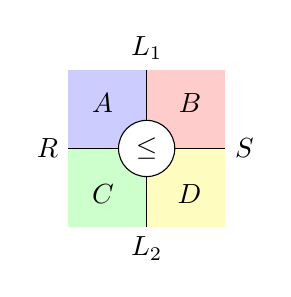
\begin{tikzpicture}[baseline]
    \path[fill=blue!20] rectangle (-1,1);
    \path[fill=red!20] rectangle (1,1);
    \path[fill=green!20] rectangle (-1,-1);
    \path[fill=yellow!25] rectangle (1,-1);
    \draw (0,0) -- (0,+1) node[anchor=south] {$L_1$};
    \draw (0,0) -- (+1,0) node[anchor=west] {$S$};
    \draw (0,0) -- (0,-1) node[anchor=north] {$L_2$};
    \draw (0,0) -- (-1,0) node[anchor=east] {$R$};
    \node[draw,circle,fill=white] (sim) {$\le$};
    \begin{scope}[inner sep=3mm]
      \node[below right] at (-1,1) {$A$};
      \node[below left] at (1,1) {$B$};
      \node[above right] at (-1,-1) {$C$};
      \node[above left] at (1,-1) {$D$};
    \end{scope}
  \end{tikzpicture}
  \quad \Rightarrow \quad
  \begin{tikzpicture}[baseline]
    \tikzset{to path={
        .. controls ($(\tikztostart)!\stens!(\tikztostart -| \tikztotarget)$)
        and ($(\tikztotarget)!\stens!(\tikztostart -| \tikztotarget)$) ..
        (\tikztotarget) \tikztonodes}}
  
    \path (-1, +1) coordinate (R1) node[above] {$\dagger R^*$};
    \path (+1, -1) coordinate (R2) node[below] {$\dagger R_*$};
    \path (0, +1) coordinate (L1) node[above] {$ \llbracket L_1 \rrbracket^\dagger $};
    \path (0, -1) coordinate (L2) node[below] {$ \llbracket L_2 \rrbracket^\dagger $};

    
    \fill[color=red!20] (sim) to (R2) -- (+1.2,-1) -- (+1.2,0) -- cycle;
    \path[fill=red!20] rectangle (+1.2,+1);
    \fill[color=green!20] (sim) to (R1) -- (-1.2,+1) -- (-1.2,0) -- cycle;
    \path[fill=green!20] rectangle (-1.2,-1);

    \fill[color=yellow!20] (sim) to (R2) -- (L2) -- cycle;
    \fill[color=yellow!20] (0,0) to (R2) -- (L2) -- cycle;
    \fill[color=blue!20] (sim) to (R1) -- (L1) -- cycle;
    \fill[color=blue!20] (0,0) to (R1) -- (L1) -- cycle;
    
    \node[draw,circle,fill=white] (sim) {$\sqsubseteq$};
    \node[below right] at (-0.9,+1) {$\dagger \llbracket A \rrbracket$};
    \node[below left] at (+1,+1) {$\dagger \llbracket B \rrbracket$};
    \node[above right] at (-1,-1) {$\dagger \llbracket C \rrbracket$};
    \node[above left] at (0.9,-1) {$\dagger \llbracket D \rrbracket$};
    
    \draw (sim) to (R1);
    \draw (sim) -- (L1);
    \draw (sim) to (R2);
    \draw (sim) -- (L2);
  \end{tikzpicture}
\]

\subsection{Control Operators (optional, medium difficulty)}

Although we can't define things like setjmp/longjmp/context switching
directly in terms of the CompCertO semantics,
we can define them as operators on embedded games semantics
of CompCert programs,
which interpret calls to the relevant primitives
in the appropriate way.
In this part we could for example:
\begin{itemize}
  \item Give a specification of context switching in these terms
  \item Give a certified implementation at the assembly level
\end{itemize}
This would go a long way towards
a reformulation of (parts of) CCAL into RBGS.

\subsection{Processes and their Environment (optional, lesser difficulty)}

Define \emph{loaders} to ``close'' the C interface of a component.
This means we don't have to deal with memory states any more
and just get the observable behavior of a closed process.
That behavior could have a degrees of sophistication:
\begin{itemize}
  \item Just use CompCert events, but use game semantics to interpret them
  \item Still allow outgoing calls in the (semi-)closed semantics
  \item Have the loader include semantics for some standard library functions,
    and give a higher-level view of what they do
    using a new outgoing language interface.
\end{itemize}

If we do that,
we can model how closed CompCert processes interact
with the operating system,
and could give a small example like
specify and verify simple versions of
the \texttt{sort} and \texttt{uniq} commands,
then model the behavior of a
\texttt{sort|uniq}
pipeline.

Another reason to do this would be to close a gap in CompCertO,
where currently we do not prove that the initial invocation of main
(including the initial memory state)
is compatible with our calling convention.

\section{Certified Abstraction Layers}

Certified abstraction layers can be embedded into the category of effect
signatures.

The signature of a layer interface or implementation
can be encoded as an effect signature.
For example:
\begin{align*}
  E_\kw{bq} &:= \{
    \kw{enq}[v] : \mathbbm{1}, \kw{deq} : V \mid
    v \in V \} \\
  E_\kw{rb} &:= \{
    \kw{set}[i, v] \! : \! \mathbbm{1},
    \kw{get}[i] \! : \! V,
    \kw{inc}_1 \! : \! \mathbb{N},
    \kw{inc}_2 \! : \! \mathbb{N} \! \mid \!
    i \in \mathbb{N}, v \in V \}
\end{align*}

In order to handle the layer's abstract data,
we can extend signatures with state in the following way:
\[
  E@S :=
    \{ m@k : \kw{ar}(m) \times S \mid
       m \in E, k \in S \}
\]

A layer interface $L$ with a signature $E$
and states in $S$
can be interpreted as
a homomorphism $\llbracket L \rrbracket : I \multimap E@S$.
Recall that a signature homomorphism of type $I \multimap E$
chooses arguments for each possible operation.
\[
  \llbracket L \rrbracket (m@k) :=
    \bigsqcup L.m@k
\]

We introduce a special homomorphism $e^k : \dagger E@S \multimap \dagger E$
to erase the explicit abstract state and instead use
strategies as specifications, where $k \in S$
is a state.
\[
  e^k(\underline{m}ns) \mathrel{:=} \bigsqcup_{k'\in S} \underline{m@k}(n@k' \mapsto e^{k'}(s))
\]
Given an initial state $k$, the embedded specification
in terms of the game model is defined as
\[
  \llbracket L \rrbracket^k \mathrel{:=} e^k \circ \llbracket L \rrbracket^\dagger : I \multimap \dagger E
\]

Given an underlay $L$ with signature $F$ and abstract state $S_2$
a layer implementation $M$
with an overlay signature $F$
extending the abstract state to $(S_1, S_2)$
can be interpreted as
a signature homomorphism $\llbracket M \rrbracket^m :  \dagger E@S_2 \multimap F@(S_1, S_2)$
by replacing external calls to underlay primitives
in the definition of $M$ with the corresponding operations:
\[
  \llbracket M \rrbracket^m \mathrel{:=} (M.m)[e \mathrel{:=} ???]
\]
The full behavior of implementation relies on
an underlay specification $I \multimap \dagger E$.
In order to compose them together
we introduce an adapter $\iota: E \multimap E@S$
that store the state upon an invocation of an operation to the underlay
and adjoin the same state to the next
incoming move.
\[
  \iota(m@k) \mathrel{:=} \underline{m}(n \mapsto n@k)
\]
Together with the state eraser,
a layer implementation $M$
given an initial state $k=(k_1,k_2)$
can be interpret as
\[
  \llbracket M \rrbracket^k \mathrel{:=}
  e^k \circ \llbracket M \rrbracket^\dagger \circ \dagger \iota : \dagger E \multimap \dagger F
\]
Consequently, running the implementation on top of
a underlay specification $L$ yield the composition
\[
  \llbracket M \rrbracket^{k_1,k_2} \circ \llbracket L \rrbracket^{k_2} : I \multimap \dagger F
\]
The layer judgment $L_1 \vdash_R M : L_2$,
which means that a layer implementation $M$
correctly implements $L_2$ on top of  $L_1$ through
a simulation relation $R \subseteq S_2 \times S_1$,
can then be interpreted as:
\[
  L_1 \vdash_R M : L_2 \Leftrightarrow
  \forall k_2\ R\ k_1\,.\, 
\llbracket L_2 \rrbracket^{k_2} \sqsubseteq
\llbracket M \rrbracket^{k_1} \circ \llbracket L \rrbracket^{\iota_2(k_1)}
\]
where $\iota_2$ is the projection to extract underlay state from $k_1$.

\newpage

\noindent
For now,
the rest of this document contains my previous CompCertOX write-up.

\begin{figure}[h] % fig:ex {{{
  \begin{center}
    \begin{tikzcd}[row sep=1cm, column sep=1.5cm]
      1 \ar[d, double, dash] \ar[rrr, ->>, "L''"] &&&
      \mathcal{C}@K''
        \ar[d, <->, "S"]
        \ar[r, ->>, "\llbracket C \rrbracket@K''"] &
      \mathcal{C}@K''
        \ar[ddd, <->, "R \circ S"]
      \\
      1 \ar[d, double, dash] \ar[rr, ->>, "L'"] &&
      \mathcal{C}@K'
        \ar[d, <->, "R"]
        \ar[r, ->>, "\llbracket N \rrbracket@K'"] &
      \mathcal{C}@K'
        \ar[d, <->, "R"]
      \\
      1 \ar[d, double, dash] \ar[r, ->>, "L"] &
      \mathcal{C}@K
        \ar[d, double, dash] 
        \ar[r, ->>, "\llbracket M \rrbracket@K"] &
      \mathcal{C}@K
        \ar[r, ->>, "\llbracket N \rrbracket@K"] &
      \mathcal{C}@K
        \ar[d, double, dash]
      \\
      1 \ar[d, double, dash] \ar[r, ->>, "L"] &
      \mathcal{C}@K
        \ar[d, double, dash] 
        \ar[rr, ->>, "\llbracket M + N \rrbracket@K"] &&
      \mathcal{C}@K
        \ar[r, ->>, "\llbracket C \rrbracket@K"] &
      \mathcal{C}@K
        \ar[d, double, dash] 
      \\
      1 \ar[r, ->>, "L"] &
      \mathcal{C}@K
        \ar[rrr, ->>, "\llbracket C + M + N \rrbracket@K"] &&&
      \mathcal{C}@K
    \end{tikzcd}
  \end{center}
  \caption}}

\section{Overview} %{{{

Our usual
\href{https://certikos.github.io/rbgs-papers/thesis/thesis.pdf\#chapter.4}%
  {theory of abstraction layers}
can be formulated in CompCertO's double category of
language interfaces, simulation conventions and transition systems:
\begin{itemize}
  \item A layer interface $L$ with abstract states in $K$
    is represented as $L : 1 \twoheadrightarrow \mathcal{C}@K$
  \item Clight semantics define
    $\llbracket M \rrbracket : \mathcal{C} \twoheadrightarrow \mathcal{C}$
    and lift to
    $\llbracket M \rrbracket @ K :
     \mathcal{C}@K \twoheadrightarrow \mathcal{C}@K$
  \item Abstraction relations define simulation conventions
    $R : \mathcal{C}@K' \Leftrightarrow \mathcal{C}@K$
  \item Layer correctness
    $L \vdash_R M : L'$
    is encoded as
    $L' \le_{\mathsf{id} \twoheadrightarrow R}
     \llbracket M \rrbracket @K \circ L$
\end{itemize}
\autoref{fig:ex}
demonstrates how these ingredients may fit together
in a typical situation.

The following operators
are used to formulate vertical and horizontal composition
of abstraction layers.
In the homogenous case
$(A \twoheadrightarrow A) \times
 (A \twoheadrightarrow A) \rightarrow
 (A \twoheadrightarrow A)$,
they under-approximate $\oplus$
and can therefore be implemented by linking.
\begin{itemize}
  \item Categorical composition \hfill
    $\circ :
      (B \twoheadrightarrow C) \times
      (A \twoheadrightarrow B) \rightarrow
      (A \twoheadrightarrow C) \qquad$
  \item Flat composition \hfill
    $\uplus :
      (A \twoheadrightarrow B) \times
      (A \twoheadrightarrow B) \rightarrow
      (A \twoheadrightarrow B) \qquad$
\end{itemize}
To reconnect formally with Yu's work,
we can investigate the following further:
\begin{itemize}
  \item A CompCertO transition system $L : A \twoheadrightarrow B$
    can be embedded into $\dagger A \multimap B$.
  \item The cliques of $\dagger \mathcal{C}$
    are universal abstract states.
  \item We can map between effect signatures $E$
    and the language interfaces $\mathcal{C}, \mathcal{A}$.
\end{itemize}
We can then define
a principled embedding
into game semantics or coherence spaces.

\paragraph{Status}

This draft should mostly be accurate,
however we will have to work out some of the details and kinks.
Here is a list of issues:
\begin{itemize}
  \item Components which make outgoing calls
    to functions in their own domain
    cause problems in the relationship between
    $\circ$, $\uplus$ and $\oplus$.
  \item In fact the word ``domain'' is somewhat confusing,
    more precisely it's a set of symbols
    that are reserved by the component.
\end{itemize}

%A certified abstraction layer
%$L_2 \vdash_R M : L_1$
%establishes that:
%\[
%  L_1 \le_{\mathsf{id} \twoheadrightarrow R}
%  \llbracket M \rrbracket @K_2 \circ L_2
%\]
%Various properties of the operators involved
%ensure that
%for any context $C$,
%\[
%  \llbracket C \rrbracket@K_1 \circ L_1
%  \: \le_{\mathsf{id} \twoheadrightarrow R} \:
%  \llbracket C \rrbracket@K_2 \circ \llbracket M \rrbracket@K_2 \circ L_2
%  \: \le_{\mathsf{id} \twoheadrightarrow \mathsf{id}} \:
%  \llbracket C + M \rrbracket@K_2 \circ L_2
%  \,.
%\]
%In particular,
%this enables vertical composition:
%\[
%  L_1
%  \: \le_{\mathsf{id} \twoheadrightarrow R} \:
%  \llbracket M \rrbracket@K_2 \circ L_2
%  \: \le_{\mathsf{id} \twoheadrightarrow S} \:
%  \llbracket M + N \rrbracket@K_3 \circ L_3
%\]
%On the other hand,
%the flat composition operator:
%\[
%  L_1, L_2 : A \twoheadrightarrow B
%  \vdash
%  L_1 \uplus L_2 : A \twoheadrightarrow B
%\]
%allows us to carry out a similar

%}}}

\section{Categorical structure of CompCertO semantics} %{{{

The semantic model used in CompCertO
can be organized into a double category:
\begin{itemize}
  \item the objects are language interfaces;
  \item the horizontal morphisms are open transition systems;
  \item the vertical morphisms are simulation conventions;
  \item the 2-cells are simulations.
\end{itemize}
The CompCertO paper defines
the vertical composition of simulation conventions,
but focuses on a symmetric form of horizontal composition,
meant to model linking:
\[
  {\oplus} :
    (A \twoheadrightarrow A) \times
    (A \twoheadrightarrow A) \rightarrow
    (A \twoheadrightarrow A)
\]

In this section,
I complement the constructions on CompCertO's open semantics
to make their double category structure explicit.
In particular,
I introduce the simpler and more fundamental
horizontal composition operators:
\[
  \begin{array}{c@{\:}l}
  {\circ} &:
    (B \twoheadrightarrow C) \times
    (A \twoheadrightarrow B) \rightarrow
    (A \twoheadrightarrow C)
  \\
  {\uplus} &:
    (A \twoheadrightarrow B) \times
    (A \twoheadrightarrow B) \rightarrow
    (A \twoheadrightarrow B)
  \end{array}
\]
The linking operator $\oplus$
can then be recovered or characterized as the fixed point
\[
  L_1 \oplus L_2 :=
    \mu X \cdot (L_1 \uplus L_2) \circ X
  \,.
\]

\subsection{Horizontal category} %{{{

\subsubsection{Identity} %{{{

The identity transition system $\mathsf{id}_A : A \twoheadrightarrow A$
can be defined as:
\[
  \mathsf{id}_A :=
    \langle A^\circ + A^\bullet,\: \varnothing,\: \varnothing,\: I,\: X,\: Y,\: F \rangle
\]
The components are defined by the rules:
\[
  \begin{prooftree}
    \infer0{q \mathrel{I} \iota_1(q)}
  \end{prooftree}
  \qquad
  \begin{prooftree}
    \infer0{\iota_1(q) \mathrel{X} q}
  \end{prooftree}
  \qquad
  \begin{prooftree}
    \infer0{r \mathrel{Y^{\iota_1(q)}} \iota_2(r)}
  \end{prooftree}
  \qquad
  \begin{prooftree}
    \infer0{\iota_2(r) \mathrel{F} r}
  \end{prooftree}
\]

%}}}

\subsubsection{Composition} %{{{

Suppose we have the transition systems:
\begin{align*}
  L_1 &= \langle S_1, {\rightarrow_1}, D_1, I_1, X_1, Y_1, F_1 \rangle
    : B \twoheadrightarrow C
  \\
  L_2 &= \langle S_2, {\rightarrow_2}, D_2, I_2, X_2, Y_2, F_2 \rangle
    : A \twoheadrightarrow B
\end{align*}
The composite transition system is defined as
\[
  L_1 \circ L_2 :=
  \langle S, {\rightarrow}, D_1 \cup D_2, I, X, Y, F \rangle
\]
with the following components.
States are of the form:
\[
    S := S_1 + (S_2 \times S_1)
\]
Initially, the environment question activates $L_1$:
\[
  \begin{prooftree}
    \hypo{q_C \mathrel{I_1} s_1}
    \infer1{q_C \mathrel{I} \iota_1(s_1)}
  \end{prooftree}
  \qquad
  \begin{prooftree}
    \hypo{s_1 \rightarrow_1 s_1'}
    \infer1{\iota_1(s_1) \rightarrow \iota_1(s_1')}
  \end{prooftree}
  \qquad
  \begin{prooftree}
    \hypo{s_1 \mathrel{F_1} r_C}
    \infer1{\iota_1(s_1) \mathrel{F} r_C}
  \end{prooftree}
\]
When an external call is encountered,
the question is used to activate $L_2$:
\[
  \begin{prooftree}
    \hypo{s_1 \mathrel{X_1} q_B}
    \hypo{q_B \mathrel{I_2} s_2}
    \infer2{\iota_1(s_1) \rightarrow \iota_2(s_2, s_1)}
  \end{prooftree}
\]
Execution proceeds according to $L_2$,
\[
  \begin{prooftree}
    \hypo{s_2 \rightarrow_2 s_2'}
    \infer1{\iota_2(s_2, s_1) \rightarrow \iota_2(s_2', s_1)}
  \end{prooftree}
  \qquad
  \begin{prooftree}
    \hypo{s_2 \mathrel{X_2} q_A}
    \infer1{\iota_2(s_2, s_1) \mathrel{X} q_A}
  \end{prooftree}
  \qquad
  \begin{prooftree}
    \hypo{r_A \mathrel{Y_2^{s_2}} s_2'}
    \infer1{r_A \mathrel{Y^{\iota_2(s_2, s_1)}} \iota_2(s_2', s_1)}
  \end{prooftree}
\]
until a final state of $L_2$ is reached,
at which point $L_1$ is resumed:
\[
  \begin{prooftree}
    \hypo{s_2 \mathrel{F_2} r_B}
    \hypo{r_B \mathrel{Y_1^{s_1}} s_1'}
    \infer2{\iota_2(s_2, s_1) \rightarrow \iota_1(s_1')}
  \end{prooftree}
\]

%}}}

\subsubsection{Properties} %{{{

I will write:
\begin{itemize}
  \item $L_1 \le L_2$
    to mean $L_1 \le_{\mathsf{id} \twoheadrightarrow \mathsf{id}} L_2$,
  \item $L_1 \equiv L_2$
    to mean $L_1 \le L_2 \wedge L_2 \le L_1$.
\end{itemize}
The expected properties of the horizontal
identity and categorical composition
can then be formulated in the following way.

\begin{theorem}
For a transition system $L : A \twoheadrightarrow B$,
the following property holds:
\[
    L \circ \mathsf{id}_A \equiv \mathsf{id}_B \circ L \equiv L
    \,.
\]
Moreover, for the transition systems
\[
  \begin{tikzcd}
    A \ar[r, ->>, "L_3"] &
    B \ar[r, ->>, "L_2"] &
    C \ar[r, ->>, "L_1"] &
    D \,,
  \end{tikzcd}
\]
the following property holds:
\[
    (L_1 \circ L_2) \circ L_3 \equiv L_1 \circ (L_2 \circ L_3)
\]
\begin{proof}
It should be straightforward to verify
that the identity acts as a unit for composition.
Associativity can be verified using
the simulation relation:
\[
  \begin{array}{rr}
    \hline
    L_1 \circ (L_2 \circ L_3) & (L_1 \circ L_2) \circ L_3 \\
    \hline
    \iota_1(s_1) & \iota_1(\iota_1(s_1)) \\
    \iota_2(\iota_1(s_2), s_1) & \iota_1(\iota_2(s_2, s_1)) \\
    \iota_2(\iota_2(s_3, s_2), s_1) & \iota_2(s_3, \iota_2(s_2, s_1)) \\
    \hline
  \end{array}
\]
\end{proof}
\end{theorem}

%}}}

\begin{remark}[Domains and categorical composition]
  Unlike the horizontal composition operator $\oplus$
  and the flat composition operator $\uplus$ introduced in the next section,
  categorical composition does not make use of the component's domains
  to compute the behavior of the composite transition system.
  This means that in general,
  a component may exhibit meaningful behaviors on queries outside its domain.
  This is the case in particular for $\mathsf{id}_A$,
  where the domain is $\varnothing$ but
  every possible query is associated with a behavior.
  In turn it suggests a modification to CompCertO's
  language semantics which would make them act as ``passthough''
  on queries outside of a module's domain.

  I should also note that categorical composition as
  given in this section will require modifying
  the definition of CompCertO's transition systems slightly.
  As it stands,
  a component's domain $D$ is a set of queries of
  the incoming language interface.
  However,
  for the domain $D_1 \cup D_2$ used in $L_1 \circ L_2$
  to make sense when $B \neq C$,
  we will have to change it to a language-independent
  notion of domain, for example a set of identifiers.
  Language interfaces
  would then provide a way to recognize whether queries
  are part of a domain expressed in this general way.
\end{remark}

%}}}

\subsection{Simulations} %{{{

Horizontal composition is compatible with simulations in the following sense.
Given
$L_1 : B \twoheadrightarrow C$ and $L_2 : A \twoheadrightarrow B$,
which are simulated respectively by
$L_1' : B' \twoheadrightarrow C'$ and $L_2' : A' \twoheadrightarrow B'$,
the following property holds:
\[
  \begin{prooftree}
    \hypo{L_1 \le_{S \twoheadrightarrow T} L_1'}
    \hypo{L_2 \le_{R \twoheadrightarrow S} L_2'}
    \infer2{L_1 \circ L_2 \le_{R \twoheadrightarrow T} L_1' \circ L_2'}
  \end{prooftree}
\]
Diagrammatically,
this allows us to paste simulations squares horizontally:
\[
  \begin{tikzcd}
    A \ar[r, ->>, "L_1"] \ar[d, <->, "R"] &
    B \ar[r, ->>, "L_2"] \ar[d, <->, "S"] &
    C \ar[d, <->, "T"] \\
    A' \ar[r, ->>, "L_1'"'] &
    B' \ar[r, ->>, "L_2'"'] &
    C'
  \end{tikzcd}
  \qquad \Longrightarrow \qquad
  \begin{tikzcd}
    A \ar[rr, ->>, "L_1 \circ L_2"] \ar[d, <->, "R"] &&
    C \ar[d, <->, "T"] \\
    A' \ar[rr, ->>, "L_1' \circ L_2'"'] &&
    C'
  \end{tikzcd}
\]

Note that the vertical composition of simulation squares
corresponds to the usual composition of simulations already given
in the CompCertO paper:
\[
  \begin{prooftree}
    \hypo{L_1 \le_{R \twoheadrightarrow S} L_2}
    \hypo{L_2 \le_{T \twoheadrightarrow U} L_3}
    \infer2{L_1 \le_{R \cdot T \twoheadrightarrow S \cdot U} L_3}
  \end{prooftree}
  \hspace{3em}
  \begin{tikzcd}
    A_1 \ar[r, ->>, "L_1"] \ar[d, <->, "R"] & B_1 \ar[d, <->, "S"] \\
    A_2 \ar[r, ->>, "L_2"] \ar[d, <->, "T"] & B_2 \ar[d, <->, "U"] \\
    A_3 \ar[r, ->>, "L_3"] & B_3
  \end{tikzcd}
  \quad
  \begin{tikzcd}[row sep=large]
    A_1 \ar[r, ->>, "L_1"] \ar[dd, <->, "R \cdot T"] & B_1 \ar[dd, <->, "S \cdot U"] \\ \\
    A_3 \ar[r, ->>, "L_3"] & B_3
  \end{tikzcd}
\]

One last observation is that the identity transition system
allows us to formulate the refinement of simulation conventions itself
as a simulation square.
There is a nice symmetry
with the refinement of transition systems:
\[
  \begin{tikzcd}[sep=tiny]
    A \ar[dd, double, dash, "\mathsf{id}_A"'] \ar[rr, ->>, "L_1"] &&
    B \ar[dd, double, dash, "\mathsf{id}_B"] \\
    & L_1 \le L_2 & \\
    A \ar[rr, ->>, "L_2"'] &&
    B
  \end{tikzcd}
  \hspace{5em}
  \begin{tikzcd}[sep=tiny]
    A \ar[dd, <->, "S"'] \ar[rr, double, dash, "\mathsf{id}_A"] &&
    A \ar[dd, <->, "R"] \\
    & R \sqsupseteq S & \\
    B \ar[rr, double, dash, "\mathsf{id}_B"'] &&
    B
  \end{tikzcd}
\]

%}}}

\subsection{Flat composition} %{{{

The categorical composition of two transition systems
chains them together,
directing any outgoing calls of the first
to incoming calls of the second.
I now introduce another kind of composition
which lays them out side-by-side.

\begin{definition}
The \emph{flat composition} of the transition systems
\begin{align*}
  L_1 &= \langle S_1, {\rightarrow_1}, D_1, I_1, X_1, Y_1, F_1 \rangle
    : A \twoheadrightarrow B
  \\
  L_2 &= \langle S_2, {\rightarrow_2}, D_2, I_2, X_2, Y_2, F_2 \rangle
    : A \twoheadrightarrow B
\end{align*}
is the transition system
$L_1 \uplus L_2 : A \twoheadrightarrow B$
defined as:
\[
  L_1 \uplus L_2 :=
    \langle
      S_1 + S_2, \:
      {\rightarrow}, \:
      D_1 \cup D_2, \:
      I, \: X, \: Y, \: F
    \rangle
\]
The components are defined by the following rules,
where $i \in \{1, 2\}$:
\[
  \begin{prooftree}
    \hypo{q \mathrel{I_i} s}
    \hypo{q \in D_i}
    \infer2{q \mathrel{I} \iota_i(s)}
  \end{prooftree}
  \quad
  \begin{prooftree}
    \hypo{s \rightarrow_i s'}
    \infer1{\iota_i(s) \rightarrow \iota_i(s')}
  \end{prooftree}
  \quad
  \begin{prooftree}
    \hypo{s \mathrel{X_i} q}
    \infer1{\iota_i(s) \mathrel{X} q}
  \end{prooftree}
  \quad
  \begin{prooftree}
    \hypo{r \mathrel{Y_i^s} s'}
    \infer1{r \mathrel{Y^{\iota_i(s)}} \iota_i(s')}
  \end{prooftree}
  \quad
  \begin{prooftree}
    \hypo{s \mathrel{F_i} r}
    \infer1{\iota_i(s) \mathrel{F} r}
  \end{prooftree}
\]
\end{definition}

\noindent
I suspect the following properties hold when applicable:
\begin{itemize}
  \item $\mathsf{id} \uplus L \equiv L \uplus \mathsf{id} \equiv L$
  \item $(L_1 \uplus L_2) \circ L \equiv (L_1 \circ L) \uplus (L_2 \circ L)$
\end{itemize}

\begin{remark}
It may be necessary for $\uplus$
to act as \emph{passthrough}
for queries outside of its domain.
This would enable the correspondence with $\oplus$
described in the next section.

The main difficulty is that
this can only be done when $A = B$,
so we would want to achieve this effect indirectly.
One option would be to expect language semantics
to be \emph{passthrough} outside their domain
and to have a nondeterministic choice between the components
when we're outside the domain of both.
That is to say,
each component is \emph{inhibited by the other's domain}
instead of \emph{enabled by its own}.
In normal situations the behavior of both components
would be the same in the ``gap'' between the domains,
so it would only be nondeterminism on a formal level.
\end{remark}

%}}}

\subsection{Linking} %{{{

The linking operator $\oplus$
can be described as the limit:
\[
  L_1 \oplus L_2 :=
  \bigvee_{n \in \mathbb{N}}
    (L_1 \uplus L_2)^n \circ \bot_{D_1 \cup D_2}
\]
where:
\begin{itemize}
  \item
    $L^n$ is the $n$-fold composition $L \circ \cdots \circ L$;
  \item
    $D_1$ and $D_2$ are the respective domains of $L_1$ and $L_2$;
  \item
    $\bot_D$ is undefined on its domain $D$ and
    \emph{passthrough} outside of it.
\end{itemize}
Note in particular that $\mathsf{id} \equiv \bot_\varnothing$.

For certified abstraction layers,
our main interest is that $\oplus$ can be used
to established a connexion between
the various kinds of transition system compositions
and the semantics of the linked program.

\begin{theorem}
For two Clight programs $M$ and $N$,
the linked program $M + N$ is a correct implementation of
$\llbracket M \rrbracket \oplus \llbracket N \rrbracket$:
\[
    \llbracket M \rrbracket \oplus \llbracket N \rrbracket \le
    \llbracket M + N \rrbracket
\]
\begin{proof}
A linking theorem for the Asm language has already been proved.
The Clight proof should be similar.
\end{proof}
\end{theorem}

Then the key fact is that $\circ$ and $\uplus$
are both under-approximations of $\oplus$;
in other words, they are both implemented by linking:
\begin{align*}
  \llbracket M \rrbracket \circ \llbracket N \rrbracket \: &\le \:
    \llbracket M \rrbracket \oplus \llbracket N \rrbracket \: \le \:
    \llbracket M + N \rrbracket \\
  \llbracket M \rrbracket \uplus \llbracket N \rrbracket \: &\le \:
    \llbracket M \rrbracket \oplus \llbracket N \rrbracket \: \le \:
    \llbracket M + N \rrbracket
\end{align*}
The first property in particular
can be visualized as the simulation square:
\begin{equation}
  \begin{tikzcd}
    \mathcal{C} \ar[r, "\llbracket N \rrbracket"] \ar[d, double, dash] &
    \mathcal{C} \ar[r, "\llbracket M \rrbracket"] &
    \mathcal{C} \ar[d, double, dash] \\
    \mathcal{C} \ar[rr, "\llbracket M + N \rrbracket"'] & &
    \mathcal{C}
  \end{tikzcd}
  \label{eqn:linkingsquare}
\end{equation}

%}}}

\subsection{String diagrams} %{{{

Like 2-categories,
double categories admit a string diagram calculus where:
\begin{itemize}
  \item objects are represented by regions,
  \item horizontal morphisms are represented by vertical lines,
  \item vertical morphisms are represented by horizontal lines,
  \item 2-cells are represented by points.
\end{itemize}

The diagrams I have drawn so far
efficiently convey the type structure of the semantic framework;
they describe
the way language interfaces,
transition systems and simulation conventions
compose and interact.
But the \emph{simulation proofs} themselves
are literally found in the \emph{gaps} between
these entities.

String diagrams are useful because they turn this hierarchy on its head,
and offer a compelling visualization of the ways
complex simulations can be assembled from simpler ones.
A basic simulation square $f \le_{R \twoheadrightarrow S} g$ is drawn as:
\[
  \begin{tikzcd}[sep=small]
    A \ar[rr, ->>, "f"] \ar[dd, <->, "R"'] &&
    B \ar[dd, <->, "S"] \\
    & \phi & \\
    C \ar[rr, ->>, "g"'] &&
    D
  \end{tikzcd}
  \qquad \qquad
  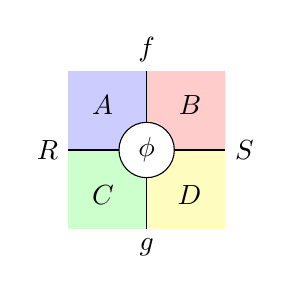
\begin{tikzpicture}[baseline]
    \path[fill=blue!20] rectangle (-1,1);
    \path[fill=red!20] rectangle (1,1);
    \path[fill=green!20] rectangle (-1,-1);
    \path[fill=yellow!25] rectangle (1,-1);
    \draw (0,0) -- (0,+1) node[anchor=south] {$f$};
    \draw (0,0) -- (+1,0) node[anchor=west] {$S$};
    \draw (0,0) -- (0,-1) node[anchor=north] {$g$};
    \draw (0,0) -- (-1,0) node[anchor=east] {$R$};
    \node[draw,circle,fill=white] (sim) {$\phi$};
    \begin{scope}[inner sep=3mm]
      \node[below right] at (-1,1) {$A$};
      \node[below left] at (1,1) {$B$};
      \node[above right] at (-1,-1) {$C$};
      \node[above left] at (1,-1) {$D$};
    \end{scope}
  \end{tikzpicture}
\]

Much information can be elided from string diagrams.
Identity transition systems and simulation conventions
can be omitted completely.
Objects can be associated with a color,
eliminating redundant labeling.
For example,
here are depictions of
a simulation convention refinement property ($R \sqsupseteq S$),
a transition system refinement property ($L_1 \le L_2$),
and of the linking property (\ref{eqn:linkingsquare}):
\[
  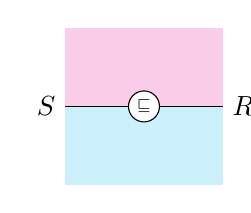
\begin{tikzpicture}[baseline]
    \path[fill=magenta!20] (-1,1) rectangle (1,0);
    \path[fill=cyan!20] (-1,0) rectangle (1,-1);
    \draw (-1,0) node[left] {$S$}
      -- (0,0) node[draw,circle,fill=white,inner sep=0.5mm] {\tiny $\sqsubseteq$}
      -- (1,0) node[right,overlay] {$R$};
  \end{tikzpicture}
  \qquad \qquad
  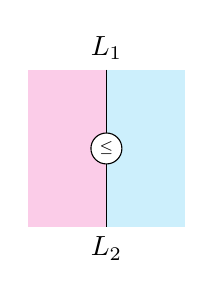
\begin{tikzpicture}[baseline]
    \path[fill=magenta!20] (-1,1) rectangle (0,-1);
    \path[fill=cyan!20] (0,1) rectangle (1,-1);
    \draw (0,1) node[above] {$L_1$}
      -- (0,0) node[draw,circle,fill=white,inner sep=0.5mm] {\tiny $\le$}
      -- (0,-1) node[below] {$L_2$};
  \end{tikzpicture}
  \qquad \qquad
  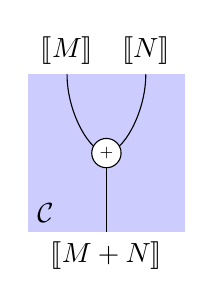
\begin{tikzpicture}[baseline]
    \path[fill=blue!20] (-1,-1) rectangle (1,1);
    \begin{scope}
      \draw (-0.5, +1) node[above] {$\llbracket M \rrbracket$}
        .. controls +(-90:0.5) and +(180:0.2) .. (0,0);
      \draw (+0.5, +1) node[above] {$\llbracket N \rrbracket$}
        .. controls +(-90:0.5) and +(0:0.2) .. (0,0);
      \draw (0,0) -- (0,-1) node[below] {$\llbracket M + N \rrbracket$};
    \end{scope}
    \node[draw,circle,fill=white,inner sep=0.5mm] {\tiny $+$};
    \node[above right] at (-1,-1) {$\mathcal{C}$};
  \end{tikzpicture}
\]

\noindent
Skipping ahead,
here is a string diagram rendition of \autoref{fig:ex}.
\[
  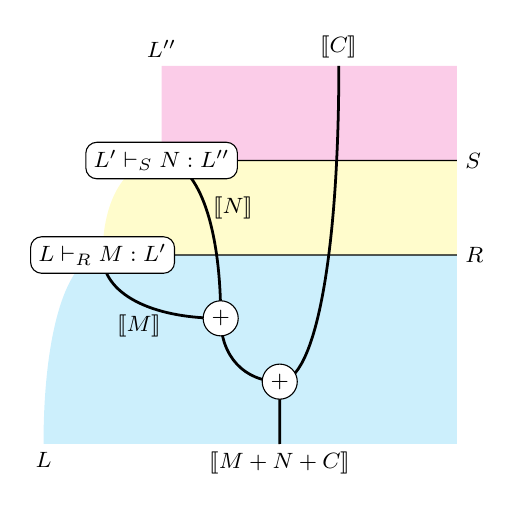
\begin{tikzpicture}[baseline,yscale=1.2,xscale=1.5]
    \footnotesize
    \tikzset{to path={
      .. controls ($(\tikztostart)!\stens!(\tikztostart -| \tikztotarget)$)
              and ($(\tikztotarget)!\stens!(\tikztostart -| \tikztotarget)$) ..
      (\tikztotarget) \tikztonodes}}

    % Boundary labels
    \begin{scope}
      \path (1,4) coordinate (L2) node[above] {$L''$};
      \path (2.5,4) coordinate (C) node[above] {$\llbracket C \rrbracket$};
      \path (3.5,3) coordinate (S) node[right] {$S$};
      \path (3.5,2) coordinate (R) node[right] {$R$};
      \path (0,0) coordinate (L) node[below] {$L$};
      \path (2,0) coordinate (T) node[below] {$\llbracket M+N+C \rrbracket$};
    \end{scope}

    % Simulation proofs
    \begin{pgfonlayer}{nodes}
      % Layer correctness
      \tikzset{every node/.style={rounded corners,draw,fill=white,inner sep=1mm}}
      \path (1,3) coordinate (LC2) node {$L' \vdash_S N : L''$};
      \path (0.5,2) coordinate (LC1) node {$L \vdash_R M : L'$};
      % Linking
      \tikzset{every node/.style={circle,draw,fill=white,inner sep=0.5mm}}
      \path (1.5,1.33) coordinate (LK1) node {$+$};
      \path (2,0.66) coordinate (LK2) node {$+$};
      % Parametricity
      \tikzset{every node/.style={circle,draw,fill=black,inner sep=0.5mm}}
      %\node (P2) at (4,2) {};
      %\node (P3) at (3,2) {};
    \end{pgfonlayer}

    % Regions
    \fill[color=magenta!20] (L2) to (LC2) -- (S) |- cycle;
    \fill[color=yellow!20] (LC2) to (LC1) -- (R) |- cycle;
    \fill[color=cyan!20] (LC1) to (L) -| (R) -- cycle;

    % Transition systems
    \begin{scope}[line width=1pt,inner sep=0.2mm]
      % \draw (L2) to (LC2) to node[above left,pos=0.75] {$L'$} (LC1) to (L);
      \draw (T) to (LK2) to (LK1) to node[below left,pos=0.3] {$\llbracket M \rrbracket$} (LC1);
      \draw (LC2) to node[above right,pos=0.6] {$\llbracket N \rrbracket$} (LK1);
      \draw (LK2) to (C);
    \end{scope}

    % Simulation conventions
    \begin{scope}
      \draw (LC2) to (S);
      \draw (LC1) to (R);
    \end{scope}

    % Region labels
%    \begin{scope}[opacity=0.4]
%      \node[below right] at (-0.5,1) {$1$};
%      \node[above left] at (4,0) {$K$};
%      \node[left] at (4,3.5) {$K'$};
%      \node[below left] at (4,5) {$K''$};
%    \end{scope}
  \end{tikzpicture}
\]
Here the white region corresponds to
the empty language interface $1$,
whereas the colored regions correspond to
a version of the $\mathcal{C}$ language interface
extended to carry the various kinds of abstract states
used by the layer interfaces $L$, $L'$ and $L''$.
From the outer boundary of the diagram,
we can read the simulation property
\[
  \llbracket C \rrbracket@K'' \circ L''
  \le_{1 \twoheadrightarrow S \cdot R}
  \llbracket M + N + C \rrbracket@K \circ L
  \,.
\]
The diagram is a proof of this property,
constructed from the following components:
\begin{itemize}
  \item Layer correctness properties of the form
    \[
      L' \le_{\mathsf{id} \twoheadrightarrow R} \llbracket M \rrbracket@K \circ L
      \,,
    \]
    depicted as rectangular boxes.
  \item The linking property (\ref{eqn:linkingsquare}),
    lifted to operate with abstract state
    \[
      \llbracket M \rrbracket@K \circ \llbracket N \rrbracket@K
      \le_{\mathsf{id} \twoheadrightarrow \mathsf{id}}
      \llbracket M + N \rrbracket@K
      \,,
    \]
    depicted with a plus symbol.
  \item The compatibility of language semantics with abstraction relations
    \[
      \llbracket C \rrbracket@K'
      \le_{R \twoheadrightarrow R}
      \llbracket C \rrbracket@K
      \,,
    \]
    depicted as crossings between the horizontal lines ($R$)
    and vertical lines ($\llbracket C \rrbracket$).
\end{itemize}

%}}}

%}}}

\section{Certified abstraction layers} %{{{

I will use the notations and concepts outlined in
\href{https://certikos.github.io/rbgs-papers/thesis/thesis.pdf\#chapter.4}{Chapter 4}
of my thesis.
In particular,
\href{https://certikos.github.io/rbgs-papers/thesis/thesis.pdf#section.4.4}{\S 4.4}
reframes our CompCertX-based approach
into our more abstract formalism
and is a starting point for the following definitions.

\subsection{Abstract states} %{{{

In CompCertX,
the memory model is extended with an \emph{abstract state} component
which is used to specify the behavior of underlay primitives.

To extend CompCertO in a similar way,
given a set $K$ of abstract states,
we can introduce an operator to transform the language interface $A$
into the language interface $A@K$
where every question and answer
is annotated with an element of $K$.

\begin{definition}
For a language interface
$A = \langle A^\circ, A^\bullet \rangle$
we define the language interface:
\[
    A@K := \langle A^\circ \times K, \: A^\bullet \times K \rangle
    \,.
\]
\end{definition}

Then,
a transition system $L : A \twoheadrightarrow B$
can be lifted to $L@K : A@K \twoheadrightarrow B@K$,
which maintains an abstract state component
and threads it through the computation.

\begin{definition}
For a transition system
$L = \langle S, {\rightarrow}, D, I, X, Y, F \rangle$,
we define:
\[
    L@K \: := \:
      \langle S \times K, \: {\rightarrow} \times {=}_K, \:
            D \times K, \: I \times {=}_K, \: X \times {=}_K, \:
            Y_K, \: F \times {=}_K \rangle
\]
where the relation $Y_K$ is defined by the rule:
\[
  \begin{prooftree}
    \hypo{n \mathrel{Y^s} s'}
    \infer1{n@{k'} \mathrel{Y_K^{s@k}} s'@k'}
  \end{prooftree} 
\]
\end{definition}

Most of the relations involved in $L@K$
simply thread this component through unchanged (${-} \times {=}_K$).
At external calls,
we update the abstract state with
its value in the environment's answer.

A similar construction can be carried out for simulation conventions.

\begin{definition}
For a simulation convention $\mathbb{R} : A \leftrightarrow B$
with $\mathbb{R} = \langle W, \mathbb{R}^\circ, \mathbb{R}^\bullet \rangle$,
we define the simulation convention
$\mathbb{R}@K : A@K \leftrightarrow B@K$
in the following way:
\[
  \mathbb{R}@K \: := \:
    \langle
      W, \:
      \mathbb{R}^\circ \times {=}, \:
      \mathbb{R}^\bullet \times {=}
    \rangle
\]
\end{definition}

Together,
these definitions define a \emph{double endofunctor}
on the double category of
transition systems, simulation conventions and simulations.
The corresponding properties
are given as follows.

\begin{theorem}
  For the transition systems
  $L_1 : A \twoheadrightarrow B$ and
  $L_2 : B \twoheadrightarrow C$,
  we have:
  \[
    \mathsf{id}_A@K \equiv \mathsf{id}_{A@K}
    \qquad
    (g \circ f)@K \equiv g@K \circ f@K
  \]
  For the simulation conventions
  $R : A \leftrightarrow B$ and $S : B \leftrightarrow C$,
  we have:
  \[
    \epsilon_A@K \equiv \epsilon_{A@K}
    \qquad
    (R \cdot S)@K \equiv R@K \cdot S@K
  \]
  Finally,
  extending with abstract state preserves simulation squares:
  \[
    \begin{tikzcd}[row sep=large,column sep=large]
      A_1 \ar[r, ->>, "L_1"] \ar[d, <->, "R_A"'] &
      B_1 \ar[d, <->, "R_B"] \\
      A_2 \ar[r, ->>, "L_2"'] & B_2
    \end{tikzcd}
    \quad \Longrightarrow \quad
    \begin{tikzcd}[row sep=large, column sep=large]
      A_1@K \ar[r, ->>, "L_1@K"] \ar[d, <->, "R_A@K"'] &
      B_1@K \ar[d, <->, "R_B@K"] \\
      A_2@K \ar[r, ->>, "L_2@K"'] & B_2@K
    \end{tikzcd}
  \]
\end{theorem}

These properties essentially mean that
entire simulation diagrams
can be extended with abstract states at once.
For example,
if the following simulations hold:
\[
  \begin{tikzcd}[sep=large]
    A \ar[r, ->>, "f"] \ar[d, <->, "R"] &
    B \ar[r, ->>, "g"] &
    C \ar[r, ->>, "h"] \ar[d, <->, "S"] &
    D \ar[dd, <->, "T"]
    \\
    E \ar[rr, ->>, "x"] \ar[d, <->, "U"] &&
    F \ar[d, <->, "V"] &
    \\
    X \ar[rr, ->>, "\phi"] &&
    Y \ar[r, ->>, "\psi"] &
    Z
  \end{tikzcd}
\]
then we can conclude that the following simulations hold as well:
\[
  \begin{tikzcd}[row sep=large]
    A@K \ar[r, ->>, "f@K"] \ar[d, <->, "R@K"] &
    B@K \ar[r, ->>, "g@K"] &
    C@K \ar[r, ->>, "h@K"] \ar[d, <->, "S@K"] &
    D@K \ar[dd, <->, "T@K"]
    \\
    E@K \ar[rr, ->>, "x@K"] \ar[d, <->, "U@K"] &&
    F@K \ar[d, <->, "V@K"] &
    \\
    X@K \ar[rr, ->>, "\phi@K"] &&
    Y@K \ar[r, ->>, "\psi@K"] &
    Z@K
  \end{tikzcd}
\]
This will be especially useful for lifting
properties established in CompCertO
to the context of certified abstraction layers,
allowing for example versions of the
compiler correctness or linking properties
extended to include abstract state:
\[
  \begin{tikzcd}[row sep=large, column sep=huge]
    \mathcal{C}@K
      \ar[r, ->>, "\llbracket M \rrbracket@K"]
      \ar[d, <->, "\mathbb{C}@K"'] &
    \mathcal{C}@K
      \ar[d, <->, "\mathbb{C}@K"] \\
    \mathcal{A}@K
      \ar[r, ->>, "\llbracket C(M) \rrbracket@K"'] &
    \mathcal{A}@K
  \end{tikzcd}
  \qquad
  \begin{tikzcd}[sep=large]
    \mathcal{C}@K
      \ar[r, ->>, "\llbracket M \rrbracket@K"]
      \ar[d, double, dash] &
    \mathcal{C}@K
      \ar[r, ->>, "\llbracket N \rrbracket@K"] &
    \mathcal{C}@K
      \ar[d, double, dash] \\
    \mathcal{C}@K
      \ar[rr, ->>, "\llbracket M + N \rrbracket@K"'] &&
    \mathcal{C}@K
  \end{tikzcd}
\]


%}}}

\subsection{Layer interfaces} %{{{

Per the definitions in my thesis and our LICS'20 paper,
a layer interface can be described as a family of specifications:
\[
    \sigma^m : K \rightarrow \mathcal{P}^1(N \times K)
\]
where $(m \mathbin: N) \in E$ is an operation of the layer's signature.
In the case of the $\mathcal{C}$ language interface of CompCertO,
operations are of the form:
\[
    f(\vec{v}) : \mathsf{val}
    \qquad
    \text{where}
    \qquad
    f \in \mathsf{val}
    \qquad
    \vec{v} \in \mathsf{val}^*
\]

A layer interface specified in this style
can easily be represented as a CompCertO transition system
$\hat{\sigma} : 1 \twoheadrightarrow \mathcal{C}@K$,
defined as:
\[
  \hat{\sigma} := \langle
    \mathsf{val} \times \mathsf{mem} \times K,
    \varnothing,
    D,
    I,
    \varnothing,
    \varnothing,
    F
  \rangle
\]
A call into this transition system involves a single state.
At invocation,
we immediately query $\sigma$ to obtain the call's outcome
and save it in the transition system's state:
\[
  \begin{prooftree}
    \hypo{\sigma^{f(\vec{v})}(k) \ni (v', k')}
    \infer1{f(\vec{v})@m@k \mathrel{I} (v', m, k')}
  \end{prooftree}
\]
This single state admits no transition but is immediately final:
\[
  \begin{prooftree}
    \infer0{(v', m, k') \mathrel{F} v'@m@k'}
  \end{prooftree}
\]

The domain $D$ has to be specified in addition to $\sigma$,
which does not carry this information.
Alternatively,
we could use a more sophisticated embedding,
where $\sigma$ is defined in terms of a more abstract
effect signature $E$,
and where we specify a correspondance between
the operations of $E$ and $\mathcal{C}$ calls.

Using the definitions above,
the semantics of a Clight program $M$
on top of a layer interface
$L : 1 \twoheadrightarrow \mathcal{C}@K$
can be given as
\[
  \llbracket M \rrbracket @K \circ L \: : \:
  1 \twoheadrightarrow \mathcal{C}@K
  \,.
\]

%}}}

\subsection{Abstraction relations} %{{{

In CompCertX-based CertiKOS,
the abstraction relation between
an overlay with abstract states in $K_1$ and
an underlay with abstract states in $K_2$
is given as a pair of relations:
\[
  R^\mathsf{r} \subseteq K_1 \times K_2
  \qquad
  R^\mathsf{m} \subseteq K_1 \times \mathsf{mem}
\]
We also associate with each layer a set of global variables $G$
such that:
\[
  \begin{prooftree}
    \hypo{k_1 \mathrel{R^\mathsf{r}} m_2}
    \hypo{m_2 \cong_G m_2'}
    \infer2{k_1 \mathrel{R^\mathsf{r}} m_2'}
  \end{prooftree}
\]
where $\cong_G$ denotes the usual $\mathsf{Mem.unchanged\_on}$
relationship asserting that the two memories
associate the same contents to the global variables in $G$.

In CompCertO,
we can use these relations to define a
memory-extension-based simulation convention
$R : \mathcal{C}@K_1 \Leftrightarrow \mathcal{C}@K_2$
which captures CertiKOS-style abstraction between
overlay and underlay behaviors:
\begin{gather*}
 {\begin{prooftree}
    \hypo{k_1 \mathrel{R^\mathsf{r}} k_2}
    \hypo{k_1 \mathrel{R^\mathsf{m}} m_2}
    \hypo{m_1 \le_\mathsf{m} m_2}
    \hypo{m_1 \mathrel\text{no-perms-on} G}
    \hypo{\vec{v}_1 \le_\mathsf{v} \vec{v}_2}
    \infer5{f(\vec{v}_1)@m_1@k_1 \mathrel{R^\circ} f(\vec{v}_2)@m_2@k_2}
  \end{prooftree}}
\\[1em]
 {\begin{prooftree}
    \hypo{k_1 \mathrel{R^\mathsf{r}} k_2}
    \hypo{k_1 \mathrel{R^\mathsf{m}} m_2}
    \hypo{m_1 \le_\mathsf{m} m_2}
    \hypo{m_1 \mathrel\text{no-perms-on} G}
    \hypo{v'_1 \le_\mathsf{v} v'_2}
    \infer5{v'_1@m_1@k_1 \mathrel{R^\bullet} v'_2@m_2@k_2}
  \end{prooftree}}
\end{gather*}
Then we can
formulate the layer correctness property
$L \vdash_R M : L'$ as
\[
    L' \le_{\mathsf{id} \twoheadrightarrow R}
    \mathsf{Clight}(M)@K \circ L
    \,.
\]

%}}}

%}}}

\section{Coherence spaces} %{{{

%}}}

\section{Effect signatures} %{{{

%}}}

\section*{Interaction Specification Algebras} %{{{

[I am giving up on this section.
It is not really required for the main points the paper makes
and it is challenging to articulate everything in that context.
I will just review interaction specifications
in the main ideas section
and write another paper on algebraic game semantics.]

\begin{color}{gray}
[Briefly describe the LICS'20 model
for the sake of being self-contained.
Ideally, provide a characterization
as a free monad of some kind,
but this seems to be challenging.]

The work presented in this paper
builds on the \emph{interaction specification} model
of certified abstraction layers \cite{lics20}.
In this section,
we give a proper categorical characterization
of this model as a free monad,
which provides reasoning principles for
interaction specifications
independent of the particular construction
used to defined them.

\subsection{Overview} %{{{

The \emph{free monad} construction \cite{freemon}
has important applications in programming language semantics.
In particular,
it provides a bridge between
the traditional monadic approach
to modeling computational side-effect \cite{moggi}
and the constructions and techniques of universal algebra.
While monads in general do not compose easily,
algebraic theories enjoy a rich and uniform
composition framework.
By characterizing monads in terms of
the algebraic theories that induce them,
we can take advantage of this framework.

Recent work also connects the algebraic approach
to game semantics.
For simple games,
the traditional strategy construction
can be characterized as an initial algebra
in the category of
directed-complete partial orders and
strict Scott-continuous functions \cite{act21}.
Likewise,
the \emph{interaction specification} model
used as a starting point for our work
is inspired by both
game semantics and
algebraic effects.
However,
while \citet{lics20} presents its interaction specification monad
as a variation on the traditional free monad construction,
it does not provide a formal account of this assessment.

In this section,
we give a presentation of
the interaction specification monad
as a free monad.
This establishes the algebraic basis for the model,
and a more principled approach to inductive proofs.

%}}}

\subsection{Free Monad}

\subsection{Completely Distributive Lattices} %{{{

It is well-understood that
semi-lattices provide the algebraic foundation
of traditional nondeterminism.
Completely distributive lattices
provide a similar foundation for
dual nondeterminism with arbitrary angelic and demonic choices.

\begin{definition}
A \emph{complete lattice}
is a partially ordered set $\langle L, {\le} \rangle$
with all joins and meets.
This means in particular that $L$
has a least element $\bot = \bigvee \varnothing = \bigwedge L$
and a greatest element $\top = \bigwedge \varnothing = \bigvee L$.
A \emph{completely distributive} lattice
is a complete lattice which satisfies
the (equivalent) distributivity properties:
\begin{gather} \label{eqn:compdist}
  \bigvee_{i \in I} \bigwedge_{j \in J_i} x_{ij} =
  \bigwedge_{f \in \prod_i J_i} \bigvee_{i \in I} x_{i,f_i}
  \\
  \bigwedge_{i \in I} \bigvee_{j \in J_i} x_{ij} =
  \bigvee_{f \in \prod_i J_i} \bigwedge_{i \in I} x_{i,f_i}
\end{gather}
\end{definition}

These properties admit an intuitive game-theoretic interpretation.
Suppose the elements of $L$
are \emph{payoffs} in a zero-sum, two-player games
where the proponent and opponent
take turns making moves.
The proponent seeks to minimize the payoff.
If they can choose among the payoffs $(x_i)_{i \in I}$,
the outcome will be $\bigwedge_i x_i$.
Conversely,
if the opponent can choose among $(y_j)_{j \in J}$,
the outcome will be $\bigvee_j y_j$.
Hence the expression
$\bigwedge_i \bigvee_j x_{ij}$
denotes the result of a game where
the proponent first makes a choice $i \in I$,
the opponent then chooses $j \in J_i$,
producing the outcome $x_{ij}$.

We can reverse the order of these moves
by having the opponent play first
and choose a strategy $f \in \prod_i J_i$.
The proponent then selects $i \in I$,
leading to the outcome is $x_{i,f_i}$.
At first glance,
this game is very different:
the proponent has access to much more information
and can make a decision based on the opponent's choice of strategy.
However,
the expressions $\bigwedge_i \bigvee_j x_{ij}$
and $\bigvee_f \bigwedge_i x_{i,f_i}$
are only concerned with the case where both players adopt
an optimal strategy.
In this particular scenario,
the opponent choices were in effect already known,
hence the proponent gains no advantage.

%}}}

\subsection{Multimorphisms of Complete Lattices}

In $\mathbf{Set}$,
where we can reason about fully defined,
terminating programs,
notion of algebra so signature is easy:
\[
    \alpha : \sum_m \prod_n A \rightarrow A
\]
In other words,
for each operation $(m : N) \in E$
we give a function $\alpha^m : A^N \rightarrow A$,
which gives the interpretation of a computation
invoking the effect $m$
with the possible continuations $(k_n)_{n \in N} \in A^N$.

\subsection{Tensor Products}

Tensor products in $\mathbf{CDLat}$
are difficult to pin down.
In particular,
there is no such thing as a \emph{bicomplete} homomorphism
of non-trivial complete lattices,
since the required properties:
\begin{align*}
  f \left( \bigsqcap_{i \in I} x_i, y \right) &=
    \bigsqcap_{i \in I} f(x_i, y) &
  f \left( \bigsqcup_{i \in I} x_i, y \right) &=
    \bigsqcup_{i \in I} f(x_i, y) \\
  f \left( x, \bigsqcap_{i \in I} y_i \right) &=
    \bigsqcap_{i \in I} f(x, y_i) &
  f \left( x, \bigsqcup_{i \in I} y_i \right) &=
    \bigsqcup_{i \in I} f(x, y_i)
\end{align*}
are contradictory---%
consider for example $f(\bot, \top)$.

Explain how demonic choices must distribute
over environment choice of argument,
vs. angelic choices just move as in $\prod A_i \rightarrow A$.

\subsection{Interaction Algebras}

\subsection{Interaction Specifications}

\end{color}

\section{CompCertO stuff from my thesis}

[Explain how we can embed CompCertO semantics
for the purpose of CAL:
categorical/layered composition only,
don't care about footprints until the end,
angelic interpretation.]

In its strongest form,
the compiler correctness theorem proved in CompCert
is expressed as a forward simulation of labeled transition systems.
This simulation is then used to derive
a trace containment property.

Although CompCertO provides an updated notion of forward simulation,
in the compositional setting
it is challenging to
formulate a theorem analogous to trace containment.
To do so,
we must incorporate component interactions
into event traces.
Traces then become typed in the same way our transition systems are.
Because they include internal notions of state and interaction
which differ between the source and target languages,
the corresponding traces are no longer directly comparable,
and we must bring simulation conventions into the picture.

This is challenging because
simulation conventions involve
\emph{dual} nondeterminism:
both the system and the environment contribute choices
which determine how C-level behavior is realized at the assembly level.
Because of this,
neither trace inclusion (angelic nondeterminism)
nor trace containment (demonic nondeterminism)
are sufficient to express the relationship
between these behaviors.

\emph{Refinement-based game semantics} \cite{koenig20}
offers a solution,
in the form of a relatively simple game model
with full support for both angelic and demonic choices.
We have mechanized this model in the Coq proof assistant.
In this section,
we demonstrate how the compositional semantics used in CompCertO
can be interpreted in this setting.

%% preamble {{{
%
%The semantics of CompCert languages
%are given in terms of a simple notion of process behavior.
%By \emph{process}, I mean a self-contained computation
%which can be characterized by
%the sequence of system calls it performs.
%%Several steps are involved to go
%%from a source program to an executing process;
%%these steps are modeled by CompCert
%%with varying degrees of sophistication and accuracy.
%For a C program to be executed as a process,
%its translation units must be compiled to object files,
%then linked together
%into an executable binary
%loaded by the system.
%
%\begin{figure} % fig:process {{{
%  \centering
%    \begin{tikzpicture}[scale=1.25]
%        \tt
%        \node (Ms) at (1.5, 1) {whole-program.s};
%        \node (M1c) at (0, 3) {M1.c};
%        \node (M2c) at (1, 3) {M2.c};
%        \node (etc) at (2, 3) {\ldots};
%        \node (Mnc) at (3, 3) {M$n$.c};
%        \node (M1s) at (0, 2) {M1.s};
%        \node (M2s) at (1, 2) {M2.s};
%        \node (ets) at (2, 2) {\ldots};
%        \node (Mns) at (3, 2) {M$n$.s};
%        \draw (M1c) edge[->] (M1s);
%        \draw (M2c) edge[->] (M2s);
%        \draw (Mnc) edge[->] (Mns);
%        \draw (M1s) edge[->] (Ms);
%        \draw (M2s) edge[->] (Ms);
%        \draw (Mns) edge[->] (Ms);
%        \rm
%        \node at (-1.3, 2.5) {Compilation};
%        \node at (-1.3, 1.5) {Linking};
%
%        %\node (Mb) at (1.5, 0) {Running process};
%        %\node at (-1.3, 0.5) {Loading};
%        %\draw (Ms) edge[->] (Mb);
%
%        %\tt
%        %\node (Mc) at (1.5, 4) {whole-program.c};
%        %\draw (M1c) edge[->,dotted] (Mc);
%        %\draw (M2c) edge[->,dotted] (Mc);
%        %\draw (Mnc) edge[->,dotted] (Mc);
%    \end{tikzpicture}
%    \caption{CompCert's approximation of the C toolchain}
%    \label{fig:process}
%\end{figure}
%%}}}
%
%%Finally, the system loads the executable into memory
%%where initialization code sets up the process
%%and invokes the program's \texttt{main} function.
%%Since CompCert is a compiler from C to assembly,
%%but does not include an assembler or linker,
%The model used for verifying CompCert accounts for this
%in the way depicted in Figure~\ref{fig:process}.
%%The lowest-level objects considered
%%are CompCert \kw{Asm} programs.
%Linking is approximated by
%merging programs, seen as sets of global definitions.
%The execution
%of a program composed of the translation units
%$\texttt{M1.c} \ldots \texttt{M$n$.c}$
%which compile to
%$\texttt{M1.s} \ldots \texttt{M$n$.s}$
%is modeled as:
%\[
%    L_\kw{tgt} :=
%    \kw{Asm}[\texttt{M1.s} +
%             \cdots +
%             \texttt{M$n$.s}] \,.
%\]
%Here,
%$+$ denotes CompCert's linking operator and
%$\kw{Asm}$ maps an assembly program to its semantics.
%Note that the loading process is encoded
%as part of the definition of $\kw{Asm}$,
%which constructs a global environment
%laying out the program's code and static data
%into the runtime address space,
%and models the conventional invocation of \texttt{main}.
%To formulate compiler correctness,
%we must also specify the behavior of the source program.
%To this end,
%CompCert defines a linking operator
%and semantics
%for the language $\kw{Clight}$,%
%\footnote{
%  Although CompCert features a frontend for a richer version
%  of the C language,
%  the simplified intermediate dialect \kw{Clight}
%  is usually used as the source language
%  when using CompCert to build certified artifacts.
%  %In particular it is the target language of the
%  %\texttt{clightgen} utility which
%  %produces Coq code for a C program's AST,
%  %which the user can then prove to be correct
%  %either manually or with tools such as the VST program logic
%  %\citep{vst}.
%}
%allowing the desired behavior to be specified as:
%\[
%    L_\kw{src} :=
%    \kw{Clight}[\texttt{M1.c} + \cdots + \texttt{M$n$.c}] \,.
%\]
%Given an appropriate notion of refinement,
%the correctness of CompCert
%can then be stated as:
%\[
%  L_\kw{src} \refby L_\kw{tgt}
%  \,.
%\]
%
%%}}}

\subsection{Transition systems} %{{{

The semantics of CompCert languages are
given as labelled transition systems (LTS),
which characterize a program's behavior in terms of
sequences of observable events,
taken from a fixed set $\mathbb{E}$.

Schematically, a CompCert LTS
is a tuple
$L = \langle S, I, {\rightarrow}, F \rangle$
consisting of
a set of states $S$,
a subset $I \subseteq S$ of initial states,
a labelled transition relation
${\rightarrow} \subseteq S \times \mathbb{E}^* \times S$,
and a set
$F \subseteq S \times \kw{int}$
of final states associated with exit statuses.
The relation~$s \stackrel{t}{\rightarrow} s'$
indicates that the state $s$ may transition to the state $s'$
with the externally observable interaction $t \in \mathbb{E}^*$.

The execution of $L$ starts by selecting an initial state $s_0$,
then uses the transition relation to repeatedly update the state,
until a final state is reached:
\[
  I \ni s_0
  \xrightarrow{t_1} s_1
  \xrightarrow{\epsilon} s_2
  \xrightarrow{t_2} s_3
  \mathrel{F} r
\]
Roughly speaking,
the externally observable behavior of the program
consists of the sequence of events generated by transitions
($t_1 t_2$ in the execution above),
together with the exit status of the process
($r$ in the execution above).
See the next section for a more detailed account.

Note that nondeterministic choices
are potentially involved at every step of the execution:
the selection of an initial state from the set $I$,
the selection of a possible transition $\{ (t, s') \mid s \xrightarrow{t} s' \}$,
and the selection of an outcome $\{ r \mid s \mathrel{F} r \}$.
If there is a possible transition out of a final state $s$,
there will also be a choice of whether the execution should terminate
or continue.

The angelic, demonic, or mixed nature of these choices
is key to understanding CompCert's
notions of \emph{determinacy} and \emph{receptiveness}
of transition systems,
and the distinction and correspondence between
CompCert's notions of \emph{forward} and \emph{backward} simulations.

%}}}

\subsection{Behaviors} %{{{

I outlined above the execution of a labelled transition system
in terms of terminating traces.
The model used in CompCert is more general,
and defines four kinds of behaviors:
\begin{itemize}
\item As before, an execution reaching a final state is said to
    \emph{terminate}.
    For example,
    the following execution generates
    the event trace $t_1 t_2 \cdots t_{n-1}$
    and terminates with status $r$:
    \[
        I \ni s_1 \stackrel{t_1}{\rightarrow}
          s_2 \stackrel{t_2}{\rightarrow}
          \cdots \stackrel{t_{n-1}}{\rightarrow}
          s_n \mathrel{F} r
    \]
    We will write this behavior as
    \[
      t_1 t_2 \cdots t_{n-1} \Downarrow r
      \,.
    \]
\item An execution reaching
    an infinite sequence of $\epsilon$ transitions
    is said to \emph{silently diverge}.
    The following execution diverges after
    generating the trace $t_1 t_2 \cdots t_{n-1}$:
    \[
        I \ni s_1 \stackrel{t_1}{\rightarrow}
          s_2 \stackrel{t_2}{\rightarrow}
          \cdots \stackrel{t_{n-1}}{\rightarrow}
          s_n \stackrel{\epsilon}{\rightarrow}
          s_{n+1} \stackrel{\epsilon}{\rightarrow}
          \cdots
    \]
    We will write the corresponding behavior as
    \[
      t_1 t_2 \cdots t_{n-1} \Uparrow
      \,.
    \]
\item By contrast,
    infinite executions which keep interacting
    are said to exhibit \emph{reactive} behavior.
    The following execution
    is reactive if and only if
    $\forall i \bdot \exists j \ge i \bdot t_j \ne \epsilon$:
    \[
        I \ni s_1 \stackrel{t_1}{\rightarrow}
          s_2 \stackrel{t_2}{\rightarrow}
          s_3 \stackrel{t_3}{\rightarrow}
          \cdots
    \]
    Then the behavior of the transition system
    is represented by the infinite sequence
    \[
      t_1 t_2 t_3 \cdots
      \,.
    \]
\item Finally, an execution which reaches a stuck state
    is said to \emph{go wrong}. It will have the shape
    \[
        I \ni s_1 \stackrel{t_1}{\rightarrow}
          s_2 \stackrel{t_2}{\rightarrow}
          \cdots \stackrel{t_{n-1}}{\rightarrow}
          s_n \,,
    \]
    with no $t, s'$ such that
    $s_n \stackrel{t}{\rightarrow} s'$
    and no $r$ such that $s_n \mathrel{F} r$.
    This partially defined behavior is written
    \[
      t_1 t_2 \cdots t_{n-1} \lightning
      \,.
    \]
    It is refined by any behavior
    admitting $t_1 t_2 \cdots t_{n-1}$ as a prefix.
\end{itemize}
A transition system with no initial state ($I = \varnothing$)
immediately goes wrong.
In this case,
the transition system will admit the single undefined behavior
$\epsilon \lightning$.

Summing up,
the traces used by CompCert to define
the possible behaviors of transition systems
are taken from the following language:
\[
  b \in \mathbb{B} =
    \mathbb{E}^*
      \{ {\Downarrow} r, {\Uparrow}, {\lightning} \mid r \in \kw{int} \}
      \cup
    \mathbb{E}^\omega
  \,.
\]
We will write
${\refby_\lightning} \subseteq \mathbb{B} \times \mathbb{B}$
for CompCert's notion of \emph{behavior improvement},
which allows behaviors which go wrong to
be refined by more defined ones.
It can be defined as
\[
  {\refby_\lightning} := \{ (b, b) \mid b \in \mathbb{B} \}
    \cup \{ (t \lightning, t b) \mid
            t \in \mathbb{E}^*, b \in \mathbb{B} \}
  \,.
\]
Then the overall external behavior
of a transition system $L$
is characterized
as a set $\kw{Beh}(L) \subseteq \mathbb{B}$
of possible individual behaviors.
In the remainder of this section we will describe
the techniques used in CompCert to define and establish
corresponding notions of refinement.

%I will often simply write $b \in L$
%to mean that the transition system $L$
%admits the behavior $b$,
%overlooking the distinction between $L$
%and the set of behaviors it admits.

%}}}

\subsection{Events} %{{{

The events used in the traces above are taken from the following set:
\begin{align*}
  e \in \mathbb{E} ::=
    \kw{syscall}[u, \vec{v}]/v & \mid
    \kw{vload}[i, o]/v \\ \mid
    \kw{vstore}[i, o, v] & \mid
    \kw{annot}[u, \vec{v}]
\end{align*}
They correspond to system calls ($\kw{syscall}$),
volatile loads and stores ($\kw{vload}$, $\kw{vstore}$),
and annotations ($\kw{annot}$).
The data involved
are strings ($u \in \kw{string}$),
global identifiers ($i \in \kw{ident}$),
pointer offsets ($o \in \mathbb{Z}$) and
event values ($v \in \kw{eval}$, $\vec{v} \in \kw{eval}^*$).
Crucially,
these data are invariant between the source and target programs,
so that the corresponding traces can be compared directly.
For the purposes of this discussion,
the exact nature and use of these events
are not important,
but they correspond to the external interactions
which need to be preserved between the execution
of the source and target program.

Events involve both an output component,
chosen by the program and
written here to the left of the oblique bar ($/$),
and a (possibly trivial) input component,
chosen by the environment and written to the right of the oblique.
In CompCert,
this distinction is formulated as a ``$\kw{match\_traces}$'' relation
which identifies events that have the same output component.
It can be described as the smallest equivalence relation $\incoh$
containing:
\begin{align*}
  \kw{syscall}[u, \vec{v}]/v_1' &\incoh
  \kw{syscall}[u, \vec{v}]/v_2'
  \\
  \kw{vload}[i, o]/v_1 &\incoh
  \kw{vload}[i, o]/v_2
\end{align*}
Equivalently,
the set of events can be described as an effect signature
and used to interpret the behaviors of transition systems
in terms of strategies.

%}}}

\begin{table*} %{{{
  \caption{Notions of refinement in CompCert semantics}
  \label{tbl:compcertref}
  \centering
  \begin{tabular}{ccc}
    \hline
    Nondeterminism
      & Transition systems
      & Sets of traces \\
    \hline
    Angelic interpretation
      & Forward simulations ($\le$)
      & Trace inclusion ($\mathcal{P}^\le(\refby_\lightning)$) \\
    Demonic interpretation
      & Backward simulations ($\ge$)
      & Trace containment ($\mathcal{P}^\ge(\refby_\lightning)$) \\
    \hline
  \end{tabular}
\end{table*}
%}}}

\subsection{Games} \label{sec:sem:games} %{{{

The starting point for our work
is to consider CompCert transition systems
as a way to define \emph{strategies}
for a particular game.
Specifically,
a trace corresponds to an interaction
over the signature
[XXX explain $\kw{eval}$ again?]
\begin{align*}
  \mathcal{E} := \{ {}
    &\kw{syscall} :
      \kw{string} \times \kw{eval}^* \rightarrow \kw{eval},
      \\
    &\kw{vload} :
      \kw{ident} \times \mathbb{Z} \rightarrow \kw{eval},
      \\
    &\kw{vstore} :
      \kw{ident} \times \mathbb{Z} \times \kw{eval} \rightarrow \mathbbm{1},
      \\
    &\kw{annot} :
      \kw{string} \times \kw{eval}^* \rightarrow \mathbbm{1}
  \}
  \,.
\end{align*}
%The set of events can then be recovered as
%$
%  \mathbb{E} :=
%    \{ m / n \mid (m \mathbin: N) \in \mathcal{E} \wedge n \in N \}
%$.
Likewise,
the initial invocation of a program
and its ultimate outcome can
be understood as an interaction over the signature
$
  \mathcal{W} := \{
    {*} : \{ {\Downarrow} r, {\Uparrow} \mid r \in \kw{int} \}
  \}
$.
Overall,
the external behavior of
a CompCert transition system
corresponds to a strategy
for the game $\mathcal{E} \rightarrow \mathcal{W}$.

However,
the precise behavior of a transition system
as a strategy of this kind
depends on how nondeterminism is interpreted.
Implicitly,
\begin{itemize}
  \item
    \emph{forward} simulations
    correspond to an \emph{angelic} interpretation,
    and entail a trace \emph{inclusion} property
    for the corresponding sets of behaviors;
  \item
    \emph{backward} simulations
    correspond to a \emph{demonic} interpretation, and
    under some \emph{receptiveness} assumptions
    they entail a trace \emph{containment} property.
\end{itemize}
This is outlined in Table~\ref{tbl:compcertref}
and explained in the following sections.

%}}}

\subsection{Angelic interpretation} \label{sec:sem:fsim} %{{{

Under an angelic interpretation of nondeterminism,
we look at the choice between two possible transitions
$
  s \stackrel{t_1}{\longrightarrow} s_1
$
and
$
  s \stackrel{t_2}{\longrightarrow} s_2
$
purely as a choice of the \emph{environment}.
In terms of sets of behaviors,
the corresponding notion of refinement
is the trace inclusion relation
\[
  \mathcal{P}^\le({\refby_\lightning}) =
  \{ (T, T') \mid \forall t \in T \bdot \exists t' \in T' \bdot
      t \refby_\lightning t' \}
  \,,
\]
which guarantees that
all choices available to the environment in the source program
are available in the target program as well.

Formally speaking,
the angelic treatment of nondeterminism
yields a more homogeneous theory
than its demonic counterpart.
A behavior $b \in \mathbb{B}$ can be interpreted
in $\mathcal{I}_\mathcal{E}$ as:
\begin{align*}
  \llbracket {\Downarrow}r \rrbracket &:= \eta({\Downarrow} r) &
  \llbracket {\lightning} \rrbracket &:= \bot \\
  \llbracket {\Uparrow} \rrbracket &:= \eta({\Uparrow}) &
  \llbracket m / n \cdot b \rrbracket &:=
    m n \llbracket b \rrbracket
\end{align*}
Then $\kw{Beh}(L)$ defines a strategy
in $\mathcal{E} \rightarrow \mathcal{W}$ given by:
\[
  \llbracket \kw{Beh}(L) \rrbracket^* :=
    \bigsqcup_{b \in \kw{Beh}(L)} \llbracket b \rrbracket
  \,,
\]
where $* \in \mathcal{W}^\que$ denotes the only question
in the signature $\mathcal{W}$.
Trace inclusion and refinement then
coincide in the following way:
\[
  \kw{Beh}(L_1)
  \ifr{\mathcal{P}^\le({\refby_\lightning})}
  \kw{Beh}(L_2)
  \: \Leftrightarrow \:
  \llbracket \kw{Beh}(L_1) \rrbracket
  \refby
  \llbracket \kw{Beh}(L_2) \rrbracket
  \,.
\]

Often,
the angelic interpretation of nondeterminism
is also the most convenient one
when it comes to proving refinement between
two transition systems,
as in the case of correctness proofs for
a specific compiler pass.
For transition systems,
correctness can be proved using simulations of the following kind,
which assert that every transition of the source program
is matched by a corresponding transition sequence in the target program.
Note that the target sequence may be empty,
but in order to ensure the preservation of silent divergence,
we must ensure this happens for at most
finitely many steps in the source program.

\begin{definition}
A \emph{forward simulation}
of a transition system
$L_1 = \langle S_1, I_1, {\rightarrow}_1, F_1 \rangle$
by a transition system
$L_2 = \langle S_2, I_2, {\rightarrow}_2, F_2 \rangle$
is given by a relation $R \subseteq W \times S_1 \times S_2$
indexed by a well-founded order $(W, {<})$
such that the following properties hold:
\begin{itemize}
  \item For all $s_1 \in I_1$,
    there exist $i \in W$ and $s_2 \in I_2$
    such that $(i, s_1, s_2) \in R$.
  \item For all $(i, s_1, s_2) \in R$
    and for every transition
    $s_1 \mathrel{\smash{\stackrel{t}{\rightarrow}}_1} s_1'$,
    there exist $i' \in W$ and $s_2' \in S_2$
    such that $(i', s_1', s_2') \in R$ and either
    $s_2 \mathrel{\smash{\stackrel{t}{\rightarrow}}_2^+} s_2'$ or
    $s_2 = s_2' \:\wedge\: i' < i$.
  \item For all $(i, s_1, s_2) \in R$
    and every result $r$ such that $s_1 \mathrel{F_1} r$,
    there exists $s_2'$ such that
    $s_2 \mathrel{\smash{\stackrel{\epsilon}{\rightarrow}}_2^*} s_2'$ and
    $s_2' \mathrel{F_2} r$.
\end{itemize}
We will write $L_1 \le L_2$.
\end{definition}

CompCert also includes in \texttt{common/Smallstep.v}
a number of simplified formulations
which can be used to establish forward simulations
in simpler situations.
Forward simulations imply trace inclusion:
\[
  L_1 \le L_2
  \: \Rightarrow \:
  \kw{Beh}(L_1) \ifr{\mathcal{P}^\le(\refby_\lightning)} \kw{Beh}(L_2)
\]
This is proved as \texttt{forward\_simulation\_behavior\_improves}
in \texttt{common/Behaviors.v}.

While the angelic interpretation
of nondeterminism is the most convenient one to work with,
it does not correspond to the intended interpretation
of CompCert transition systems,
detailed in the next section,
where multiple possible transitions correspond
primarily to choices of the system.
However,
under some conditions
the two interpretations coincide.
This makes it possible to use forward simulations
to prove semantic preservation properties
for most of CompCert's compilation passes.

%}}}

\subsection{Demonic interpretation} %{{{

Under a demonic interpretation of nondeterminism,
the choice between two possible transitions
$s \stackrel{t_1}{\longrightarrow} s_1$ and
$s \stackrel{t_2}{\longrightarrow} s_2$
is a choice of the \emph{system}.
In terms of traces,
the corresponding notion of refinement
is the \emph{trace containment} relation
\[
  \mathcal{P}^\ge({\refby_\lightning}) =
  \{ (T, T') \mid \forall t' \in T' \bdot \exists t \in T \bdot
    t \refby_\lightning t' \}
  \,,
\]
which guarantees that all possible behaviors of the target program
are permitted by the specification (source program).

This elegant story is complicated by two phenomena
involving angelic as well as demonic nondeterminism:
\begin{itemize}
  \item
    While the choice between multiple possible transitions
    should be interpreted as demonic,
    stuck states should still denote undefined behaviors.
    In other words,
    when there are \emph{no} possible transitions,
    the ``choice'' between them should be interpreted
    angelically as $\bot$,
    rather than demonically as $\top$.
  \item
    When interactions with the environment are involved
    in the form of non-empty event traces,
    \emph{outputs} should be interpreted as demonic,
    but \emph{inputs} should still correspond to
    choices of the environment.
\end{itemize}
The first phenomenon creates a discontinuity
in the interpretation of sets of possible actions,
as illustrated by the following example.

\begin{example} %{{{
Consider the following family of transition systems,
where the initial state $\kw{i}$ may admit zero, one, or more
transitions to the final state $\kw{f}$:
\begin{align*}
  S &:= \{ \kw{i}, \kw{f} \} &
  L_0 &:= \{ S, I, {\rightarrow_0}, F \} &
  {\rightarrow_0} &:= \varnothing \\
  I &:= \{ \kw{i} \} &
  L_1 &:= \{ S, I, {\rightarrow_1}, F \} &
  {\rightarrow_1} &:= {\rightarrow_0} \cup
    \{ (\kw{i}, e_1, \kw{f}) \} \\
  F &:= \{ (\kw{f}, 42) \} &
  L_2 &:= \{ S, I, {\rightarrow_2}, F \} &
  {\rightarrow_2} &:= {\rightarrow_1} \cup
    \{ (\kw{i}, e_2, \kw{f}) \} \\
  & & \vdots \: & & \vdots \:\:
\end{align*}
The corresponding sets of behaviors are as follows:
%\begin{align*}
%  \kw{Beh(L_0)} &= \{ \lightning \} \\
%  \kw{Beh(L_1)} &= \{ e_1 \Downarrow 42 \} \\
%  \kw{Beh(L_2)} &= \{ e_1 \Downarrow 42, \: e_2 \Downarrow 42 \} \\
%  \vdots \quad & \hspace{9em} \ddots
%\end{align*}
As a consequence of the discontinuity introduced by $\lightning$,
we obtain the ordering
\[
  L_0 \refby \cdots \refby L_3 \refby L_2 \refby L_1
\]
where $L_0$ is pushed to the bottom.
\end{example}
%}}}

While so far I have only mentioned
choices between transitions
introduced by the step relation $\rightarrow$,
initial and final states also participate in this phenomenon.
In general,
we can consider the way CompCert interprets nondeterminism
in a set of possible actions $A$,
depending on the set's cardinality.
When $|A| \le 1$, nondeterminism is interpreted as angelic:
\[
  \bigsqcup A
\]
When $|A| \ge 1$, nondeterminism is interpreted as demonic:
\[
  \bigsqcap A
\]
In other words, CompCert uses the following form of
\emph{discontinuous choice}:
\[
  \bigoplus A \: := \:
  \begin{cases}
    \bot & \mbox{if } A = \varnothing \\
    \bigsqcap A & \mbox{otherwise}
  \end{cases}
\]
Concretely, this manifests in the form of additional
\emph{safety} clauses
in the definition of backward simulations
as given below.
A state $s \in S$
in a transition system $\langle S, I, {\rightarrow}, F \rangle$
is called \emph{safe}
if it does not go wrong.
A state $s \in S$
\emph{goes wrong} if there exists
$s \mathrel{\smash{\stackrel{\epsilon}{\rightarrow}}^*} s'$
such that $s'$ is stuck
(it has no successor and is not a final state).

\begin{definition} %{{{
A \emph{backward simulation}
of a transition system
$L_1 = \langle S_1, I_1, {\rightarrow}_1, F_1 \rangle$
by
$L_2 = \langle S_2, I_2, {\rightarrow}_2, F_2 \rangle$
is given by a relation $R \subseteq W \times S_1 \times S_2$
indexed by a well-founded order $(W, {<})$
such that the following properties hold:
\begin{itemize}
  \item If $I_1 \ne \varnothing$, then $I_2 \ne \varnothing$.
  \item If $I_1 \ne \varnothing$ and $s_2 \in I_2$,
    there exist $i \in W$ and $s_1 \in I_1$
    such that $(i, s_1, s_2) \in R$.
  \item For all $(i, s_1, s_2) \in R$
    with $s_1$ a \emph{safe} state,
    $s_2$ either has a successor or
    is a final state.
  \item For all $(i, s_1, s_2) \in R$
    with $s_1$ a \emph{safe} state,
    and for every transition
    $s_2 \mathrel{\smash{\stackrel{t}{\rightarrow}}_2} s_2'$,
    there exist $i' \in W$ and $s_1' \in S_1$
    such that $(i', s_1', s_2') \in R$ and either
    $s_1 \mathrel{\smash{\stackrel{t}{\rightarrow}}_1^+} s_1'$ or
    $s_1 = s_1' \:\wedge\: i' < i$.
  \item For all $(i, s_1, s_2) \in R$
    with $s_1$ a \emph{safe} state,
    and every result $r$ such that $s_2 \mathrel{F_2} r$,
    there exists $s_1'$ such that
    $s_1 \mathrel{\smash{\stackrel{\epsilon}{\rightarrow}}_1^*} s_1'$ and
    $s_1' \mathrel{F_1} r$.
\end{itemize}
We will write $L_1 \ge L_2$.
\end{definition}
%}}}

As with forward simulations,
stronger but simplified versions
of these criteria
are provided in \texttt{common/Smallstep.v}.
Backward simulations imply trace containment:
\[
  L_1 \ge L_2
  \: \Rightarrow \:
  \kw{Beh}(L_1) \ifr{\mathcal{P}^\ge(\refby_\lightning)} \kw{Beh}(L_2)
\]
This is proved as \texttt{backward\_simulation\_behavior\_improves}
in \texttt{common/Behaviors.v}.

%}}}

\subsection{Dual interpretation} %{{{

To formulate a proper game semantics for
CompCert transition systems,
we must also address the distinction between
outputs and inputs mentioned
at the beginning of the previous section.
In fact,
this underscores that
the notions of refinement
formulated in CompCert
are only satisfactory under some conditions:
\begin{itemize}
  \item
    Trace inclusion
    $\kw{Beh}(L_1)
     \mathrel{\mathcal{P}^\le(\refby_\lightning)}
     \kw{Beh}(L_2)$
    is only appropriate when
    the target transition system $L_2$
    is \emph{determinate},
    in other words \emph{only} contains nondeterminism
    over environment inputs.
  \item
    Trace containment
    $\kw{Beh}(L_1)
     \mathrel{\mathcal{P}^\ge(\refby_\lightning)}
     \kw{Beh}(L_2)$
    is only appropriate when
    the target transition system $L_2$
    is \emph{receptive},
    in other words is \emph{maximally} nondeterministic
    over environment inputs.
\end{itemize}
By eliminating variation in one kind of nondeterminism,
these conditions allow trace refinement properties
to focus on the other kind
and to work in one direction only.

Expressing these properties at the level of individual states
is made complicated when transitions can include
traces of variable and mismatching lengths.
For this reason the corresponding definitions below
require transitions to have at most one event.

\begin{definition}[Determinacy and receptiveness] %{{{
A transition system
$\langle S, I, {\rightarrow}, F \rangle$
has \emph{single-event transitions}
when $|t| \le 1$ for all $s \stackrel{t}{\rightarrow} s'$.

A single-event transition system is called
\emph{determinate}
if whenever
$s \stackrel{e_1}{\longrightarrow} s_1$ and
$s \stackrel{e_2}{\longrightarrow} s_2$
the properties $e_1 \simeq e_2$ and $e_1 = e_2 \Rightarrow s_1 = s_2$ hold.

A single-event transition system is called
\emph{receptive}
if for all transitions $s \stackrel{e_1}{\longrightarrow} s_1$
and all events $e_2 \simeq e_1$,
there exists $s_2$ such that
$s \stackrel{e_2}{\longrightarrow} s_2$.
\end{definition}
%}}}

\paragraph{Game semantics}

For a single-event transition system
$L = \langle S, {\rightarrow}, I, F \rangle$,
the associated strategy
can be formulated as follows.
First,
to compute the behavior
$\llbracket s \rrbracket \in \mathcal{I}_\mathcal{E}(\mathcal{W}^\ans)$
of a state $s \in S$,
we examine the sets of possible actions
which can be taken by $L$
for the state $s$,
then perform a discontinuous choice between them.
This is formalized as the least $\llbracket s \rrbracket$
satisfying the equations:
\begin{align*}
  \llbracket s \rrbracket &=
    \bigoplus \:
    \big(
      A_\epsilon(s) \cup A_\kw{int}(s) \cup
      A_\Downarrow(s) \cup A_\Uparrow(s)
    \big)
  \\
  A_\epsilon(s) &=
    \{ \llbracket s' \rrbracket \mid s \stackrel{\epsilon}{\rightarrow} s' \}
  \\
  A_\kw{int}(s) &=
    \Big\{
      n \mathbin\leftarrow m \mathbin;
      \bigsqcap_{s \stackrel{m/n}{\longrightarrow} s'}
	\llbracket s' \rrbracket
    \mathrel{\Big\vert}
      m \in \mathcal{E}^\que \wedge
      \exists n \, s' \bdot s \stackrel{m/n}{\longrightarrow} s'
    \Big\}
  \\
  A_\Downarrow(s) &=
    \{ \eta({\Downarrow} r) \mid r \in \kw{int} \wedge s \mathrel{F} r \}
  \\
  A_\Uparrow(s) &=
    \{ {\Uparrow} \mid s \text{ silently diverges} \}
\end{align*}
Note that since $\mathcal{I}_\mathcal{E}(\mathcal{W}^\ans)$
is a complete lattice,
we can compute the applicable fixpoint without difficulty.
Then,
the overall behavior
$\llbracket L \rrbracket : \mathcal{E} \rightarrow \mathcal{W}$
can be obtained by defining
\[
  \llbracket L \rrbracket^* = \bigoplus_{s \in I} \llbracket s \rrbracket
  \,.
\]
Again, here $*$ denotes the only question in the signature $\mathcal{W}$.

\paragraph{Converting forward to backward simulations}

When $L_1$ is receptive and $L_2$ is determinate,
a forward simulation $L_1 \le L_2$ can be converted
into a backward simulation $L_1 \ge L_2$.
This is proved in CompCert
as \texttt{forward\_to\_backward\_simulation}
in the file \texttt{common/Smallstep.v}.
Note that in this case,
the states of $L_2$ which correspond
to safe states of $L_1$ will be receptive as well,
so that the backward simulation will entail refinement:
\[
  L_1 \le L_2 \: \Rightarrow \:
  L_1 \ge L_2 \: \Rightarrow \:
  \llbracket L_1 \rrbracket \sqsubseteq \llbracket L_2 \rrbracket
\]



%\subsection{Refinement} %{{{
%
%Then, at the level of transition systems
%and sets of behaviors,
%CompCert uses the various notions of refinement
%outlined in Table~\ref{tbl:compcertref}.
%
%These notions of refinement are related in various ways.
%For example,
%most passes of CompCert are verified in terms of forward simulations.
%Because of properties of the languages involved,
%these forward simulations can be converted to backward simulations,
%which is the paradigm used to formulate
%the principal correctness theorem of CompCert.
%This backward simulation is then used to derive
%various consequences,
%including a trace containment property.
%
%The differences and relationships
%between these various forms of refinement
%are fairly subtle,
%as are the constraints on transition systems
%which are used in CompCert.
%However,
%the conceptual framework of
%game semantics and dual nondeterminism
%provides a useful lens
%through which to understand them.
%
%Refinement is defined mostly as trace containment,
%but the refinement of undefined behaviors
%must be taken into account as well.
%Writing the prefix relation between individual behaviors as
%${\pref} \subseteq \mathbb{B} \times \mathbb{B}$,
%this notion of refinement can be defined as:
%\[
%  L_1 \refby L_2
%  \: \Leftrightarrow \:
%  \forall b_2 \in L_2 \bdot
%  \exists b_1 \in L_1 \bdot
%  b_1 \pref b_2
%\]
%Every behavior $b_2 \in L_2$ of the target program
%refines a corresponding behavior $b_1 \in L_1$ of the source program.
%In other words,
%the behaviors of the target program must largely be contained
%within the behaviors of the source program,
%but when the source program goes wrong
%the target program is free to continue with any behavior.

%}}}

%\subsection{Nondeterminism} %{{{
%
%Although
%the interpretation of transition systems presented above
%is not typically stated in terms of angelic and demonic nondeterminism,
%it can be understood as exhibiting both.
%
%For the most part,
%the interpretation is demonic,
%as underscored by the trace containment aspect
%of the definition of $\refby$.
%However,
%undefined behaviors introduce a discontinuity in this model.
%
%As we will see,
%CompCert's forward simulations
%correspond to the angelic interpretation $\bigsqcup A$,
%whereas backward simulations
%correspond to the discontinuous interpretation $\bigoplus A$.
%This discontinuity is at the root of the \emph{safety} conditions
%found in CompCert's definition of backward simulations
%(\S\ref{sec:bsim}).
%For determinate transition systems,
%$A$ will always be of size at most $1$,
%so that the two interpretations coincide.
%
%%}}}

\end{document}
 %%% Local Variables: 
 %%% mode: LaTeX
 %%% TeX-command-extra-options: "-shell-escape"
 %%% End:
       % 2 pages
\section{Evaluation and Integration}

Talk more about supporting CCAL, CertiKOS, and DeepSEA


\paragraph*{Task 5a: CompCertX-style linking of CCAL layers (c and assembly layers).}
blah blah blah.

\paragraph*{Task 5b: End-to-end security-preserving refinement for CertiKOS.}
blah blah blah.

\paragraph*{Task 5c: Develop the DeepSEA backend and VST backend for building end-to-end verified user-level application on certified OS kernels.}
blah blah blah.


PIs should include a plan to evaluate the approaches developed as part
of the Project Description. Appropriate methods will depend on the
research area, topic, size and scope of the proposed project. Examples
include, but are not limited to, peer review of developed theories and
proofs, controlled experiments on appropriate
simulators/emulators/testbeds, user studies, or prototype
deployments. The plan should be appropriate for the size and scope of
the project.
       % 1 page
\section{Schedule and Milestones}

A detailed schedule of milestones are described as follows.
We will work on Tasks 1a, 1b, 1c throughout the duration of the project,
making necessary adjustments as we progress on other tasks
which depend on them.
In Year 1, 
we will complete Tasks 2a and 2b to
create an initial version of Nominal CompCertO for open programs,
and complete the parts of task 4a concerning sequential code only.
In Year 2, we will complete Tasks 2c, 3a, 4a, and
develop a prototype version of 3b and 4b.
In Year 3, 
we will complete Tasks 3b, 4b, 3c,
and start working on 4c.
In Year 4, we will complete Tasks 4c, 4d and 4e.

%[TODO: add mitigation plan of some kind,
%maybe dependency graph to show concurrent work?]

         % 0.5 pages
\section{Broader Impacts}
\label{sec:impact}

\paragraph*{Technology Transfer}
The proposed project aims at developing a compositional verified
compiler toolchain for C and related languages and creating a {\em
  certified} application binary interfaces (ABIs) for future
trustworthy heterogeneous systems. Such certified toolchain and ABIs
will greatly facilitate the verification of large-scale system
software, which in turn have a profound impact on the software
industry and the society in general.
Artifacts resulting from the project will be
made open-source to ensure rapid dissemination of ideas.

We plan to aggressively pursue technology transfer through several
different channels. First, PI Shao is the co-founder of CertiK,
a startup focusing on formal verification and auditing of smart
contracts and blockchain ecosystems. To date,
CertiK has provided services to over 1,800 clients and detected
over 31,000 vulnerabilities in blockchain code. It has also
successfully raised \$150 million of VC funding. CertiK has retargeted
DeepSEA to build verified smart contracts and developed a new
verified compiler backend for generating EVM code. We believe
that our new compositional verified secure compilation technology
can be readily applied to greatly enhance the power of this version
of DeepSEA as well.

Second, together with his Columbia colleagues, PI Shao is working on
a DARPA V-SPELLS project (called REFUEL)
which aims to develop verified composition and flattening of secure
enclaves for cyber-physical systems with large legacy code base.
REFUEL will deploy SeKVM and CertiKOS on the self-driving car
and UAV platforms to build VM-based and ARM-TrustZone-based secure
enclaves. The compositional compilation and verification technologies
developed in this proposal will be tested and transferred into realistic
case studies under the DARPA project.

\vspace*{-2ex}
\paragraph*{Curriculum Development}
We plan to develop innovative certified system software and formal
verification curriculum at both the undergraduate and graduate
level. The two PIs plan to develop a new course on Formal Semantics
(CPSC 430) at Yale based on the Nominal CompCertO developed in this
project. Existing courses and textbooks on formal semantics focus on
somewhat outdated material and do not cover exciting new technologies
such as game semantics, nominal techniques, and verified
compilation. By using our verified compiler toolchain as the basis, we
plan to create a set of programming labs where students can learn
modern compositional techniques through a more hands-on approach.

PI Shao also plans to revamp his course on Language-Based Security
(CPSC 428) based on the verified OS kernel (CertiKOS) and hypervisor
(SeKVM) and compiler toolchain (Nominal CompCertO) and certified
programming tools (DeepSEA and VST) where students can gain hands-on
experience on both system design and verification. We plan to extend
the courses to undergraduate and Master's research program where
students can participate in the proposed research. We will make our
course materials freely available and encourage our colleagues to use
them at other universities.

\vspace*{-2ex}
\paragraph*{BPC Plan and Outreach}
The supplemental BPC document contain a detailed plan on how the PIs
will engage in the wide range of BPC activities organized by the
Computer Science department at Yale. In addition, the PIs will
continue to recruit women and people from URGs (Under Represented
groups) to research.  PI Shao has a strong track record of mentoring
women and URGs in the past few years: he is currently serving as the
PostDoc advisor and mentor for the 2021 Computing Innovation (CI)
Fellow Anitha Gollamudi; he was the PostDoc advisor for Dr. Jung-Eun
Kim during 2017-2021, an MIT EECS Rising Star and now Assistant
Professor of Computer Science at NCSU; he was also the research
advisor for Valerie Chen during 2018-2020, a CRA Undergraduate
Research Award Finalist and now a PhD student at CMU.  If this project
is funded, the PIs will seek undergraduate students – especially women
and underrepresented minorities – through programs like REU to join
the work on building end-to-end verified compilation toolchain.


           % 1 page

\section{Results from Prior NSF Support}
\label{ssec:prior}

\paragraph{Expedition in Computing: The Science of Deep Specification (PI: Zhong Shao)} 
NSF CCF-1521531, \$2,046,445, with Andrew Appel and Lennart Beringer
(Princeton), Benjamin Pierce and Stephanie Weirich and Steven
Zdancewic (U. Pennsylvania), and Adam Chlipala (MIT), 2015-2020.  {\em
  Intellectual Merit:} The Yale Component of this expedition project
aims to develop a concurrent certified OS kernel (CertiKOS) and
connect it with the verified RISC-V hardware (developed at MIT) and
the web server (developed at UPenn, and verified at Princeton). The
key emphasis is to work out the detailed specification for the machine
interfaces (e.g., for RISC-V) and the system call interface (e.g., for
CertiKOS) so that software and hardware components verified by
multiple DeepSpec groups can indeed be linked togher. During the first
two years, The Yale team has successfully developed a clean-slate
CertiKOS hypervisor OS kernel that runs successfully on both Intel and
AMD multicore platforms with hardware virtualization and can boot
Ubuntu or Debian Linux as guest~\cite{certikos16}.  We have also
developed a new compositional approach for formally specifying and
verifying sequential and concurrent OS
kernels~\cite{chen16,costanzo16,certikos16}.  {\em Broader Impacts:}
This award has partly supported multiple postdocs and students in the
past two years. PhD student Ronghui Gu will join Columbia CS as a new
tenure track Assistant Professor.  The team has organized multiple
outreach workshops in 2016-2017, and also a two-week DeepSpec summer
school in 2017 with more than 150 attendees from all over the
world. PI Shao has incorporated the layered CertiKOS kernel into an
innovative undergraduate OS class.  {\em Representative Publications}:
two PLDI papers~\cite{chen16,costanzo16} and one OSDI
paper~\cite{certikos16}.

\paragraph{Co-PI Jeremie Koenig}
There is no prior NSF support for which Koenig is a PI.

            % 0.5 pages

\newpage
%%%%%%%%%%%%%%%%%%%%%%%%%%%%%%%%%%%%%%%%%%%%%%%%%%%%%%%%%%%%%%%%%%%%%%%%%%%%
%\section{References Cited}
{\bibliographystyle{abbrv}
\makeatletter
\renewcommand\small{%
   \@setfontsize\small{10.46}{12.77}
   \abovedisplayskip 10\p@ \@plus2\p@ \@minus5\p@
   \abovedisplayshortskip \z@ \@plus3\p@
   \belowdisplayshortskip 6\p@ \@plus3\p@ \@minus3\p@
   \def\@listi{\leftmargin\leftmargini
               \topsep 6\p@ \@plus2\p@ \@minus2\p@
               \parsep 3\p@ \@plus2\p@ \@minus\p@
               \itemsep \parsep}%
   \belowdisplayskip \abovedisplayskip
}
\makeatother
 \small\bibliography{references,shao,wang}
} \newpage
%%%%%%%%%%%%%%%%%%%%%%%%%%%%%%%%%%%%%%%%%%%%%%%%%%%%%%%%%%%%%%%%%%%%%%%%%%%%

\end{document}

